%%%%%%% Document settings %%%%%%%%%%
\documentclass{DESSThesis}
\usepackage{subfig} 
% Hyperref 
\usepackage{hyperref}
\usepackage{fontawesome} 
\usepackage{float} % for [H]
\usepackage{threeparttable}  % threeparttable, \tnote, tablenotes
% Better line breaking / micro-typography
\usepackage{microtype}
\emergencystretch=3em  
\usepackage{listings}
\lstset{
  basicstyle=\ttfamily\scriptsize,
  breaklines=true,
  breakatwhitespace=true
}

%%%%%%%%%%% Default Setting %%%%%%%%%%%
\usepackage{booktabs}
\usepackage{tabularx}
\usepackage{fancyhdr}
\usepackage{multirow}
\usepackage{xcolor}
\usepackage{hyperref}
\hypersetup{
  linkcolor=blue,
  urlcolor=blue}
\usepackage{array}
\usepackage{graphicx} 
\usepackage[T1]{fontenc}

\usepackage[newcommands]{ragged2e}
\usepackage{graphicx,caption}

\captionsetup{%
    justification=justified,%
}

%%%%%%%%%%% Additional Packages %%%%%%%%%%%%%%%%%%%%%%%%%%%
% Some suggestions are added, simply uncomment
%Highlight todos within text
% \usepackage[colorinlistoftodos,prependcaption, textsize=tiny]{todonotes} 
% \newcommandx{\note}[2][1=]{\todo[inline, size = \small, backgroundcolor=SeaGreen!25, bordercolor=PineGreen, #1]{#2}}
% \usepackage{algorithm} %Algorithm environment, requires texlive-science
% \usepackage{listings}
% \usepackage{algpseudocode} %Pseudocode commands used in algorithm
% \renewcommand{\algorithmicrequire}{\textbf{Input: }}
% \renewcommand{\algorithmicensure}{\textbf{Output: }}
%%%%%%%%%%% Personalized commands and definitions %%%%%%%%%
\newcommand{\bigO}[1]{\ensuremath{\mathcal{O}\big(#1\big)}}
\newtheorem*{theorem}{Theorem}
\DeclareMathOperator{\supp}{supp} %prevents mathmode to change the font
%Plot own functions using tikz and pgfplot
\pgfplotsset{compat=1.13}
\pgfmathdeclarefunction{gauss}{2}{%
  \pgfmathparse{1/(#2*sqrt(2*pi))*exp(-((x-#1)^2)/(2*#2^2))}%
}

%%%%%%%%%%%%%%%%%%%%%% Hyphenations %%%%%%%%%%%%%%
\hyphenation{trac-ta-ble}

%%%%%%%%%%%%%%%%%%%%%%%%%%%%%%%%%%%%%%%%%%%%%%%%%%
\renewcommand{\cleardoublepage}{\clearpage}
\overfullrule=2cm %Show hboxes incase of misalignment, uncomment before handing in!

\bibliography{references}

%%%%%%%%%%%%%%%%%%%%% Frontpage%%%%%%%%%%%%%%%%%%%%%%%%%%%%%%% 
\def \TypeofThesis{Master Thesis}
\def \TitleofThesis{Automated Assessment of Information Loss in Simple English Wikipedia}
\def \AuthorofThesis{Seoyoung Yoo}
\def \Supervisor{Prof. Dr. Markus Strohmaier}
\def \Advisor{Dr. Indira Sen}
  

\begin{document}
\sloppy
% --- ToC/LoF/LoT temp deaktiv ---
\makeatletter
\let\RealToC\tableofcontents
\let\RealLoF\listoffigures
\let\RealLoT\listoftables
\renewcommand{\tableofcontents}{}
\renewcommand{\listoffigures}{}
\renewcommand{\listoftables}{}
\makeatother

%%%%%%%%%%%%%%%%%%%%%%%%%%%%%%%%%%%%%%%%%
% Academic Title Page
% LaTeX Template
% Version 2.0 (17/7/17)
%
% This template was downloaded from:
% http://www.LaTeXTemplates.com
%
% Original author:
% WikiBooks (LaTeX - Title Creation) with modifications by:
% Vel (vel@latextemplates.com)
% Lorena Reintgen
%
% License:
% CC BY-NC-SA 3.0 (http://creativecommons.org/licenses/by-nc-sa/3.0/)
% 
%
%%%%%%%%%%%%%%%%%%%%%%%%%%%%%%%%%%%%%%%%%

%----------------------------------------------------------------------------------------
% TITLE PAGE
%----------------------------------------------------------------------------------------
\begin{titlepage} % Suppresses displaying the page number on the title page and the subsequent page counts as page 1
\newcommand{\HRule}{\rule{\linewidth}{0.5mm}} % Defines a new command for horizontal lines, change thickness here
\begin{center} % Centre everything on the page
%\renewcommand{\baselinestretch}{1.2} %vertical spacing between lines
%------------------------------------------------
%  Headings
%------------------------------------------------
\textsc{\LARGE \TypeofThesis}\\[1.5cm] % Main heading such as the name of your university/college
%------------------------------------------------
%  Title
%------------------------------------------------
\HRule\\[0.4cm]
{\huge\bfseries \TitleofThesis}\\[0.4cm] % Title of your document
\HRule\\[1.5cm]
%------------------------------------------------
%  Author(s)
%------------------------------------------------
    \vfill
    \textit{\large submitted by}\\[0.5cm] % Major heading
\textsc{\Large \AuthorofThesis}\\[0.5cm] % Minor heading
    \vfill

{\large\textit{Submitted to the}}\\
\Large Chair for Data Science in the Economic and Social Sciences \\
    {\large\textit{within the}}\\
    Faculty of Business Administration \\
    at University of Mannheim 
    
    %------------------------------------------------
%  Date
%------------------------------------------------
\vfill\vfill\vfill % Position the date 3/4 down the remaining page
{\large\today} % Date, change the \today to a set date if you want to be precise

\vfill
{ \large \center 
\textit{Advisor:} \Advisor % 
}

\vfill
\begin{minipage}{0.48\textwidth}
\begin{flushleft}
\large
\textit{Supervisor:} \Supervisor 
\end{flushleft}
\end{minipage}
~

%------------------------------------------------
%  Logo
%------------------------------------------------
%\vfill\vfill
%\includegraphics[width=0.2\textwidth]{placeholder.jpg}\\[1cm] % Include a department/university logo - this will require the graphicx package
 
%----------------------------------------------------------------------------------------
\vfill % Push the date up 1/4 of the remaining page
\end{center}
\end{titlepage}
\cleardoublepage
%\vfill

\tableofcontents



% -------- empty page after frontpage--------
\clearpage
\thispagestyle{empty}\null
\newpage

% --- ToC/LoF/LoT recovery ---
\makeatletter
\let\tableofcontents\RealToC
\let\listoffigures\RealLoF
\let\listoftables\RealLoT
\makeatother

% ===== Front matter (roman page numbers) =====
\pagenumbering{roman}
\setcounter{page}{1}

% -------- Declaration  --------
\chapter*{Declaration of Authorship}
I hereby declare that I have written the accompanying Master’s Thesis independently, without the assistance of any third party, and using only the sources and aids explicitly stated. All passages taken literally or in substance from published and unpublished sources are clearly marked as such. This thesis has not previously been submitted, in whole or in part, to any examination authority. I am aware that a false declaration may have legal consequences.

\begin{center}
  \textbf{Declaration of Used AI Tools} \\[.3em]
  \begin{tabularx}{\textwidth}{lXlc}
    \toprule
    Tool & Purpose & Section/Location & Helpful? \\
    \midrule
    ChatGPT & Rephrasing and style improvements & Throughout & +++ \\
    Perplexity & Rephrasing and style improvements & Throughout & +++ \\
    Perplexity Deep Research & Summarization of related work & \autoref{sec:Related Work}& ++ \\
    GitHub Copilot & Code generation & Throughout & ++ \\
    GPT-4 & Code generation & Throughout & ++ \\
    DeepL & Translation & Throughout & + \\
    \bottomrule
  \end{tabularx}
\end{center}

\vspace{2cm}
\noindent Signature \hfill \makebox[6cm]{\hrulefill}\\[-0.2em]
\noindent Mannheim, 09~September~2025 \hfill \makebox[6cm][r]{Seoyoung Yoo}
\clearpage

% -------- Abstract --------
\noindent\textbf{Abstract} 
\textit{%
This thesis investigates information loss in text simplification, focusing on English Wikipedia and Simple English Wikipedia. While simplification improves accessibility, it often omits or alters factual details, reducing the reliability of simplified knowledge. To address this, we constructed a dataset of 10,000 aligned article pairs with topic labels and developed an automated framework to quantify information loss. This framework applies three Large Language Models (LLaMA-3-8B-Instruct, Mistral-7B-Instruct-v0.3, and Gemma-2-9B) to generate semantic retention scores and lists of retained and lost facts for fact-level comparisons. Internal validation was performed through consistency checks and pairwise correlation, while external validation involved a human-annotated subset of 50 article pairs from diverse topics. Results show that LLMs identify broad patterns of information loss but often struggle with balanced fact extraction, reducing precision and recall. Further analysis reveals topic-specific trends: Culture and Geography articles tend to preserve information, whereas STEM and History/Society articles show greater loss. These findings indicate that while LLMs are useful for recognizing general trends in information loss, significant challenges remain for their reliability in detailed assessments. We release our final dataset, human validation dataset, human validation slides, and codebook on GitHub.  }

\noindent\faGithub\ \href{https://github.com/seoyoung-yoo/simplify-wiki-loss.git}{simplify-wiki-loss}

\clearpage

% -------- Acknowledgements --------
\chapter*{Acknowledgements}
I would like to express my sincere gratitude to my advisor, Dr.\ Indira Sen, for her continuous guidance, constructive feedback, and encouragement throughout the development of this thesis. I am especially thankful for her suggestion to hold regular weekly meetings, which provided clear direction and helped maintain consistent progress. I also thank my friends who contributed as human annotators and offered valuable insights during the validation phase of this work. Furthermore, I am deeply grateful to my family for their constant support and patience. Finally, I acknowledge the computing resources provided by the lab, which were essential for conducting the large-scale experiments in this thesis.
\clearpage

% -------- Contents / Lists --------
\tableofcontents
\clearpage
\listoffigures
\clearpage
\listoftables
\clearpage

\pagenumbering{arabic}
\chapter{Introduction}
Text simplification (TS) reduces linguistic and structural complexity, thereby making information more accessible to a wider range of users \cite{vstajner2021automatic, 10.1145/3442695, sheang2021controllable}. It has been applied in domains such as education \cite{rebello2019effects, javourey2022simplification}, healthcare \cite{kandula2010semantic}, and law \cite{cemri2022unsupervisedsimplificationlegaltexts, garimella-etal-2022-text}, TS has been widely explored to assist broader audiences, including individuals with disabilities\cite{carroll1998practical, inui2003text}, low-literacy populations\cite{10.1145/1621995.1622002, de2010text}, and children\cite{de2010text}. Among the available resources for TS research, Wikipedia and Simple English Wikipedia (SEW) are particularly useful because they provide naturally aligned articles written at different levels of complexity \cite{coster2011simple, xu-etal-2015-problems, laban2023swipedatasetdocumentlevelsimplification}.

Table~\ref{tab:example_sentences} shows aligned sentence pairs from English Wikipedia and SEW, highlighting typical simplification strategies such as lexical substitution and sentence restructuring.

\begin{table}[h]
\centering
\caption{Example aligned sentences from English Wikipedia and Simple English Wikipedia, 
serving as illustrative examples of text simplification. 
The sentences are adapted from Coster et al.\ \cite{coster2011simple}.}
\label{tab:example_sentences}
\begin{tabular}{p{0.45\textwidth} p{0.45\textwidth}}
\toprule
\textbf{English Wikipedia} & \textbf{Simple English Wikipedia} \\
\midrule
Greece agreed that she could earn more by \textit{breaking away} from 20th Century Fox. 
& Greece agreed that she could earn more by \textit{leaving} from 20th Century Fox.\\
\addlinespace
In 1962, Steinbeck \textit{received} the Nobel Prize for Literature. 
& Steinbeck \textit{won} the Nobel Prize in Literature in 1962. \\
\bottomrule
\end{tabular}
\end{table}

Simplification, however, involves inherent trade-offs. While shorter and less complex sentences improve readability, they may also omit or alter factual details, leading to information loss \cite{trienes2024infolossqacharacterizingrecoveringinformation}. Prior studies show that simplification is often achieved through lexical paraphrasing, splitting, and sentence shortening \cite{alva2020asset, nomoto2023does}. This tendency has also been observed in SEW, where structural simplification is favored over lexical changes \cite{coster2011simple,yasseri2012practical}. These strategies can make texts more fluent and accessible, but they often sacrifice fine-grained details\cite{trienes2024infolossqacharacterizingrecoveringinformation, agrawal2024text}. Therefore, simplification must be assessed not just for how easy it is to read, but also for how faithfully it preserves the original information\cite{trienes2024infolossqacharacterizingrecoveringinformation, agrawal2024text}.

Recent advances in Large Language Models (LLMs) provide new opportunities for addressing this challenges in NLP tasks \cite{kew2023bless, martínez2024exploringlargelanguagemodels,fang2025progressivedocumentleveltextsimplification} LLMs demonstrate strong performance in both generating and assessing simplified texts, but they also introduce issues such as hallucination and fact extraction \cite{farquhar2024detecting, huang2025survey, asgari2025framework, sawczyn2025factselfcheckfactlevelblackboxhallucination}. These limitations raise a key question: to what extent is factual information actually preserved during simplification, and how reliably can LLMs measure this?

In this thesis, we address that question in the context of Wikipedia and SEW. We introduce an automated framework that quantifies information loss by combining LLM-based semantic evaluation with human validation through fact-level comparison. We contribute in two ways: (1) we present a scalable framework for measuring information loss, and (2) we analyze how information loss varies across topics in simplified Wikipedia texts.

\section{Motivation}
The motivation for this thesis stems from the growing importance of accessible knowledge in today’s information-rich society. Simplified texts play a important role in supporting accessibility for diverse audiences, including children, non-native speakers, and individuals with cognitive or learning disabilities \cite{carroll1998practical, inui2003text,10.1145/1621995.1622002, de2010text, petersen2007text, allen2009study}. From a societal perspective, accessibility is not just a technical convenience but a fundamental right that should be granted to all people, as emphasized by the UN Convention on the Rights of Persons with Disabilities \cite{un_crpd_article9}.

At the same time, excessive simplification risks omitting, inaccurate rewrites or the problem of factual accuracy \cite{agrawal2024text, Zhong_Jiang_Xu_Li_2020, devaraj2022evaluating, trienes2024infolossqacharacterizingrecoveringinformation}. This trade-off between readability and information retention has significant implications: while simplification makes content more accessible, it can also make simplified knowledge less reliable when important information is lost\cite{cripwell2024evaluating}.

Despite its importance, there is currently no standardized methodology to systematically assess information loss in simplified Wikipedia texts. Most prior work has focused on improving readability metrics such as FKGL(\textbf{F}lesch\textbf{K}incaid \textbf{G}rade \textbf{L}evel)\cite{tanprasert-kauchak-2021-flesch, beauchemin2023meaningbert}, BLEU(\textbf{B}i\textbf{L}ingual \textbf{E}valuation \textbf{U}nderstudy)\cite{sulem2018bleu, beauchemin2023meaningbert}, or SARI(\textbf{S}ystem output \textbf{A}gainst \textbf{R}eferences and against the \textbf{I}nput sentence) \cite{xu2016optimizing,beauchemin2023meaningbert}, while explicit measurement of factual retention remains limited \cite{davari2024comparative, cachola2025evaluating}. 

Recent advances in Large Language Models (LLMs) offer a promising direction to fill this gap\cite{kew2023bless, fang2025progressivedocumentleveltextsimplification}. LLMs have shown strong performance in both generating and evaluating simplified texts, but they also present challenges such as hallucination, inconsistent fact extraction, and overestimation of adequacy \cite{farquhar2024detecting, huang2025survey, asgari2025framework, sawczyn2025factselfcheckfactlevelblackboxhallucination, shen2023large}. Importantly, using LLMs as evaluators rather than generators opens the possibility of developing scalable methods that identify which facts are retained or lost at a semantic level\cite{sawczyn2025factselfcheckfactlevelblackboxhallucination}.

This thesis is therefore motivated by a dual need: methodological innovation and descriptive insight. On the methodological side, we propose an automated LLM-based framework to measure information loss in Simple English Wikipedia (SEW). We design the framework to be scalable and transparent by producing fact-level outputs, and we reinforce its reliability through human validation. On the descriptive side, we investigate how information retention varies across topics such as Culture, Geography, History and Society, and STEM, using ORES topic predictions (see Section~\ref{sec:ores_topic}). By analyzing these topic-specific patterns, we clarify how simplification influences the balance between readability and the preservation of factual details.

\section{Research Objectives}
The primary objective of this thesis is to systematically measure the extent of information loss that occurs when English Wikipedia articles are simplified into Simple English Wikipedia. To achieve this, we develop an automated evaluation framework that leverages LLMs to generate retained and lost information, complemented by human validation to ensure reliability.

A second objective is to explore which categories of Wikipedia articles experience the highest information loss. We analyze topic-specific variations using ORES-based categories (Culture, Geography, History and Society, STEM) to examine how information loss differs across topics.

\chapter{Related Work}
\label{sec:Related Work}
This chapter reviews prior work on text simplification and its central challenge of information loss. It covers major datasets, the use of large language models as both generators and evaluators, and the metrics developed to assess simplification quality. Finally, it highlights the remaining research gaps that motivate this thesis.

\section{Text Simplification and Information Loss}
Text simplification (TS) is a crucial task in natural language processing aimed at transforming complex text into simpler, more accessible versions while retaining essential information\cite{saggion2011text, 10.1145/3442695}. It is widely used in education\cite{rebello2019effects, javourey2022simplification}, healthcare\cite{kandula2010semantic}, law\cite{cemri2022unsupervisedsimplificationlegaltexts, garimella-etal-2022-text}, and journalism\cite{fatima-strube-2023-cross} to make content accessible to a broader audience, including for people with reading disabilities\cite{carroll1998practical, inui2003text}, low-literacy readers\cite{10.1145/1621995.1622002, de2010text}, non-native backgrounds\cite{petersen2007text, allen2009study} or non-expert knowledge\cite{fatima-strube-2023-cross, hofmann2025thmsimpletext2025task}. 

In these contexts, it is essential that simplified content stays accurate and true to the original meaning\cite{martínez2024exploringlargelanguagemodels}, because misunderstandings or missing details can lead to serious consequences \cite{trienes2024infolossqacharacterizingrecoveringinformation}. For example, in law, the omission or distortion of legal terminology may lead to misinterpretation of rights and obligations\cite{garimella-etal-2022-text}.

However, the balance between simplification and information retention is central to this task, as overly simplified text can lead to the loss of critical details, a phenomenon referred to as \textbf{information loss}\cite{trienes2024infolossqacharacterizingrecoveringinformation}. 

This information loss can occur across multiple types of transformations, including including lexical substitutions such as replacing complex words with simpler synonyms\cite{saggion2017automatic}, syntactic modifications such as breaking long sentences into shorter ones\cite{saggion2017automatic}, and content reduction such as the removal of non-essential information \cite{Zhong_Jiang_Xu_Li_2020}.

First, lexical simplification focuses on replacing complex vocabulary with simpler alternatives while preserving meaning\cite{shardlow2014survey}. Current LS models usually follow a multi-step process: (1) identifying complex words, (2) generating candidate substitutions, (3) selecting appropriate substitutes based on context, (4) ranking them by simplicity, and (5) adapting the choice further to the surrounding context\cite{saggion2023findingstsar2022sharedtask}. Earlier systems often relied on resources such as WordNet and frequency-based word lists to identify suitable substitutions\cite{carroll1998practical,swain2019lexical, truicua2023simplex}. 

In contrast, syntactic simplification addresses structural complexity by simplifying sentence construction and organization \cite{GRUBISIC2022115900,gooding2022ethical}. Common operations include sentence splitting, which divides complex sentences into multiple simpler ones; transforming passive voice into active voice and reducing embedded clauses \cite{siddharthan2006syntactic}. In particular, research has shown that sentence splitting is particularly effective, as demonstrated by systems that use automatic semantic parsing to identify optimal splitting points\cite{sulem-etal-2018-simple}. 

Beyond these methods, additional transformations involve discourse-level manipulations like sentence deletion \cite{Zhong_Jiang_Xu_Li_2020}, and pragmatic shifts causing nuance loss \cite{trienes2024infolossqacharacterizingrecoveringinformation}. For example, prior work on Wikipedia simplification has shown that shorter sentences often increase readability but can also omit contextual details that are essential for domain experts \cite{yasseri2012practical, martínez2024exploringlargelanguagemodels}.

Although prior methods often emphasize improving readability, explicit and comprehensive measurement of information loss remains limited \cite{cripwell2024evaluating}.  

\section{Datasets for Text Simplification Research}\\

Datasets play an essential role in advancing text simplification research. The field has been dominated by English-language resources, particularly the Parallel Wikipedia Simplification Corpus (PWKP), which contains approximately 108,000 sentence pairs derived from English Wikipedia and Simple English Wikipedia\cite{zhu2010monolingual,xu-etal-2015-problems}. 

Despite its contributions, PWKP is limited in size and suffers from significant quality issues, including alignment errors in an estimated 13\% of sentence pairs \cite{saggion2022text} and inadequate simplifications in approximately 50\% \cite{saggion2022text, xu-etal-2015-problems}.

To address this, larger datasets with document-level simplifications have been developed. For instance, D-Wikipedia \cite{DBLP:journals/corr/abs-2110-05071} contains over 143,546 paired articles, capturing structural changes including sentence merging and reordering. 

Furthermore, the Newsela  Corpus represents a major improvement, consisting of 1,130 news articles professionally simplified into four school grade levels, with substantial vocabulary reduction between complexity levels. This resource has become increasingly popular due to its higher quality and professional editorial standards\cite{rennes-2020-simpler,xu-etal-2015-problems}. 

More recent contributions include the SWiPE dataset, which uses the full revision history of English Wikipedia to align 145,161 article pairs and reconstruct edit operations such as insertions, deletions, and substitutions\cite{laban2023swipedatasetdocumentlevelsimplification}. This enables large-scale, document-level simplification research and provides a high-quality resource for evaluating simplification methods\cite{laban2023swipedatasetdocumentlevelsimplification}.

Research on automatic text simplification is comparatively widespread for different languages such as English\cite{zhu2010monolingual}, Spanish\cite{saggion2015making}, German\cite{DBLP:journals/corr/abs-2110-05071, ebling2022automatic}, Portuguese\cite{aluisio2010fostering}, French\cite{brouwers2014syntactic}, Italian\cite{barlacchi2013ernesta,nozza2023really}, and other languages. 

In recent work, an open multilingual system was developed for scoring the readability of Wikipedia articles. This system evaluates readability across 14 languages by matching articles from Wikipedia to their simplified counterparts and online children's encyclopedias. The model demonstrates strong zero-shot performance, achieving over 80\% ranking accuracy across these languages, thereby providing a valuable tool for assessing and improving the accessibility of Wikipedia content globally \cite{trokhymovych2024openmultilingualscoringreadability}.  

Additionally, domain-specific datasets exist, such as medical text simplification corpus \cite{10.1145/3308558.3313630}, highlighting challenges in preserving accuracy for health content\cite{kandula2010semantic,basu2021automatic}. 

Collectively, these resources enable TS research ranging from sentence to document level and support evaluation across general and specialized domains.  

While these resources have enabled substantial progress, they are often limited by alignment errors, restricted size, or lack of topic-level annotation. 

In this thesis, we construct a dataset of about 10,000 aligned article pairs from English and Simple English Wikipedia. We derive the dataset directly from Wikimedia dumps and focus on the first paragraphs of articles to ensure comparability and conciseness.

For topic-based analysis, we assign article-level categories using the ORES API. We group the articles into four main categories (Culture, Geography, History and Society, and STEM), which allows comparisons across topics and highlights topic-specific variation in information loss.

\section{Role of LLMs in Simplification and Human Validation}\\

Large Language Models (LLMs) such as GPT and LLaMA have significantly advanced NLP tasks, including text simplification, through capabilities such as rephrasing, restructuring, and summarizing texts into more accessible forms \cite{kew2023bless,baez-saggion-2023-lsllama,  martínez2024exploringlargelanguagemodels,fang2025progressivedocumentleveltextsimplification}. 

A key concern, as discussed earlier, is that simplification may omit or distort important details\cite{trienes2024infolossqacharacterizingrecoveringinformation}. LLMs offer new opportunities to tackle this challenge, not only by generating simplified texts but also by serving as evaluators of how much information is retained during simplification\cite{chen2023evaluating, liu2025evaluation}.

Many studies have used LLMs as generators of simplified text. For example, LSLlama, a fine-tuned LLaMA model, reached performance similar to LS-BERT in lexical simplification \cite{baez-saggion-2023-lsllama}, and large-scale benchmarks showed that careful prompting can improve results when evaluated with metrics such as SARI and BERTScore \cite{kew2023bless}. Other studies focused on specific domains: German text simplification using synthetic data \cite{kloser-etal-2024-german}, and scientific text simplification with LLaMA-2 for tasks like sentence compression and concept explanation \cite{mann2024clef}. These works show that LLMs are strong simplification generators.  

Recently, researchers have also started to use LLMs as evaluators\cite{shen2023large,cachola2025evaluating}. For instance, SynthSimpliEval used LLM panels to rate synthetic simplifications on simplicity, fluency, and adequacy, showing that LLMs can give consistent scores similar to human expectations \cite{liu2025evaluation}. Likewise, GPT-4 based evaluators have shown high correlation with human assessments, detecting simplification errors at a fine-grained level \cite{wu2025indepthevaluationlargelanguage}. These methods prove that LLM-based evaluation is scalable, but they still rely on synthetic data and provide only overall ratings, without explaining which facts are kept or lost \cite{wu2025indepthevaluationlargelanguage}. However, most of these evaluation studies remain limited to sentence-level ratings and do not provide explicit fact-level comparisons \cite{wu2025indepthevaluationlargelanguage}

To address this, some frameworks have tried to measure information loss directly. For example, the INFOLOSSQA framework \cite{trienes2024infolossqacharacterizingrecoveringinformation} uses a question-answering (QA) method to evaluate information loss in text simplification. It works well for structured medical topics like RCT(Randomized Controlled Trials) abstracts, which have consistent sections such as Background, Methods, Results, and Conclusion. This structure allows for precise alignment of QA pairs to specific parts of the text. However, applying this framework to Wikipedia data presents challenges. Wikipedia covers diverse topics and lacks the consistent structure found in medical abstracts. Without uniform headings or sections, aligning QA pairs becomes difficult. Furthermore, the effectiveness of this framework depends on the quality of the questions generated. Unlike the medical topic, where well-defined terminology supports targeted questions, Wikipedia's open-topic content often results in less specific and inconsistent questions. These limitations make the INFOLOSSQA framework unsuitable for Wikipedia data.  

In this thesis, we use LLMs not as general judges but as fact-level semantic analyzers that identify retained and lost information between English Wikipedia and Simple English Wikipedia. Rather than generating new simplifications, they compare aligned texts from the two sources. They compute a semantic retention score and generate lists of retained and lost facts. This approach makes the evaluation transparent and enables fact-level analysis of how much information is preserved. However, LLMs can still make mistakes such as hallucinations or misinterpretations \cite{farquhar2024detecting, huang2025survey, asgari2025framework, sawczyn2025factselfcheckfactlevelblackboxhallucination}.

For this reason, we include human validation. Human evaluation has long served as the gold standard in simplification research. Annotators judge simplicity\cite{carrer2024towards, alfear2024meta}, fluency\cite{carrer2024towards, alfear2024meta}, and adequacy\cite{carrer2024towards, alfear2024meta, agrawal2024text}, often using Likert scales\cite{stodden2021scale,scialom2021rethinkingautomaticevaluationsentence, carrer2024towards, alfear2024meta}, ranking tasks\cite{specia2012semeval}, or pairwise comparisons\cite{maddela2022lens}. Researchers apply agreement measures such as Cohen’s kappa\cite{cohen1960coefficient} and Fleiss’ kappa\cite{fleiss1971measuring} to ensure consistency among annotators\cite{mchugh2012interrater, bhowmick2008agreement}.

Prior studies also examined correlations between human judgments and automatic metrics to evaluate whether these metrics reflect perceived quality\cite{papineni2002bleu, 10.1162/coli_a_00418, scialom2021rethinkingautomaticevaluationsentence, maddela2022lens, beauchemin2023meaningbert, alfear2024meta}. 

Unlike this prior work, which focused mainly on fluency and adequacy, our validation targets fact-level retention and loss, providing a direct benchmark of semantic preservation. We validate LLM-based evaluations by comparing semantic retention scores and fact lists generated by LLMs with those derived from human annotations. This combination of automated and human validation balances scalability and reliability, creating a framework for quantifying information loss in Simple English Wikipedia.


\section{Evaluation Metrics}\\

Evaluation metrics are central to assessing the quality of text simplification, as they quantify both complexity reduction and the extent to which core information is retained. Readability metrics such as the FKGL(\textbf{F}lesch\textbf{K}incaid \textbf{G}rade \textbf{L}evel) and the Flesch Reading Ease Score evaluate sentence length and word complexity \cite{kincaid1975derivation,dobbs1948new}. While useful for measuring linguistic accessibility, they do capture for whether essential information is preserved during simplification\cite{saggion2017automatic, tanprasert-kauchak-2021-flesch,}.

Other early approaches rely on surface overlap. BLEU (\textbf{B}i\textbf{L}ingual \textbf{E}valuation \textbf{U}nderstudy), for example, measures n-gram similarity between system outputs and references. However, it aligns poorly with human judgments of simplicity and informativeness, especially when structural changes such as sentence splitting occur \cite{papineni2002bleu,sulem2018bleu,xu2016optimizing}. To address this, SARI (\textbf{S}ystem output \textbf{A}gainst \textbf{R}eferences and against the \textbf{I}nput sentence) was introduced as a task-specific metric. SARI evaluates how well a system retains, adds, or deletes information relative to both the input and reference texts, and it correlates more closely with human evaluation \cite{xu-etal-2015-problems, saggion2017automatic}. Still, it only partially reflects factual consistency.

More recent methods use contextual embeddings to move beyond surface form. BERTScore, for instance, measures semantic similarity between original and simplified texts and provides more nuanced evaluations \cite{zhang2019bertscore, beauchemin2023meaningbert}. However, even metrics such as SARI and BERTScore remain limited because they assess overall similarity without explicitly verifying whether individual facts were preserved or lost \cite{vu2022layerrepresentationspacemakes,beauchemin2023meaningbert, cripwell2024evaluating}.

To address this gap, fact-based evaluation frameworks have emerged. FActScore decomposes text into atomic facts and verifies them against an external knowledge source, showing strong correlation with human judgments of factual precision in long-form text \cite{min2023factscore}. Similarly, QA-based approaches such as INFOLOSSQA generate question–answer pairs to test information preservation \cite{trienes2024infolossqacharacterizingrecoveringinformation}. While effective in structured domains like biomedical abstracts, QA-based methods struggle in open-domain resources such as Wikipedia, where clear sectioning is absent and generated questions may be unreliable.

In this thesis, we employ LLMs as semantic analysts by prompting them to produce explicit lists of retained and lost facts for aligned Wikipedia paragraphs, along with a semantic retention score. We then validate these outputs against human-annotated fact lists to ensure alignment with human judgment while maintaining interpretability and scalability.

We use two complementary sets of metrics for this comparison. First, we compute \textbf{accuracy} to quantify the overall proportion of correctly identified facts across both retained and lost categories. Second, we calculate fact-level \textbf{precision}, \textbf{recall}, and \textbf{F1 score} to capture the trade-off between identifying all relevant facts (recall) and avoiding spurious or hallucinated facts (precision).

By combining automated fact extraction with human validation, we provide a scalable and interpretable framework for quantifying information loss in Simple English Wikipedia.

\section{Summary of Research Gaps}
Text simplification improves accessibility but often risks information loss, and prior work has not established systematic ways to measure this trade-off \cite{trienes2024infolossqacharacterizingrecoveringinformation, agrawal2024text}. Existing datasets such as PWKP, Newsela, and SWiPE have enabled progress, yet they suffer from alignment errors, limited scope, licensing restrictions, or a lack of topic-level annotation \cite{zhu2010monolingual,xu-etal-2015-problems,saggion2022text,laban2023swipedatasetdocumentlevelsimplification}. Large Language Models show strong results as simplification generators, but their use as evaluators is still limited to sentence-level ratings and does not provide explicit fact-level outputs \cite{liu2025evaluation,wu2025indepthevaluationlargelanguage}. Finally, widely used metrics including readability scores, BLEU, SARI, and embedding-based measures such as BERTScore, capture surface difficulty or semantic similarity but fail to directly assess factual retention \cite{tanprasert-kauchak-2021-flesch,papineni2002bleu,xu-etal-2015-problems, zhang2019bertscore,cripwell2024evaluating}.

\chapter{Research Goals}
Following the discussion of related work and identified research gaps, we introduce the specific goals of this thesis. We present the research questions that guide the study, focusing first on the development and validation of an automated framework for measuring information loss, and second on the analysis of topic-specific variation across categories of Wikipedia content.

The central objective of this thesis is to measure and analyze the extent of information loss that occurs when English Wikipedia articles are simplified into Simple English Wikipedia. To achieve this, we define the following research questions.

The first research question (RQ1) focuses on developing a systematic framework for quantifying information loss: \hfill\\
\indent \textbf{RQ1: How can we develop an automated framework based on LLM-generated semantic retention scores to quantify information loss in Simple English Wikipedia, and how reliable is this framework when evaluated through human validation?}

To answer this question, we build an automated evaluation framework in which Large Language Models (LLMs) generate semantic retention scores ranging from 0 to 100, indicating how much information from the original article is preserved in its simplified version. We also prompt the models to produce lists of retained and lost facts. These lists explain the assigned scores, enable direct comparison with human annotations, and serve as input for internal consistency checks of the model’s outputs. Because we cannot assume the reliability of LLM-based evaluations, we integrate a human validation step into the framework. In this step, annotators extract factual information directly from English Wikipedia and compare it to the LLM-generated lists, thereby assessing the accuracy of the automated evaluation.

The second research question (RQ2) investigates topic-specific patterns of information loss: \hfill\\
\indent \textbf{RQ2: Which topics show the highest information loss in Simple English Wikipedia across different domains?}

To answer this question, we apply the automated evaluation framework to examine whether certain topics such as Culture, Geography, History and Society, and STEM tend to exhibit higher information loss during simplification. By analyzing semantic retention scores and fact-level outputs across these categories, we reveal which topics are most affected.

Together, these research goals establish a systematic method for measuring information loss and provide insights into how text simplification impacts different areas of knowledge.

\chapter{Data Collection and Preprocessing}
This chapter describes the complete pipeline for data collection and preprocessing that enables the analysis of information loss between English Wikipedia and Simple English Wikipedia (SEW). It introduces each stage of the process, from parsing raw dumps and aligning article titles to retrieving metadata, predicting topics, and mapping them into broader categories. It also explains the generation and parsing of LLM outputs, the construction of the final dataset, and the design of a human validation subset. Together, these steps produce a structured dataset that ensures comparability between articles, supports both automated and human evaluation, and provides the foundation for the subsequent analysis of information loss.

\section{Overview of Wikipedia and Simple English Wikipedia}

Wikipedia\footnote{\url{https://en.wikipedia.org/}} is the largest collaboratively edited online encyclopedia, covering a wide range of domains with millions of articles\cite{wikipedia}. Its articles are written by contributors worldwide and are intended to provide comprehensive, detailed, and up-to-date information. Each article is structured with metadata, revision histories, and categorical assignments, which makes Wikipedia an attractive source for large-scale research and text analysis.

In contrast, Simple English Wikipedia (SEW)\footnote{\url{https://simple.wikipedia.org/}} was created with the explicit goal of improving accessibility for readers, making them accessible to learners of English and children \cite{simplewikipedia}. Articles in SEW follow guidelines that require articles to use easy vocabulary, short sentences, and simple grammar. As a result, SEW provides easier readability, but this often comes with omitting details or simplifying complex concepts. This trade-off between accessibility and completeness makes SEW particularly relevant for studying information loss in the context of text simplification.

The English Wikipedia version (\autoref{fig:enwiki_oscar}) provides biographical details, including Hertwig’s academic background, collaborations, specific theoretical contributions such as the biogenic theory and gastræa theory, and his professional path across multiple German universities. By contrast, the Simple English Wikipedia version (\autoref{fig:simplewiki_oscar}) focuses only on the core aspects of his scientific work, such as his discoveries in embryology, fertilization, and meiosis, while omitting details about his academic environment, colleagues, and broader theoretical debates. The Simple English entry also employs shorter sentences and simpler phrasing, illustrating common simplification strategies such as reducing sentence length, omitting research information, and avoiding technical terminology.

\begin{figure}[h]
    \centering
    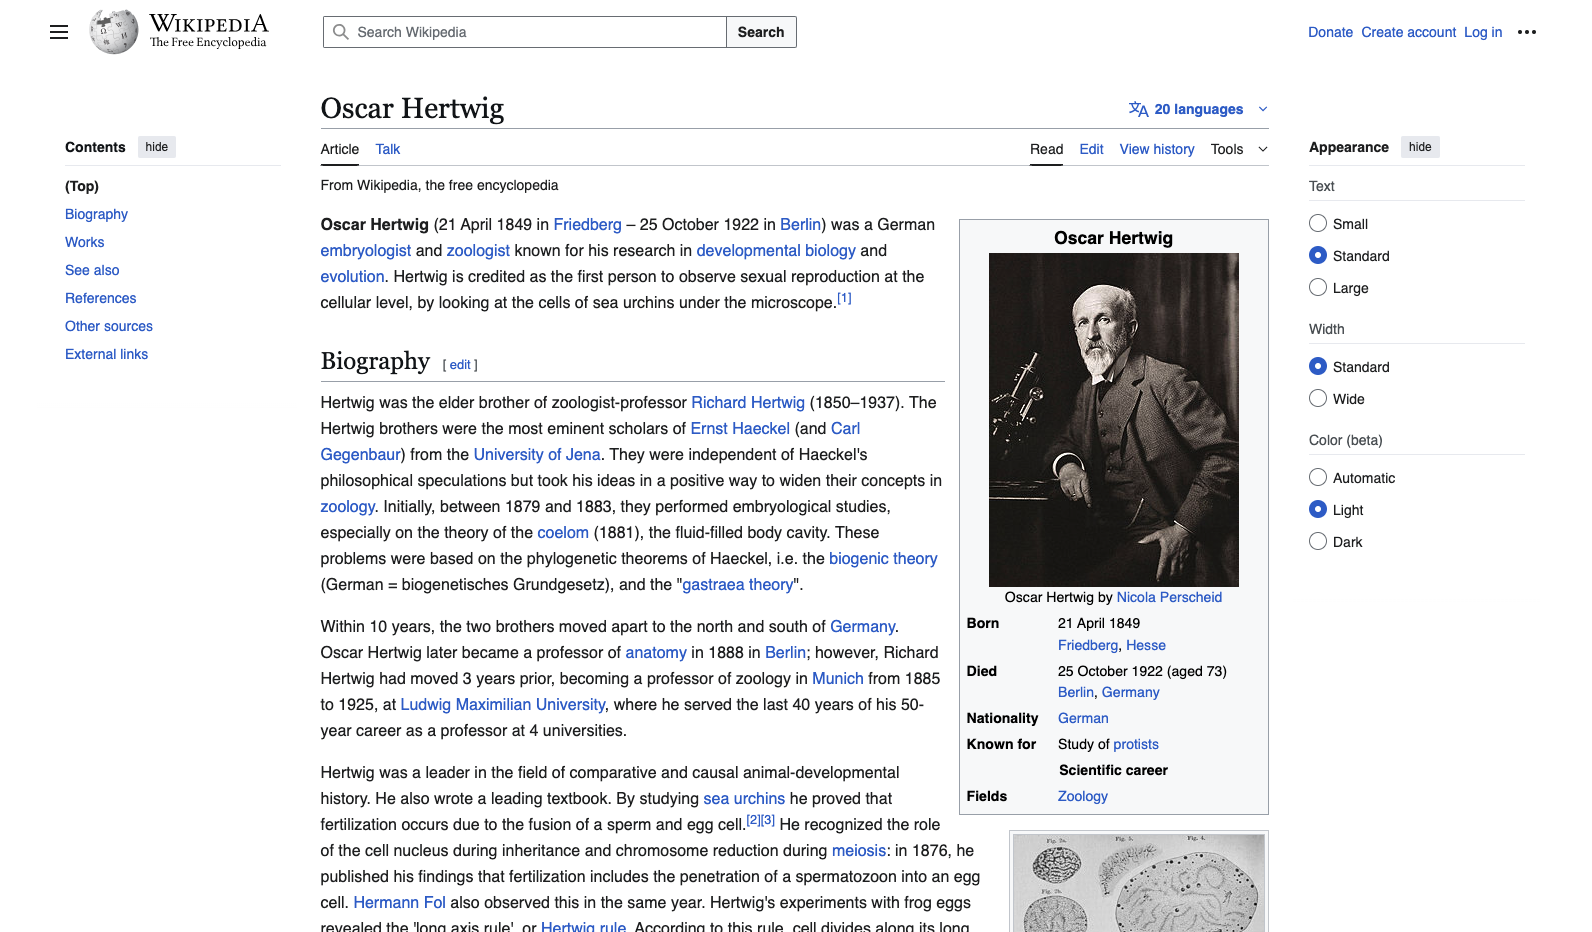
\includegraphics[width=\textwidth]{img/enwiki_example.png}
    \caption[English Wikipedia excerpt for the article Oscar Hertwig]{\textbf{English Wikipedia Excerpt for the Article Oscar Hertwig.} 
    The screenshot shows the English Wikipedia entry for Oscar Hertwig. It provides dense biographical and scientific information, mentioning concepts such as the coelom theory, biogenetic law, gastraea theory, the role of the nucleus, and chromosome reduction during meiosis. The article also lists detailed academic positions, institutions, and references to other scholars.
    The English Wikipedia version preserves domain-specific details and dense scientific terminology, which makes it comprehensive but potentially less accessible to non-expert readers. This serves as the baseline for comparison against the Simple English Wikipedia version.}
    \label{fig:enwiki_oscar}
\end{figure}
\clearpage
\begin{figure}[H]
    \centering
    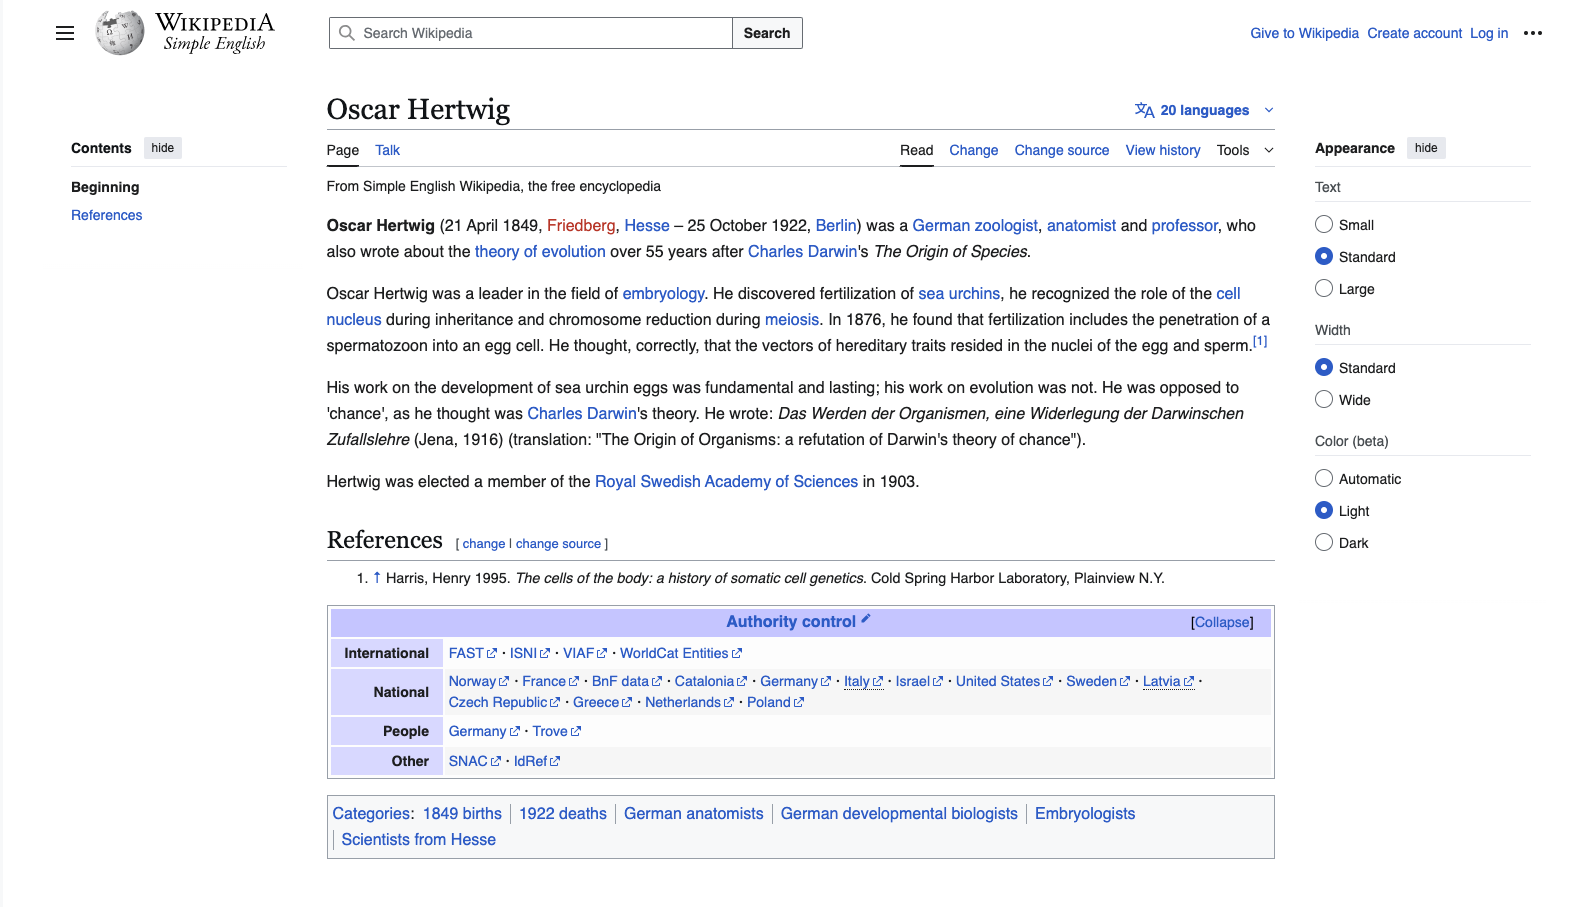
\includegraphics[width=\textwidth]{img/simplewiki_example.png}
    \caption[Simple English Wikipedia excerpt for the article Oscar Hertwig]{\textbf{Simple English Wikipedia Excerpt for the Article Oscar Hertwig.} 
    The screenshot shows the corresponding Simple English entry. While it preserves some key scientific terms such as fertilization of sea urchins, the role of the nucleus, and chromosome reduction during meiosis, it omits many details present in the English version (e.g., coelom theory, gastraea theory, specific academic posts, and references to other scientists).
    The Simple English version demonstrates common simplification strategies such as deletion, rephrasing, and structural reduction, showing how simplification improves readability but also leads to information loss, which is central to the research objective of this thesis.}
    \label{fig:simplewiki_oscar}
\end{figure}

\section{Data Source and Title matching}
The first step of data collection prepares the datasets needed to quantify information loss between English Wikipedia (EW) and Simple English Wikipedia (SEW). We extract EW and SEW articles from the \href{https://dumps.wikimedia.org/enwiki/}{\color{blue} Wikimedia dump service}.

\autoref{fig:DataCollectionPipeline} shows the overall data preparation pipeline. In the initial step, we parse the raw Wikipedia dumps to extract the text and metadata required for aligning articles and assigning topic labels for ORES prediction.

We use the \href{https://academictorrents.com/details/517bd4636dbb4b148374145e26c20f61ac63c093}{\color{blue} enwiki-20250301-pages-articles-multistream.xml.bz2}\cite{enwiki} and \href{https://mirror.clarkson.edu/wikimedia/simplewiki/20250301/}{\color{blue} simplewiki-20250301-pages-articles-multistream.xml.bz2} XML dumps published on March 1, 2025. We chose these dumps because they were the latest available at the time of preparing the thesis proposal.

For each article in the Simple English Wikipedia, we parse the XML data using Python’s \href{https://docs.python.domainunion.de/3/library/xml.etree.elementtree.html}{\color{blue} ElementTree} library. We extract the title and body text, remove MediaWiki-specific markup such as templates, file links, references, and formatting symbols, and then extract the first paragraph as the first block of meaningful text at least five words and not starting with markup.

We parse English Wikipedia in a similar way but add logic to extract category tags embedded in the article body. We then match the lowercase titles between SEW and EW, resulting in 261,768 aligned article pairs that form the basis for downstream comparisons.

In parallel, we parse the SQL dump \href{https://dumps.wikimedia.org/enwiki/}{\color{blue} enwiki-20250301-page.sql} to retrieve the mapping between article titles and their corresponding page ids. These IDs are used in the next stage to fetch the latest revision IDs through the MediaWiki API.

\begin{figure}[H]
    \centering
    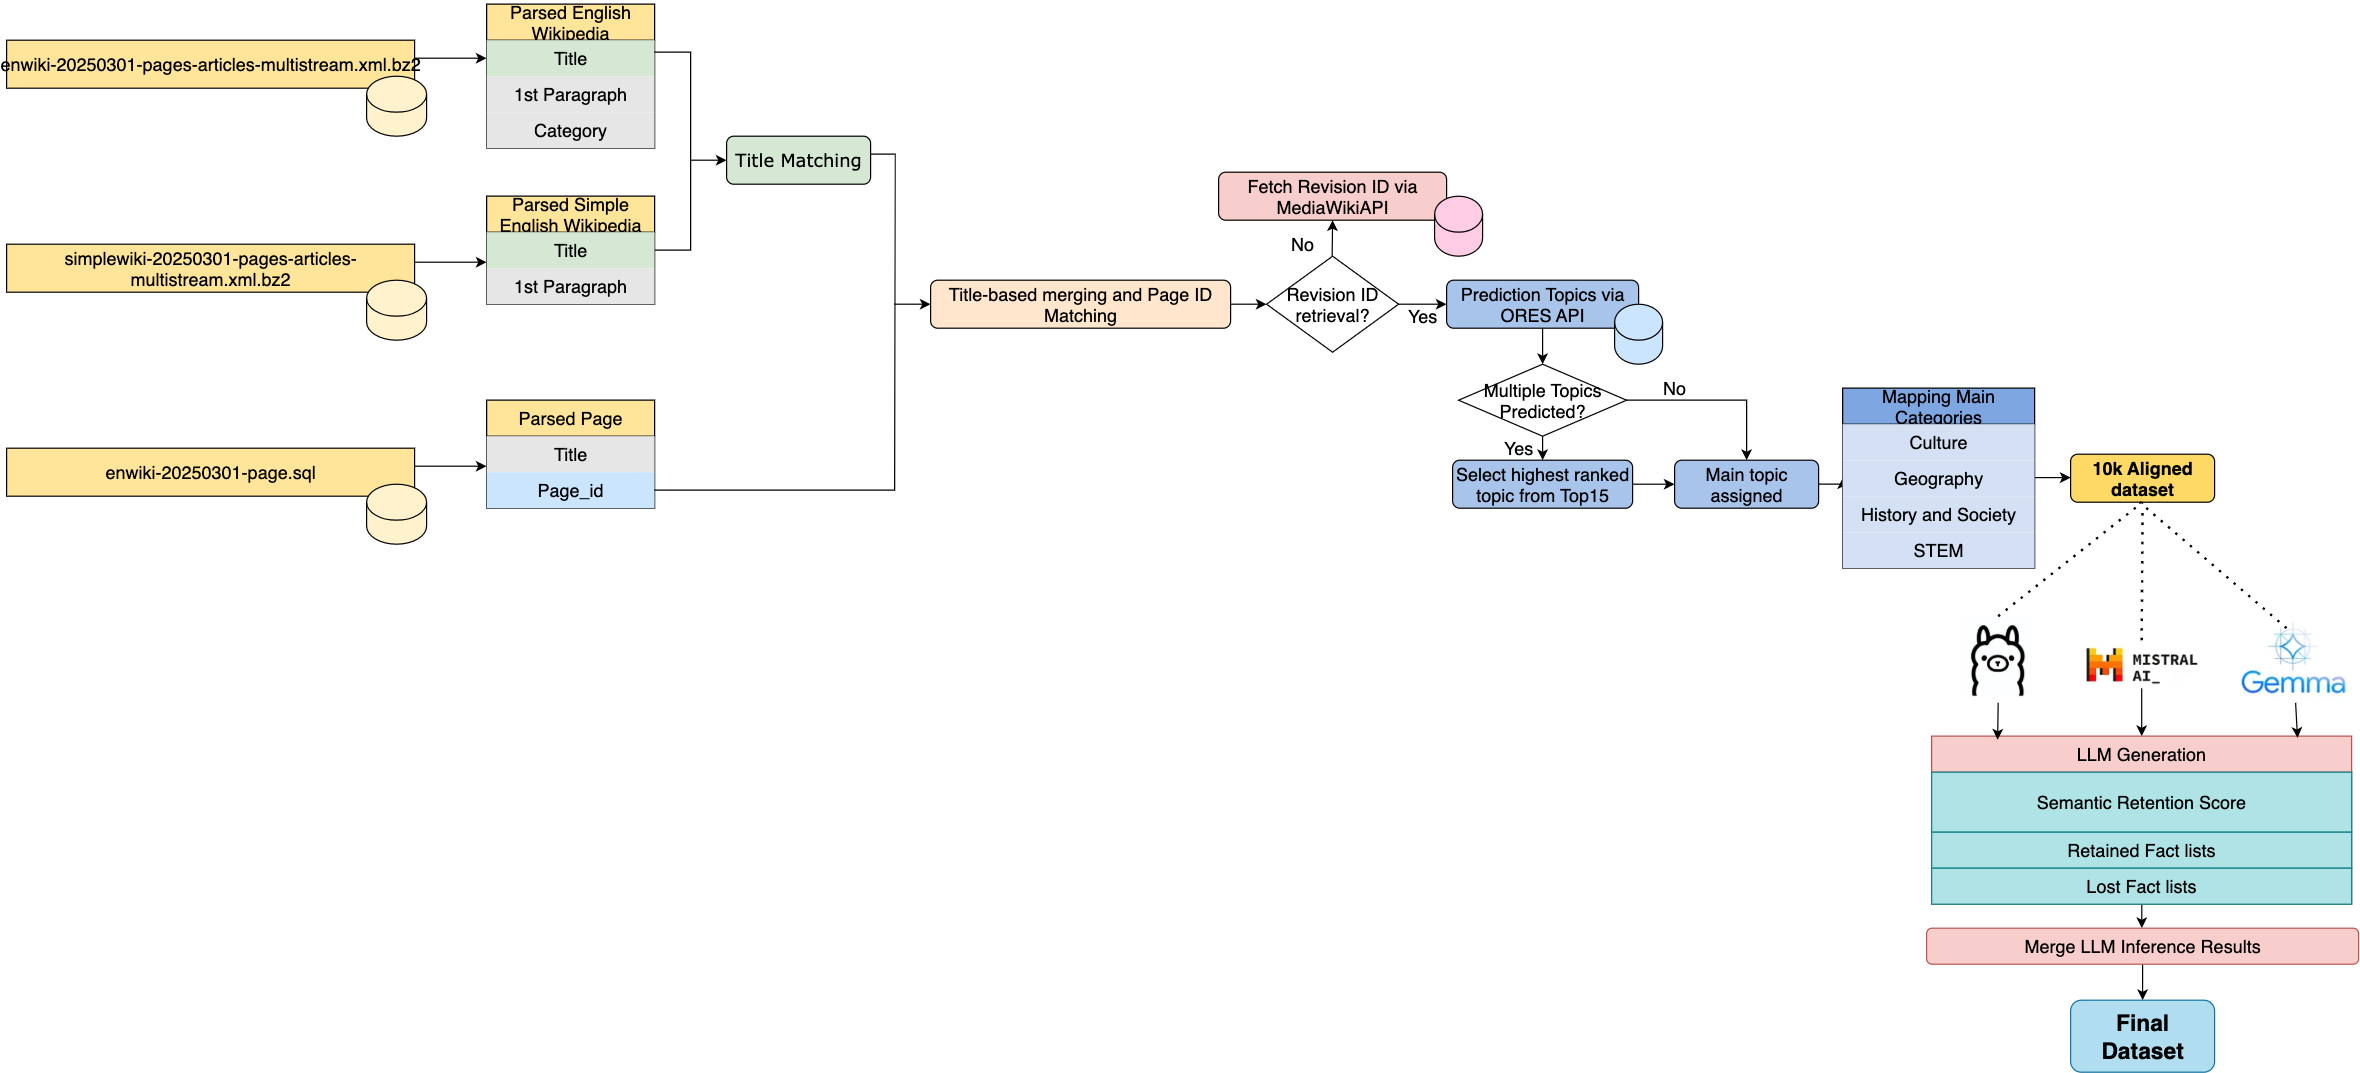
\includegraphics[width=\textwidth]{img/DataCollectionPipeline.png}
    \caption[Data Collection and Processing Pipeline]{\textbf{Data Collection and Processing Pipeline.} 
    The figure illustrates the end-to-end workflow for constructing the final dataset. Raw Wikipedia and Simple English Wikipedia dumps are parsed and preprocessed to extract titles, first paragraphs, and categories. Title-based matching ensures alignment between English and Simple English articles, followed by page ID retrieval and topic prediction using the ORES API. Articles are filtered to retain four main topic categories (Culture, Geography, History and Society, STEM). The aligned pairs are then processed with three Large Language Models (LLaMA, Mistral, and Gemma), which generate semantic retention scores and lists of retained and lost facts. These outputs are merged into the final dataset. 
    This pipeline ensures a systematic integration of raw Wikipedia resources with LLM-based evaluation, enabling large-scale analysis of information loss across topics.}
    \label{fig:DataCollectionPipeline}
\end{figure}

\section{Page ID and Revision ID Retrieval}

After extracting the raw text, we merge the SEW and EW datasets based on normalized article titles. 

To prepare for retrieving Revision ID in a further step, we attach the corresponding \texttt{page\_id} using the \href{https://dumps.wikimedia.org/enwiki/}{\color{blue} enwiki-20250301-page.sql} dump, which contains mappings between article titles and their associated page identifiers. 

During this merging step, the number of matched rows increases from 261{,}768 to 340{,}441. This increase results from a one-to-many mapping between article titles and page IDs. While Wikipedia enforces unique article titles for main articles, the SQL dump includes additional namespaces such as redirects, talk pages, or disambiguation pages. These entries often share the same title string but correspond to different \texttt{page\_id} values. Each such combination is retained as a separate row, leading to duplication in the merged dataset. 

To retrieve the most recent revision metadata for each article, we query the MediaWiki API using the associated \texttt{page\_id}. We run this as a parallelized process with retry mechanisms to efficiently collect revision IDs across more than 340,313 entries.

In total, we successfully retrieve 340,313 revision IDs, covering 99.96\% of the matched dataset. We use these values as input for the subsequent topic prediction step.

\section{ORES Topic Prediction and Main Topic Assignment}
\label{sec:ores_topic}
To support topic-level analysis for Research Question 2, we predict article-level topics using the \href{https://www.mediawiki.org/wiki/ORES}{\color{blue} ORES} model, a machine-learning system maintained by the Wikimedia Foundation. Each English Wikipedia (EW) article is first assigned a revision ID via the MediaWiki API. Using this revision ID, we query the \href{https://ores.wikimedia.org/docs}{\color{blue} ORES API}, which returns a list of predicted topics based on the article’s revision-level features. 

We analyze the full distribution of ORES-assigned topics across 340{,}313 unique article pairs with retrieved revision IDs. Because each article can have multiple topics, the distribution spans a large set of fine-grained categories.

To reduce complexity and enable stratified sampling, we extract the 15 most frequent topics from the full distribution (see Appendix, Figures \ref{fig:FullORESTopicDist} and \ref{fig:FullORESTop15Dist}). These top 15 topics cover the majority of articles and provide the basis for assigning a main topic to each article. We select the main topic as the most frequent label among those assigned to the article within the top 15. We exclude articles with no overlap.

Using this filtered set, we construct a sample of 10,000 article pairs. For each of the top 15 topics, we sample articles proportionally to their frequency. If the available articles for a topic fall short of the quota, we supplement the sample with articles from other topics in descending frequency until we reach 10,000.

Finally, we inspect the topic distribution in the sampled dataset (see Appendix, Figures \ref{fig:10kORESTopicDist} and \ref{fig:10kORESTop15Dist}). Each article retains its full ORES-assigned topic list, but we also assign one designated main topic from the top 15. This allows us to group the data consistently under four broader categories for downstream analysis.

\section{Mapping Main Categories}

To align with our research goal of topic-level information loss analysis, we restrict our dataset to articles whose main topic is among the top 15 most frequent topics predicted by ORES. These topics are further mapped into four broader knowledge categories \textbf{Culture, Geography, History and Society, and STEM} to enable high-level comparisons across different domains of knowledge. 

Table~\ref{tab:main_category_examples} illustrates how ORES topics map into the four categories by providing representative article titles. This clarifies the kinds of content that belong to each category.

\begin{table}[H]
\centering
\caption{Examples of article titles within each main category.}
\label{tab:main_category_examples}
\renewcommand{\arraystretch}{1.2}
\setlength{\tabcolsep}{12pt}
\begin{tabular}{l l}
\toprule
\textbf{Main Category} & \textbf{Example Article Titles} \\
\midrule
Culture & \textit{Holliday Grainger}, \textit{Jake Gyllenhaal} \\
Geography & \textit{Boundary Park}, \textit{Noguères} \\
History and Society & \textit{Tax Deduction}, \textit{2019–2020 peruvian constitutional crisis} \\
STEM & \textit{Enhanced Geothermal System}, \textit{Colorectal Surgery} \\
\bottomrule
\end{tabular}
\end{table}

We consolidate fine-grained ORES topics into interpretable knowledge areas through this mapping. For example, \texttt{Culture.Biography.Biography*} and \texttt{Culture.Sports} fall under \textbf{Culture}, while \texttt{Geography.Regions.Asia.Asia*} and \texttt{Geography.Regions.Europe.Europe*} fall under \textbf{Geography}. And, we group topics related to education, history, politics, and society under \textbf{History and Society} and \texttt{STEM.STEM*} is mapped directly to \textbf{STEM}. 

This rule-based mapping is guided by the hierarchical structure of the \href{https://www.mediawiki.org/wiki/ORES/Articletopic}{\color{blue} ORES Articletopic model} maintained by MediaWiki. The resulting column \texttt{main\_category} in the final dataset supports category-based analysis and comparison across knowledge domains. A full overview of the ORES topic taxonomy is provided in the Appendix (see Figure \ref{fig:ORESHierarchy}) to give context on how the fine-grained topics were grouped into broader categories. A complete overview of the 15 ORES topics and their corresponding main categories is provided in \autoref{tab:TopicToCategoryMap} in the Appendix.

\section{LLM Generation: LLaMA, Mistral, Gemma}

To generate semantic retention outputs for each aligned article pair, we run inference using three large language models: LLaMA-3-8B-Instruct\footnote{\url{https://ollama.com/library/llama3:8b}}, Mistral-7B-Instruct-v0.3\footnote{\url{https://ollama.com/library/mistral:7b-instruct-v0.3-q8_0}}, and Gemma-2-9B\footnote{\url{https://ollama.com/library/gemma2:9b}}. For simplicity, we hereafter refer to them as LLaMA, Mistral, and Gemma. We apply the same prompt template for all three models, as shown in \autoref{fig:PromptConfiguration} in the Methods chapter, with the full prompt templates provided in Appendix~\ref{appendix:prompts}.

Each input pair consists of the first paragraph from the English Wikipedia article and its corresponding Simple English Wikipedia version. The models are prompted to output a JSON-formatted response containing: a Semantic Retention Score (0--100\%), a list of retained facts, and a list of lost facts. 

We implement the generation process using \href{https://ollama.com/}{\color{blue}
Ollama} and we run inference on 10,000 sampled article pairs and track progress through log files to prevent reprocessing completed entries.

\section{Parsing and Merging LLM Outputs}

This section elaborates on the procedures used to extract and merge structured outputs from the raw responses generated by the LLMs. Although the prompts explicitly instructed models to return outputs in a JSON format containing a semantic retention score, retained facts, and lost facts, many responses were embedded in free-form text or markdown-wrapped code blocks, often containing escape characters or formatting inconsistencies. Therefore, model-specific parsers were developed to extract relevant information. 

\paragraph{Model-Specific Parsing.}
Each LLM produced outputs with different formatting behaviors. LLaMA often returned markdown code blocks (e.g., \verb|json ... |) or partial JSON structures mixed with explanatory text. To handle this, we designed the LLaMA parser as a multi-stage process: it first attempted to extract structured JSON and then applied fallback heuristics with regular expressions to recover retention scores and fact lists.

Mistral frequently produced multiple JSON-like blocks or fragmented lists. We addressed this by parsing all valid JSON blocks in reverse order and then applying fallback methods for list reconstruction and custom cleaning to remove formatting noise.

Gemma, formatted through the Ollama API, typically wrapped its responses in a \verb|response='...'| string with nested escape sequences. We built the parser to first unescape and normalize the response string and then extract the JSON content enclosed in \verb|json ... | blocks.

\paragraph{Preprocessing and Cleaning.}
Common cleaning steps across all parsers removed newline escape sequences, HTML entities, trailing commas, and Unicode escape codes. We implemented a shared utility function, \verb|cleanup_json()|, to normalize string inputs before applying \verb|json.loads()| or regular expression matching.

\paragraph{Merging Parsed Outputs.}
After parsing, we stored the outputs for each model in separate dataframes and merged them into the final master dataset using article titles as the join key. For LLaMA, we overwrote problematic initial generations with rerun results. Before merging, we removed duplicate entries to ensure a one-to-one mapping.

The final merged dataset includes semantic retention scores, retained fact lists, and lost fact lists for each aligned article pair across all three models. We then computed descriptive statistics to identify missing or invalid outputs. Table \ref{tab:llm-parsing-summary} summarizes the parsing success rates and outlier proportions per model. 

\section{Final Dataset Construction}

After parsing and aligning the outputs from all three LLMs, we finalize the dataset by combining essential columns into a final dataset file. Specifically, we retain the following attributes: article title, first paragraphs from English Wikipedia and Simple English Wikipedia, predicted ORES topics and main topic, mapped main category, page and revision identifiers, and the semantic retention scores and retained/lost fact lists generated by LLaMA, Mistral, and Gemma.

We verify the integrity of these attributes to ensure the dataset is well-structured for downstream analysis. All entries are preserved in the final dataset, providing a comprehensive view of semantic retention across models and topics. The finalized dataset, saved as \verb|final_dataset.csv|, contains 10,000 article pairs and serves as the core evaluation resource for this thesis. 

\autoref{fig:10kFinalCategoryDist} shows the distribution of articles across the four main categories (Culture, Geography, STEM, and History and Society).

\begin{table}[h]
\centering
\begin{tabular}{lcccc}
\toprule
\textbf{Model} & \textbf{Total Samples} & \textbf{Missing Values} & \textbf{Outliers (\textgreater100)} & \textbf{Invalid Rate (\%)} \\
\midrule
LLaMA & 10,000 & 202 & 2 & 2.04 \\
Mistral & 10,000 & 31 & 1 & 0.32 \\
Gemma & 10,000 & 127 & 0 & 1.27 \\
\bottomrule
\end{tabular}
\caption{Parsing summary per model, including number of missing scores and outliers.}
\label{tab:llm-parsing-summary}
\end{table}

\begin{figure}[H]
    \centering
    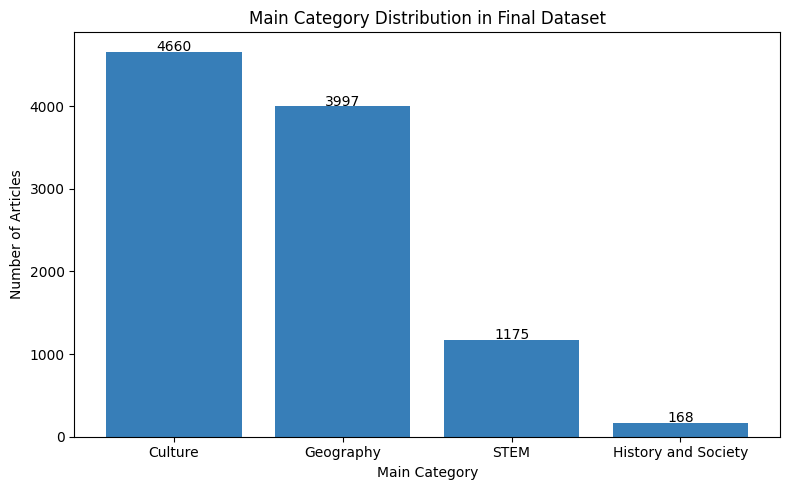
\includegraphics[width=\textwidth]{img/10kFinalCategoryDist.png}
    \caption[Main category distribution in the 10k final dataset]{\textbf{Main Category Distribution in the 10k Final Dataset.} 
    The bar chart shows the number of articles assigned to each of the four main categories in the 10k final dataset. Culture (4,660 articles) and Geography (3,997 articles) account for the majority of entries, while STEM (1,175 articles) and History and Society (168 articles) are represented to a smaller extent. Each article is assigned a single main category. 
    This distribution reflects the natural prevalence of Culture and Geography topics in Wikipedia.}
    \label{fig:10kFinalCategoryDist}
\end{figure}


\section{Human Validation Subset}
\label{sec:human_subset}
To assess the reliability of LLM-generated semantic retention scores, we construct a manually verified subset of 50 article pairs sampled from the finalized dataset. We balance this subset across the four main categories: Culture, Geography, STEM, and History and Society.

We follow two constraints during sampling:
(1) we prioritize article pairs that we had already manually validated before the midterm presentation to retain those results, and
(2) we ensure proportional representation of the four main categories.

We first include all articles from a predefined list of 9 manually annotated titles. We then perform stratified sampling from the remaining pool to fill the quota, assigning about 12–13 samples to each main category (see Figure \ref{fig:HumanValidationCategoryDist}).

\begin{figure}[H]
    \centering
    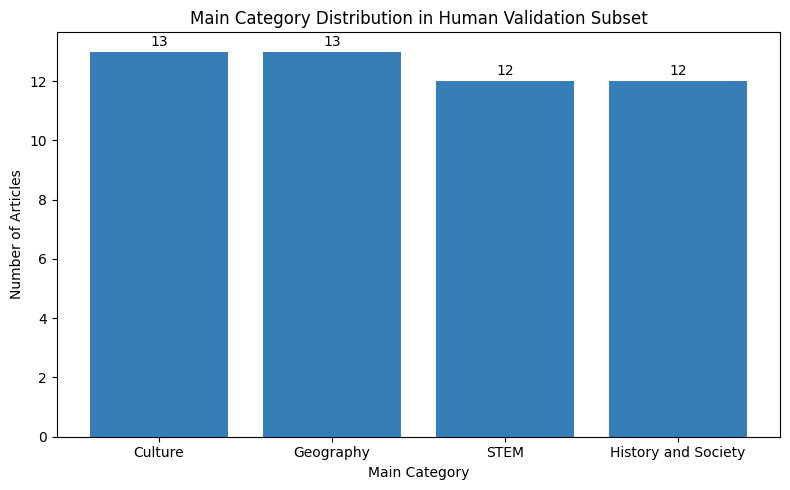
\includegraphics[width=\textwidth]{img/HumanValidationCategoryDist.png}
    \caption[Main category distribution in the Human Validation subset]{\textbf{Main Category Distribution in the Human Validation Subset.} 
    The bar chart shows the distribution of main categories for the 50 articles selected for human validation. The subset contains 13 articles from Culture, 13 from Geography, 12 from STEM, and 12 from History and Society. 
    The nearly balanced representation across the four categories ensures that human evaluation covers all main topics of the thesis, allowing assessment of whether simplification and information loss show consistent patterns across domains with different characteristics.}
    \label{fig:HumanValidationCategoryDist}
\end{figure}

\chapter{Methodology}
This chapter presents the methodological framework used to quantify information loss between English Wikipedia and Simple English Wikipedia. We begin by defining the concepts of information loss and semantic retention. We then introduce the LLM-based automatic evaluation framework, which includes prompt design and model selection, the generation of semantic retention scores on a 0–100\% scale, the extraction of retained and lost fact lists, and an internal consistency check that links model-assigned scores to fact counts. Finally, we describe the human validation process, outlining the annotation scope and guidelines, the evaluation procedure and metrics (accuracy, precision, recall, and F1), and the analysis of inter-annotator agreement to assess consistency among human judgments.

\section{Definition of Information Loss and Semantic Retention}

Information loss is a phenomenon in the text simplification process, as removing linguistic complexity often comes at the cost of omitting important details from the original text\cite{trienes2024infolossqacharacterizingrecoveringinformation}. 

Building on this definition, in this thesis, we define information loss as any facts that are present in the English Wikipedia (EW) article but missing in the corresponding Simple English Wikipedia (SEW) version. Specifically, we restrict the scope of information loss to facts that are originally present in the EW article. If a fact derived from the original article does not appear in the simplified version, we consider that an instance of information loss. Conversely, we do not evaluate facts that appear only in the simplified version, as they lie outside the defined scope of comparison. 

We also introduce the complementary concept of semantic retention. Semantic retention refers to the proportion of original information that remains intact in the simplified version. Rather than quantifying information loss directly, we ask large language models (LLMs) to generate semantic retention scores ranging from 0 to 100. These scores reflect how much of the original semantic content is retained in the simplified text: a higher score implies better information preservation, while a lower score indicates greater information loss. 

Thus, in this study, information loss and semantic retention are inherently linked:
\[
\text{Information Loss} = 100 - \text{Semantic Retention Score}
\]

\section{LLM-Based Automatic Evaluation Framework}

This section elaborates on the automatic evaluation framework used to quantify information loss by leveraging large language models (LLMs). The framework enables the systematic assessment of how much semantic content is preserved between English Wikipedia articles and their Simple English Wikipedia counterparts. 

The framework consists of four components:  
(1) the design of a consistent prompt and the selection of LLMs (\autoref{subsec:prompt}), 
(2) the generation of semantic retention scores for aligned article pairs (\autoref{subsec:score}),  
(3) the extraction of retained and lost fact lists generated by LLMs (\autoref{subsec:factlists}), and
(4) the postprocessing procedures to ensure reliable parsing of structured responses (\autoref{subsec:consistency}).  

\subsection{Prompt Design and Model Selection}
\label{subsec:prompt}
To ensure consistent outputs, we design a structured prompt configuration that instructs the LLM to analyze two aligned paragraphs and perform three tasks:  
(1) identify and list the key information that is retained in the simplified paragraph,  
(2) identify and list the information that is lost, and  
(3) calculate the overall semantic retention score as a percentage.  

An overview of the prompt logic is shown in \autoref{fig:PromptConfiguration}. Also, the exact prompt template used in our experiments is provided in \autoref{appendix:prompts}. And, the prompt is designed to make expectations explicit: it defines the input context, describes the required output format, and provides detailed instructions so that the model produces responses in a structured JSON schema.

\begin{figure}[H]
    \centering
    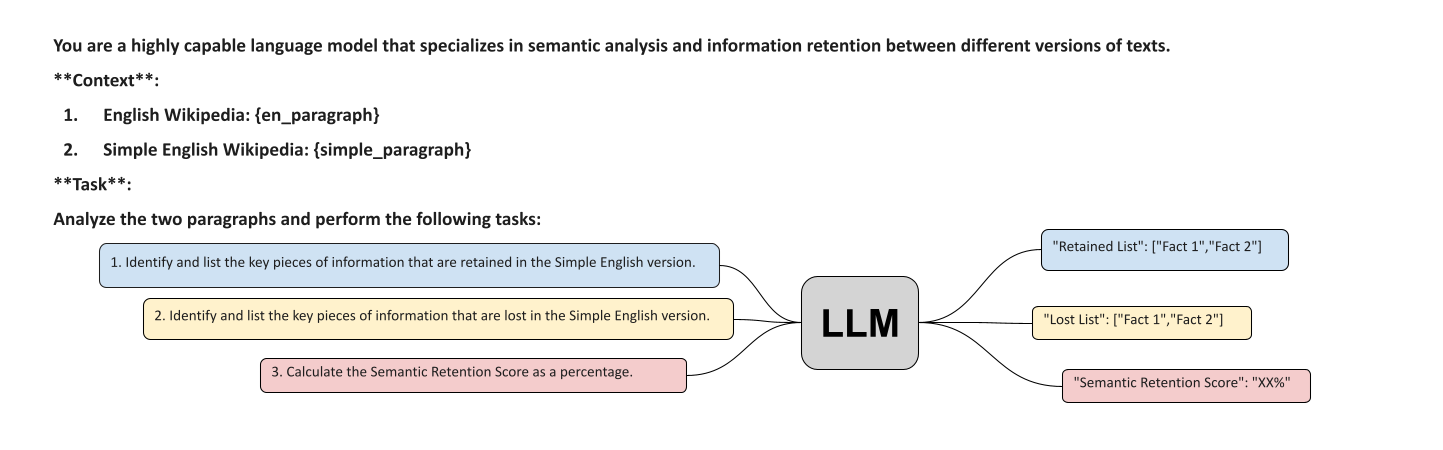
\includegraphics[width=\textwidth]{img/PromptConfiguration.png}
    \caption[Prompt design for LLM-based evaluation of semantic retention]{\textbf{Prompt Design for LLM-Based Evaluation of Semantic Retention.} 
    The figure illustrates the structured prompt configuration used to guide the LLM in analyzing information retention. In this setup, the model receives two aligned paragraphs. One from English Wikipedia and one from Simple English Wikipedia and is instructed to (1) identify retained facts, (2) identify lost facts, and (3) calculate a semantic retention score as a percentage. The model outputs results in a structured JSON format with three fields: a retained list, a lost list, and the retention score. 
    This design ensures that the LLM produces interpretable and standardized outputs, which are critical for reliable parsing, quantitative evaluation, and subsequent downstream analysis.}
    \label{fig:PromptConfiguration}
\end{figure}

We experiment with the pre-designed prompt using three models: LLaMA-3-8B-Instruct\footnote{\url{https://ollama.com/library/llama3:8b}}, Mistral-7B-Instruct-v0.3\footnote{\url{https://ollama.com/library/mistral:7b-instruct-v0.3-q8_0}}, and Gemma-2-9B\footnote{\url{https://ollama.com/library/gemma2:9b}}.  

\subsection{Semantic Retention Score Generation}
\label{subsec:score}
For each aligned article pair, the LLM is instructed to calculate a \textit{Semantic Retention Score}, representing the percentage of original semantic content that is preserved in the simplified version. The score ranges from 0 to 100, where a higher score indicates greater preservation of factual information and a lower score corresponds to higher information loss.  

The score is generated by the LLM through its own semantic comparison of the two paragraphs. This approach makes it possible to evaluate 10,000 article pairs at scale without manual effort. The numeric value is then extracted from the model’s response using a parsing pipeline that standardizes variations in output formatting.  

Within this thesis, the semantic retention score serves as the primary quantitative indicator of simplification quality.  

\subsection{Retained and Lost Fact List Extraction}
\label{subsec:factlists}
In addition to the scalar retention score, the prompt instructs the LLM to produce two lists derived from the English Wikipedia paragraph: 
the \textit{Retained List}, which contains facts that are also present in the Simple English versionn and 
the \textit{Lost List}, which contains facts that are missing in the Simple English version. 

This ensures that both retained and lost facts are defined relative to the original English Wikipedia paragraph, focusing the evaluation on how much of the source information is preserved during simplification.  

\subsection{Internal Consistency Check}
\label{subsec:consistency}
To evaluate whether each LLM applies a consistent internal logic when estimating semantic retention, we compare the retention score generated by the model with an expected score that can be calculated directly from its own fact lists. The idea is that if the model first identifies which facts are retained and which are lost, then the percentage of retained facts relative to the total (retained + lost) should approximately align with the overall score it reports.  

Formally, the expected score is defined as:  

\[
\text{Expected Score (\%)} = \frac{\# \text{Retained Facts}}{\# \text{Retained Facts} + \# \text{Lost Facts}} \times 100
\]
Here, the symbol $\#$ denotes the number of facts in each category.

This consistency check helps us determine whether the model’s numeric judgment of semantic retention score is in line with its own fact-level analysis. Large differences between the two would suggest that the model gives a score that does not match the facts it has listed, indicating a lack of internal consistency in its evaluation process.

\section{Human Validation}
\label{sec:human_validation}
This section describes the human validation setup that complements the automatic LLM-based evaluation. It covers three components: 
(1) the annotation scope and guidelines followed by human annotators (\autoref{subsec:annotation}), 
(2) the validation procedure and the metrics used to compare LLM outputs with human-annotated ground truth (\autoref{subsec:validation}), and 
(3) inter-annotator agreement analysis to assess the consistency of human annotations (\autoref{subsec:iaa}).  
\subsection{Annotation Scope and Guideline}
\label{subsec:annotation}
To assess the quality and reliability of the LLM-generated semantic retention scores and fact lists, we construct a human validation subset of 50 article pairs (see \autoref{sec:human_subset}). Annotators receive the original English Wikipedia paragraph along with the Simple English Wikipedia paragraph, and manually extract all key facts present in the original version. Each fact is labeled as either \textit{Retained} if it appears in the simplified text, or \textit{Lost} if it is omitted.  

Annotators follow a consistent set of guidelines to decide which facts to extract. They include only concrete information such as names, dates, events, and numbers from English Wikipedia. Using these rules, each annotator creates two lists: one with facts that appear in the Simple English wikipedia (\textit{Retained}) and one with facts that do not (\textit{Lost}). These human-annotated lists serve as the ground truth for comparing the quality of the LLM outputs.  

\subsection{Validation Procedure and Metrics}
\label{subsec:validation}

We evaluate the quality of the LLM-generated retained and lost fact lists by comparing them against the human-annotated ground truth for each article pair. For each model, we compute precision, recall, accuracy, and F\(1\)-score based on the alignment between model outputs and human annotations.

To make this comparison, we treat retained facts as the positive class (P) and lost facts as the negative class (N). Thus, a fact is considered positive if it appears in the Simple English Wikipedia paragraph (i.e., retained) and negative if it is omitted during simplification (i.e., lost).

The classification proceeds as follows. A fact is counted as a \textit{true positive (TP)} when both the human annotator and the LLM mark it as retained. It becomes a \textit{false positive (FP)} if the LLM marks a fact as retained but the human annotator does not. Conversely, a \textit{false negative (FN)} occurs when the human annotator considers a fact retained but the model fails to include it. Finally, if both sides consistently classify a fact as lost, or if the fact is omitted entirely, it is treated as a \textit{true negative (TN)}.

The special case of \textit{not listed} occurs when a human annotator identifies a fact in the original English Wikipedia paragraph, but the LLM does not include it in either the retained or lost list. Because human annotators extract facts at a more fine-grained level, LLM outputs often omit such details. In this case, the evaluation depends on the human judgment: If the human marked the fact as retained, the omission is counted as a false negative. But, if the human marked it as lost, it is counted as a true negative. Table~\ref{tab:fact-classification} summarizes these classification rules.

\begin{table}[h]
\centering
\begin{tabular}{lll}
\toprule
\textbf{Human Judgement} & \textbf{LLM Class} & \textbf{Final Class} \\
\midrule
Retained & Retained & TP (True Positive) \\
Retained & Lost & FN (False Negative) \\
Lost & Retained & FP (False Positive) \\
Lost & Lost & TN (True Negative) \\
Lost & Not listed & TN (True Negative) \\
Retained & Not listed & FN (False Negative) \\
\bottomrule
\end{tabular}
\caption{Classification of facts based on comparison between human annotation and LLM output.}
\label{tab:fact-classification}
\end{table}

Based on these classifications, we compute the standard evaluation metrics as follows:  

\[
\text{Precision} = \frac{TP}{TP + FP}, \quad
\text{Recall} = \frac{TP}{TP + FN},
\]

\[
\text{Accuracy} = \frac{TP + TN}{TP + FP + TN + FN}, \quad
F_1 = \frac{2 \times \text{Precision} \times \text{Recall}}{\text{Precision} + \text{Recall}}
\]

\subsubsection*{Running Example (End-to-End): Oscar Hertwig}

As a single illustrative example, we use the case of \textit{Oscar Hertwig} to demonstrate the full workflow. The process is shown step by step based on the outputs generated by the LLaMA model.

\paragraph{Inputs.}
\textbf{English Wikipedia (EW):}\\
\textit{“Oscar Hertwig (21 April 1849 in Friedberg - 25 October 1922 in Berlin) was a German embryologist and zoologist known for his research in developmental biology and evolution. Hertwig is credited as the first person to observe sexual reproduction at the cellular level, by looking at the cells of sea urchins under the microscope.”}

\noindent
\textbf{Simple English Wikipedia (SEW):}\\
\textit{“Oscar Hertwig (21 April 1849), German zoologist, anatomist and professor, who also wrote about the theory of evolution over 55 years after Charles Darwin's ‘The Origin of Species’.”}

\paragraph{Step 1: LLM Generation.}\\

Given the EW-SEW pair, the LLaMA model outputs a \textbf{semantic retention score} of \textbf{67}.

\begin{table}[H]
\centering
\caption{Step 1: LLM-generated retained and lost facts (LLaMA).}
\label{tab:llm_lists_hertwig}
\renewcommand{\arraystretch}{1.2}
\setlength{\tabcolsep}{6pt}
\begin{tabularx}{\textwidth}{lX}
\toprule
\textbf{Type} & \textbf{Facts (as generated by LLM)} \\
\midrule
Retained (LLM) &
Oscar Hertwig was born on 21 April 1849; He was a German zoologist, anatomist, and professor; He wrote about the theory of evolution. \\
Lost (LLM) &
Hertwig observed sexual reproduction at the cellular level by looking at sea urchin cells under the microscope; Specific details about his research in developmental biology and evolution are missing. \\
\bottomrule
\end{tabularx}
\end{table}

\paragraph{Step 2: Internal Consistency Check.}\\

From the model’s own lists, the expected score is
\[
\text{Expected Score}=\frac{3}{3+2}\times100=60.
\]

\paragraph{Step 3: Human Annotation (Ground Truth).}\\

Annotators extract fine-grained facts from EW and label whether each is present in SEW.

\begin{table}[H]
\centering
\caption{Step 3  Human-annotated facts and labels.}
\label{tab:human_list_hertwig}
\renewcommand{\arraystretch}{1.15}
\setlength{\tabcolsep}{6pt}
\begin{tabularx}{\textwidth}{X c}
\toprule
\textbf{Fact (Human)} & \textbf{Label} \\
\midrule
Oscar Hertwig was born on 21 April 1849. & retained \\
He was born in Friedberg. & lost \\
He died on 25 October 1922. & lost \\
He died in Berlin. & lost \\
He was a German embryologist. & lost \\
He was a German zoologist. & retained \\
He was known for his research in developmental biology. & lost \\
He was also known for his research in evolution. & lost \\
Oscar Hertwig was the first person to observe sexual reproduction at the cellular level. & lost \\
Oscar Hertwig observed sexual reproduction by looking at the cells of sea urchins. & lost \\
Oscar Hertwig used a microscope to observe sea urchin cells. & lost \\
\bottomrule
\end{tabularx}
\end{table}

\paragraph{Step 4: Comparison and Fact-Level Validation.}\\

Each human fact is aligned with the LLM lists to assign TP/TN/FP/FN.

\begin{table}[H]
\centering
\caption{Step 4  LLaMA vs.\ Human fact comparison.}
\label{tab:llm_vs_human_hertwig}
\renewcommand{\arraystretch}{1.15}
\setlength{\tabcolsep}{6pt}
\begin{tabularx}{\textwidth}{X c c c c}
\toprule
\textbf{Facts by Human} & \textbf{Human List} & \textbf{LLaMA's List} & \textbf{Validation Status} & \textbf{Validation} \\
\midrule
Oscar Hertwig was born on 21 April 1849. & retained & retained & True & TP (True Positive) \\
He was born in Friedberg. & lost & Not listed & True & TN (True Negative) \\
He died on 25 October 1922. & lost & Not listed & True & TN (True Negative) \\
He died in Berlin. & lost & Not listed & True & TN (True Negative) \\
He was a German embryologist. & lost & Not listed & True & TN (True Negative) \\
He was a German zoologist. & retained & retained & True & TP (True Positive) \\
He was known for his research in developmental biology. & lost & lost & True & TN (True Negative) \\
He was also known for his research in evolution. & lost & lost & True & TN (True Negative) \\
Oscar Hertwig was the first person to observe sexual reproduction at the cellular level. & lost & lost & True & TN (True Negative) \\
Oscar Hertwig observed sexual reproduction by looking at the cells of sea urchins. & lost & lost & True & TN (True Negative) \\
Oscar Hertwig used a microscope to observe sea urchin cells. & lost & lost & True & TN (True Negative) \\
\bottomrule
\end{tabularx}
\end{table}

\paragraph{Step 5: Metric Computation.}\\

Using the counts from \autoref{tab:llm_vs_human_hertwig} (e.g., TP=2, TN=9, FP=0, FN=0):
\[
\text{Precision}=\frac{TP}{TP+FP}=1.00,\quad
\text{Recall}=\frac{TP}{TP+FN}=1.00,\quad\]
\[
\text{Accuracy}=\frac{TP+TN}{TP+FP+TN+FN}=1.00,\quad
F_1=\frac{2PR}{P+R}=1.00.
\]

\subsection{Inter-Annotator Agreement}
\label{subsec:iaa}
In addition to evaluating the reliability of LLM predictions against human annotations, we also assess the consistency of the human annotations themselves. For this purpose, we compute inter-annotator agreement (IAA) using Fleiss' $\kappa$ \cite{fleiss1971measuring},  which measures agreement among multiple annotators beyond chance. The statistic is defined as follows:

\[
\kappa = \frac{\bar{P} - \bar{P_e}}{1 - \bar{P_e}}
\]
where $\bar{P}$ denotes the observed agreement across annotators, and $\bar{P_e}$ is the expected agreement based on the marginal label distribution. Values of $\kappa$ range from $-1$ (complete disagreement) to $1$ (perfect agreement), with $0$ indicating agreement equivalent to chance. 
Following Landis and Koch (1977), values above 0.80 are interpreted as \textit{almost perfect agreement}\cite{landis1977measurement}. 
In this thesis, Fleiss’ $\kappa$ is applied to a subset of annotated articles to quantify the consistency among annotators, thereby providing a reliability benchmark for the fact-level human validation process.

\chapter{Results and Analysis}
This chapter presents empirical findings from the 10,000 Wikipedia–Simple English Wikipedia pairs and the 50-sample human validation set. We begin by providing an overview of the evaluation framework and model inference process. We then address the first research question by analyzing score distributions, conducting internal consistency checks, and comparing model with human judgments. After that, we present qualitative case studies to illustrate examples of high agreement and low agreement between models and human annotations. The second research question is examined through topic-wise analyses, focusing on retention patterns and validation metrics such as accuracy and F1. Finally, we summarize the key findings, highlighting the main insights gained from the analysis.

\section{Overview of the Framework and LLM Inference}
To evaluate information loss between English Wikipedia and Simple English Wikipedia, we employ three large language models (LLMs): LLaMA, Mistral, and Gemma. Each model is prompted to generate a semantic retention score ranging from 0 to 100 as well as lists of retained and lost facts for 10,000 aligned article pairs. The validity of generated scores is first checked to ensure values fall within the expected range.

\autoref{tab:validity_summary} presents the validity statistics of the generated semantic retention scores. Overall, the majority of values fall within the expected range (0-100), indicating that all three models are generally robust. Among them, Gemma demonstrates the highest stability, with no out-of-range values and 127 missing cases. Mistral generates the most consistently valid outputs, yielding only 32 invalid cases in total. By contrast, LLaMA generates more invalid outputs, with 202 missing scores and 2 values falling outside the valid range.

\begin{table}[H]
\centering
\caption{Validity summary of LLM-generated semantic retention scores (N=10,000 per model).}
\label{tab:validity_summary}
\begin{tabular}{lcccc}
\toprule
Model & N total & N valid (0-100) & N NA & N out-of-range \\
\midrule
LLaMA   & 10,000 & 9,796 & 202 & 2 \\
Mistral & 10,000 & 9,968 & 31  & 1 \\
Gemma   & 10,000 & 9,873 & 127 & 0 \\
\bottomrule
\end{tabular}
\end{table}

\section{Research Goal 1: Can LLMs Reliably Assess Information Loss?}
\subsection{Semantic Retention Score Distribution (10k Dataset)}
\autoref{tab:mean_median} summarizes the overall mean and median semantic retention scores based on valid outputs. Gemma generates the highest averages (mean 75.1, median 80.0), followed by Mistral (mean 66.65, median 75.0) and LLaMA (mean 65.62, median 67.0). This indicates that Gemma generally generates higher semantic retention scores across the dataset, while LLaMA and Mistral generate at a similar but lower level.

\begin{table}[H]
\centering
\caption{Overall mean and median semantic retention scores.}
\label{tab:mean_median}
\begin{tabular}{lccc}
\toprule
Model & Mean & Median & N valid \\
\midrule
LLaMA   & 65.62 & 67.0 & 9,796 \\
Mistral & 66.65 & 75.0 & 9,968 \\
Gemma   & 75.10 & 80.0 & 9,873 \\
\bottomrule
\end{tabular}
\end{table}

\autoref{fig:AvgScoresBoxplots} provides the distribution of scores across models. While Gemma clearly shifts toward higher values, LLaMA shows a more compact interquartile range, suggesting relatively consistent outputs around its mean. Mistral, in contrast, exhibits a broader spread, indicating greater variability in the scores it produces. These distributional patterns complement the summary statistics and highlight differences in output consistency across models.

\begin{figure}[H]
    \centering
    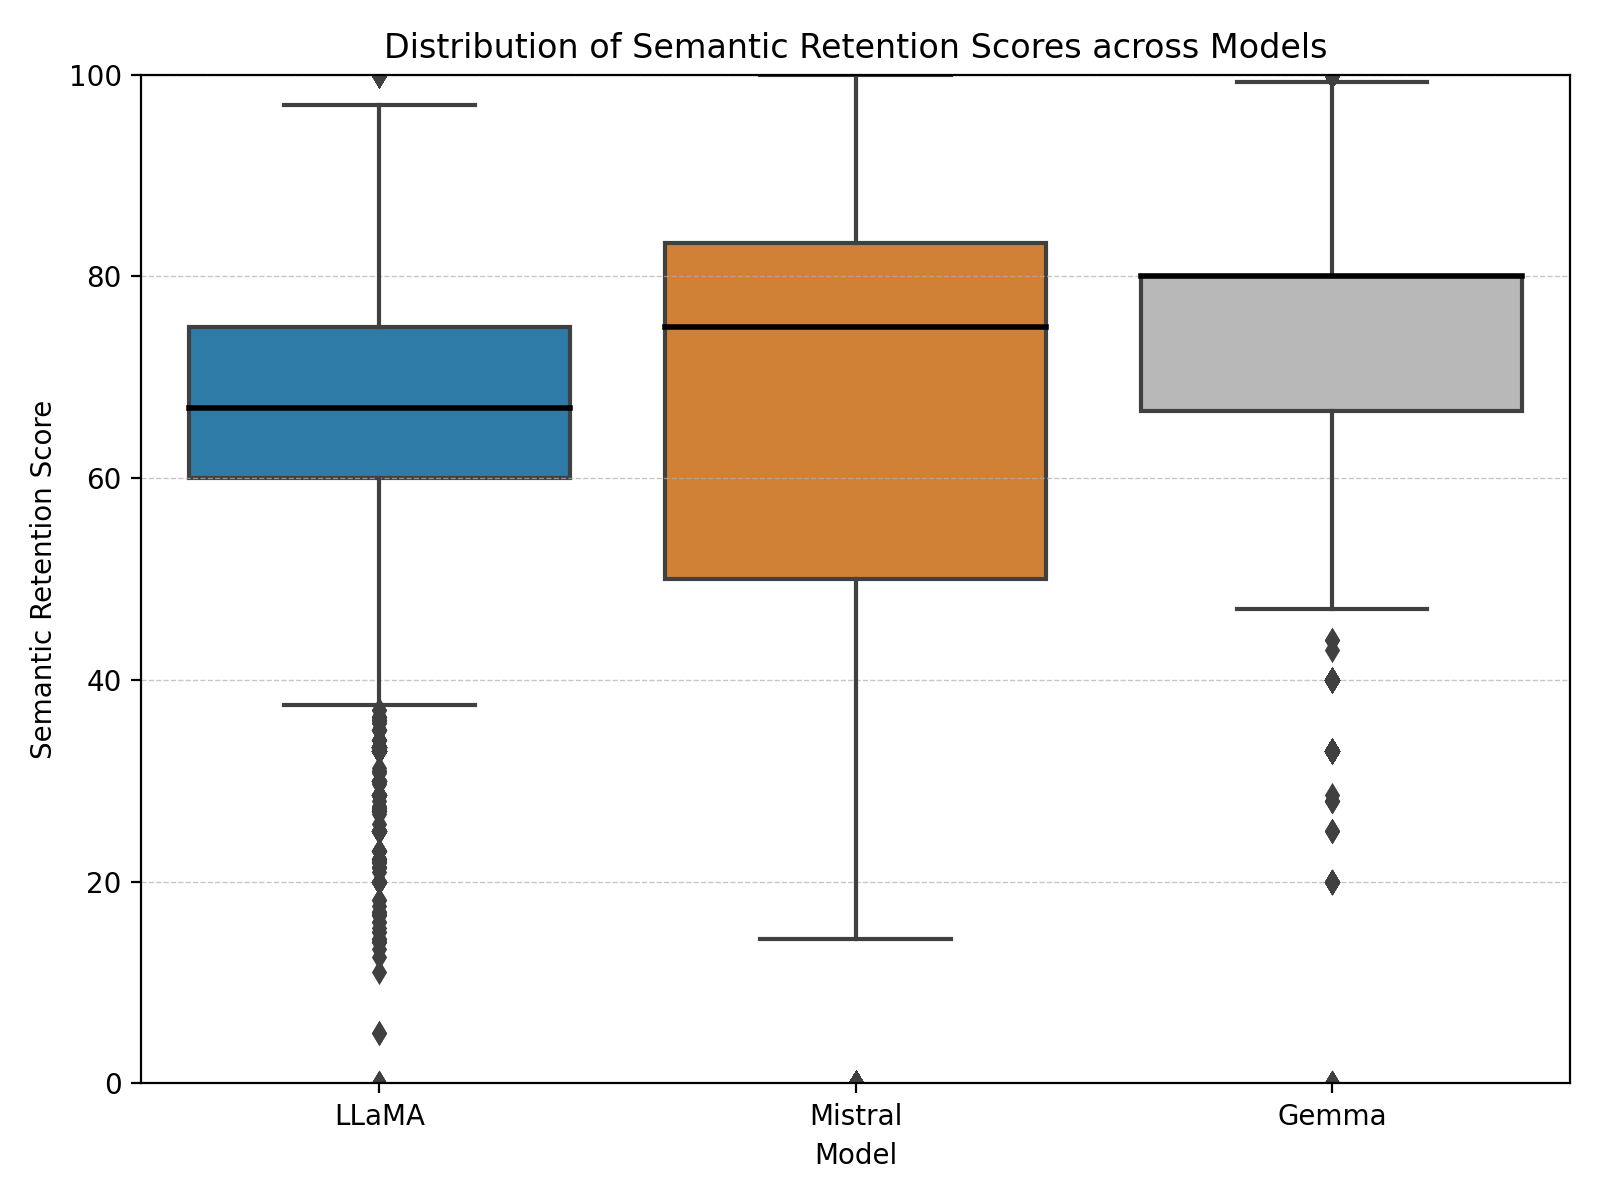
\includegraphics[width=\textwidth]{img/AvgScoresBoxplots.png}
    \caption[Distribution of semantic retention scores across models]{\textbf{Distribution of Semantic Retention Scores Across Models.} 
    The boxplot compares semantic retention scores produced by LLaMA, Mistral, and Gemma across the full dataset. LLaMA’s scores cluster around the mid-60s to low-70s with many low outliers. Mistral shows a wider distribution with higher median scores, while Gemma’s scores concentrate around the high 70s to low 80s. 
    This shows that the same article can receive different evaluations depending on the model: LLaMA tends to give lower scores, Mistral produces more variable results, and Gemma assigns consistently higher scores..}
    \label{fig:AvgScoresBoxplots}
\end{figure}

\subsection{Internal Consistency Check across LLMs}
To examine whether the language models generate semantic retention scores in a consistent and interpretable manner, we validate an internal consistency check for each model. Specifically, we compare the generated semantic retention score with an expected score derived from the number of retained and lost facts in each model’s generation. The expected score is calculated as the ratio of retained facts to the total number of listed facts, expressed as a percentage.

The correlation between the generated and expected scores serves as a proxy for internal alignment: higher correlations suggest that the model’s overall score reasonably reflects its own fact-level predictions. As shown in Figure~\ref{fig:llama_internal_consistency}, LLaMA achieves a moderate correlation (Pearson $r = 0.41$, Spearman $r = 0.37$), indicating that its generated scores follow general fact-based trends but with noticeable deviations from fact-based expectations. Gemma (Figure~\ref{fig:gemma_internal_consistency}) shows a slightly stronger alignment than LLaMA (Pearson $r = 0.44$, Spearman $r = 0.44$), capturing fact-level consistency at a comparable but somewhat higher degree. Among the three models, Mistral demonstrates the strongest internal consistency (Figure~\ref{fig:mistral_internal_consistency}), with correlation values of Pearson $r = 0.58$ and Spearman $r = 0.57$, showing the closest alignment between its reported scores and the proportions derived from its own fact lists.

As shown in \autoref{fig:AllModelOverlay} across all three models, the generated semantic retention scores tend to be higher than what would be expected from the proportion of retained to lost facts. This pattern is evident in the clustering of data points above the $y = x$ line in the scatter plots, suggesting that models systematically assign slightly inflated scores relative to their fact-based outputs. This tendency indicates that while the models capture broad semantic retention trends, they may present an overly optimistic assessment of how much information is preserved.


\begin{figure}[H]
    \centering
    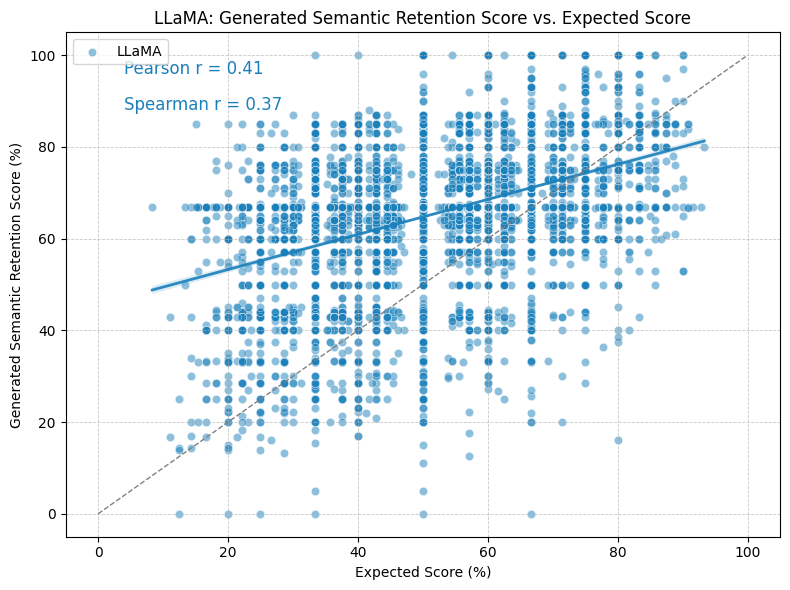
\includegraphics[width=0.8\textwidth]{img/LLaMAInternalConsistency.png}
    \caption[Internal consistency for LLaMA]{\textbf{Internal Consistency for LLaMA.} 
    The scatter plot compares LLaMA’s generated semantic retention scores with the expected scores derived from retained and lost facts. The correlation coefficients (Pearson r = 0.41, Spearman r = 0.37) indicate a moderate positive relationship, showing that the model’s outputs are moderately consistent with fact-based scores.}
    \label{fig:llama_internal_consistency}
\end{figure}

\begin{figure}[H]
    \centering
    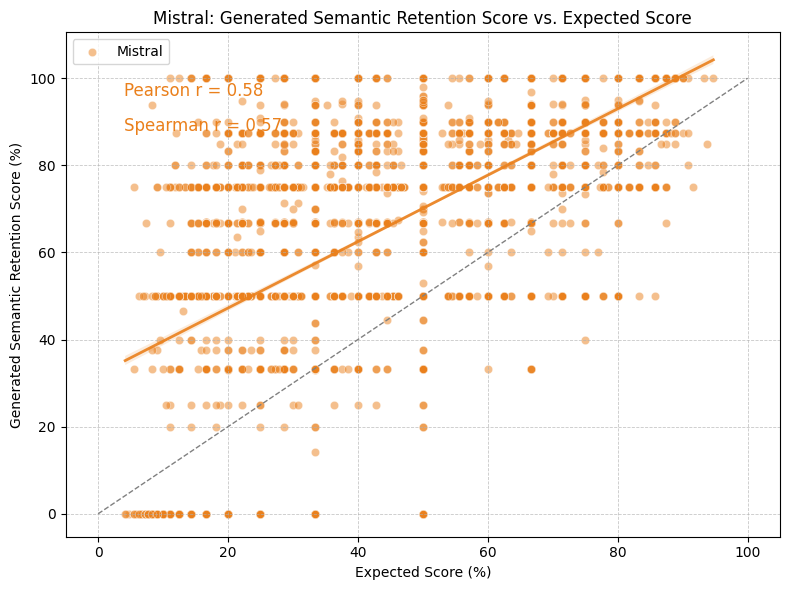
\includegraphics[width=0.8\textwidth]{img/MistralInternalConsistency.png}
    \caption[Internal consistency for Mistral]{\textbf{Internal Consistency for Mistral.} 
    The scatter plot shows Mistral’s generated semantic retention scores against expected scores. With stronger correlation values (Pearson r = 0.58, Spearman r = 0.57), Mistral demonstratesindicate a stronger positive relationship compared to LLaMA, showing that the model’s outputs are more consistent with fact-based scores.}
    \label{fig:mistral_internal_consistency}
\end{figure}

\begin{figure}[H]
    \centering
    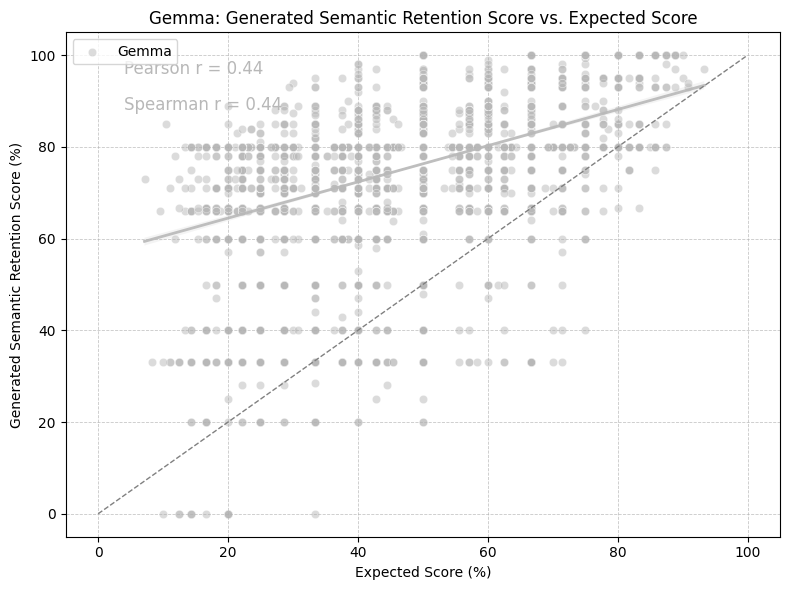
\includegraphics[width=0.8\textwidth]{img/GemmaInternalConsistency.png}
    \caption[Internal consistency for Gemma]{\textbf{Internal Consistency for Gemma.} 
    The scatter plot compares Gemma’s generated semantic retention scores with expected scores. The correlation coefficients (Pearson r = 0.44, Spearman r = 0.44) indicate a moderate positive relationship, showing that the model’s outputs are moderately consistent with fact-based scores, similar to LLaMA.}
    \label{fig:gemma_internal_consistency}
\end{figure}
\clearpage
To visually compare all three models simultaneously, \autoref{fig:AllModelOverlay} overlays their internal consistency plots. The figure confirms that Mistral provides the strongest alignment with fact-based expectations, while LLaMA and Gemma both show weaker but comparable patterns.

\begin{figure}[H]
    \centering
    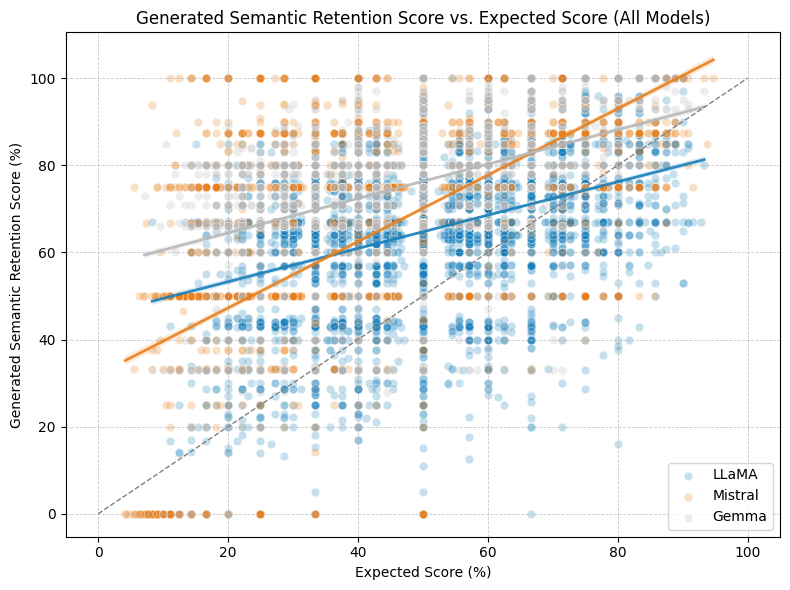
\includegraphics[width=0.75\textwidth]{img/AllModelInternalConsistency.png}
    \caption[Overlay of all models: generated vs. expected scores]{\textbf{Overlay of All Models: Generated vs. Expected Scores.} 
    The figure overlays the consistency plots of LLaMA, Mistral, and Gemma. Among the three models, Mistral shows the strongest alignment with expected scores, LLaMA shows lower consistency and often underestimates retention scores, while Gemma shows moderate consistency with relatively stable score distributions.
    This comparison shows systematic differences in how the models approximate semantic retention, indicating that model choice can influence the reliability of automated evaluation.}
    \label{fig:AllModelOverlay}
\end{figure}
\clearpage
\subsection{Human Validation}
\subsubsection{Accuracy and F1 Scores}
To assess the reliability of LLM-generated semantic retention scores and fact lists, we conduct human validation on a subset of 50 article pairs, balanced across the four main categories. For each pair, human annotators extract the ground-truth retained and lost facts, which are then compared against the LLM-generated lists to compute Accuracy and F1 scores. Accuracy measures the proportion of correctly classified facts, while the F1 score captures the balance between precision and recall. Both metrics are included to provide complementary perspectives on reliability, as F1 alone may underestimate performance in cases with few true positives.

\autoref{tab:mean_median} shows the average semantic retention scores generated by each model across the full dataset, while \autoref{tab:human_validation_results} summarizes their performance on the human-validated subset in terms of Accuracy and F1. This combined view provides an overview of both the scoring tendencies of the LLMs and how closely their fact classifications align with the human-annotated ground truth.

\begin{table}[h]
\centering
\begin{threeparttable}
\begin{tabularx}{\textwidth}{lXX}
\toprule
\textbf{Model} & \textbf{Accuracy} & \textbf{F1 Score} \\
\midrule
Random Baseline        & 0.50 & 0.33 \\
Majority Class Baseline & 0.74 & 0.00\tnote{$\S$} \\
LLaMA                  & 0.83\tnote{*,$\dag$} & 0.51\tnote{*,$\dag$} \\
Mistral                & 0.79\tnote{**,$\dag$} & 0.43\tnote{**,$\dag$,$\ddag$} \\
Gemma                  & 0.84\tnote{**,***,$\dag$} & 0.49\tnote{**,***,$\dag$} \\
\bottomrule
\end{tabularx}

\begin{tablenotes}\footnotesize
\item[*]   LLaMA fails to generate a semantic retention score for one article pair, while Mistral and Gemma succeed.
\item[**]  Both Mistral and Gemma fail to generate a semantic retention score for the same article pair.
\item[***] Gemma fails to generate a semantic retention score for one article pair, while LLaMA and Mistral succeed.
\item[$\dag$]  All models significantly outperform a random baseline classifier 
(Accuracy mean = 0.50, 95\% CI = [0.44, 0.56]; 
F1 mean = 0.33, 95\% CI = [0.26, 0.40]; 
$p < 0.01$).
\item[$\ddag$]  For Mistral, the improvement over random is smaller on F1 (p = 0.0021) but still significant.
\item[$\S$] The majority class (Lost, 219 vs. Retained, 79) yields high accuracy (0.74) but an F1 of 0.0, since it predicts no positive (Retained) cases.
\end{tablenotes}
\caption{Accuracy and F1 scores of baselines and LLMs on the human validation subset.}
\label{tab:human_validation_results}
\end{threeparttable}
\end{table}

To provide a lower-bound reference point, we additionally implement a random baseline classifier. For each article pair in the 50-sample human validation subset, the baseline randomly assigns each fact in the human-annotated ground truth list as either \textit{Retained} or \textit{Lost}. The predictions are then compared against the actual human annotations to compute Accuracy and F1 scores, yielding expected baseline values of 0.50 and 0.33, respectively. This baseline establishes how well a model would perform by chance alone, and allows us to assess whether LLMs provide a significant improvement over random guessing.

In addition, we implement a majority class baseline, which always predicts the most frequent class observed in the human validation subset. Since the majority of facts are labeled as \textit{Lost} (219 vs.\ 79 \textit{Retained}), this classifier achieves relatively high Accuracy (0.74) by predicting all facts as \textit{Lost}. However, because it never predicts any \textit{Retained} cases, its F1 score is 0.0. This baseline reflects a trivial strategy that exploits class imbalance: it achieves relatively high accuracy by always predicting the majority class, but fails to capture meaningful distinctions between retained and lost facts, resulting in an F1 score of 0.0.

As shown in \autoref{tab:human_validation_results}, all three models significantly outperform those baselines, demonstrating that their outputs capture meaningful patterns in fact retention and loss rather than those baselines.

With respect to details of results, on average, all three models achieve relatively high accuracy scores, ranging from 0.79 to 0.84. Furthermore, the results reveal distinct tendencies across the three models. Gemma consistently produces the highest average semantic retention scores and also achieves the strongest overall accuracy, suggesting that it captures a large portion of human-identified information, though it tends to assign higher scores than what might be required. LLaMA, in contrast, generates lower average scores but gets the highest F1 values, indicating a more conservative scoring behavior that nevertheless aligns more closely with human annotations at the fact level. Mistral shows the lowest performance among the three models in both accuracy and F1, reflecting greater variability and weaker alignment with human judgments. These differences highlight distinct model behaviors: Gemma emphasizes broad coverage of retained information, LLaMA balances precision and recall at the fact level, and Mistral shows comparatively lower consistency in aligning with human annotations.

A more detailed analysis of the alignment between LLM outputs and human judgments is provided in Section~\ref{sec:alignment_llm_human}.

\subsubsection{Inter-Annotator Agreement}
In addition to validating model predictions especially only LLaMA against human annotations, we also examine the consistency of the human annotations themselves. Inter-annotator agreement provides an upper bound on the reliability of the evaluation framework, since disagreement among annotators indicates inherent ambiguity in fact extraction or labeling. We measure agreement using Fleiss' $\kappa$, which accounts for chance agreement and is widely used for categorical annotation tasks. 

\autoref{tab:iaa_results} summarizes the agreement values across the four article pairs selected for detailed validation. Overall agreement is high, with an average $\kappa$ of 0.88, which corresponds to \textit{almost perfect agreement} according to the scale of Landis and Koch (1977)\cite{landis1977measurement}. Agreement is perfect ($\kappa=1.0$) for articles with concrete geographical content such as \textit{Wissignicourt} and \textit{Geelong}, reflecting their unambiguous factual nature.
By contrast, the \textit{Jackie Robinson} article yields lower agreement ($\kappa \approx 0.56$). A closer inspection shows that disagreement mainly arises from differences in granularity when interpreting complex facts. For example, the fact “He broke the color line when he started at first base” can be judged as \textit{Lost} if the annotator focuses on the specific detail of “first base”, which is absent in the simplified text, but as \textit{Retained} if the focus is on the broader notion of “breaking the color line,” which is preserved. Similarly, the fact “There was racial segregation in professional baseball” was labeled differently depending on whether annotators considered indirect mentions (e.g., references to the Negro Leagues) as sufficient evidence of retention. 
For \textit{Heat capacity}, all annotators assigned the same label to both facts, resulting in perfect agreement but an undefined $\kappa$ due to zero variance in the label distribution. Importantly, the overall agreement remained stable regardless of whether my annotations as the thesis author are included ($\kappa=0.8803$ with five annotators) or excluded ($\kappa=0.8807$ with four annotators), indicating that my role as an annotator did not affect the results.

\begin{table}[h]
\centering
\begin{threeparttable}
\begin{tabularx}{\textwidth}{lXXX}
\toprule
\textbf{Article} & \textbf{Facts (n)} & \textbf{Annotators (n)} & \textbf{Fleiss' $\kappa$} \\
\midrule
Jackie Robinson  & 6 & 5 & 0.57 \\
Wissignicourt    & 3 & 5 & 1.00 \\
Geelong          & 6 & 5 & 1.00 \\
Heat capacity    & 2 & 5 & NaN\tnote{*} \\
\midrule
Overall          & 17 & 5 & 0.88 \\
\bottomrule
\end{tabularx}

\begin{tablenotes}\footnotesize
\item[*] All annotators assigned the same label, resulting in perfect agreement but undefined $\kappa$ due to zero variance.
\end{tablenotes}
\end{threeparttable}
\caption{Inter-annotator agreement measured by Fleiss' $\kappa$ across four representative article pairs.}
\label{tab:iaa_results}
\end{table}

\vspace{-1.2em}
\subsection{Alignment Between LLMs and Human Judgments}
\label{sec:alignment_llm_human}
\vspace{-1em}
To evaluate the reliability of the proposed framework, we examine the extent to which the fact classifications generated by the LLMs align with human-annotated ground truth. Alignment is measured both quantitatively, through accuracy and F1 scores, and qualitatively, by analyzing patterns of agreement and disagreement between the models and human annotators \autoref{sec:case_study}.
Overall, the high accuracy values show that the models often agree with human annotations on whether facts are retained or lost. For example, Gemma and LLaMA both reach an accuracy above 0.83, showing frequent alignment with human judgments. At the same time, their lower F1 scores indicate that this agreement is not consistent across all facts: many human-annotated retained facts are either not listed or incorrectly classified by the models. This shows that relying on semantic retention scores alone may not give reliability, underscoring the importance of including human-validated metrics such as accuracy and F1 for a more robust assessment.

\indent\textbf{Comparison with Human-Annotated Expected Scores.}
To gain further insight into model alignment, we compare the expected semantic retention scores derived from human-annotated retained and lost fact lists with the scores calculated from the model-generated lists. For each article pair, we compute the human-annotated expected score as the proportion of retained facts among all annotated facts, and similarly calculate the model's expected score based on its generated lists. This comparison reveals how closely the models’ own fact-level predictions align with human judgments. As shown in Figures~\ref{fig:llama_human_expected}, \ref{fig:mistral_human_expected}, and \ref{fig:gemma_human_expected}, all three models show moderate correlation with human expectations. LLaMA achieves a Pearson correlation of $r = 0.44$ and Spearman $r = 0.40$ (Figure~\ref{fig:llama_human_expected}), while Mistral reaches Pearson $r = 0.44$ and Spearman $r = 0.37$ (Figure~\ref{fig:mistral_human_expected}). Gemma records Pearson $r = 0.42$ and Spearman $r = 0.47$ (Figure~\ref{fig:gemma_human_expected}).

\begin{figure}[H]
    \centering
    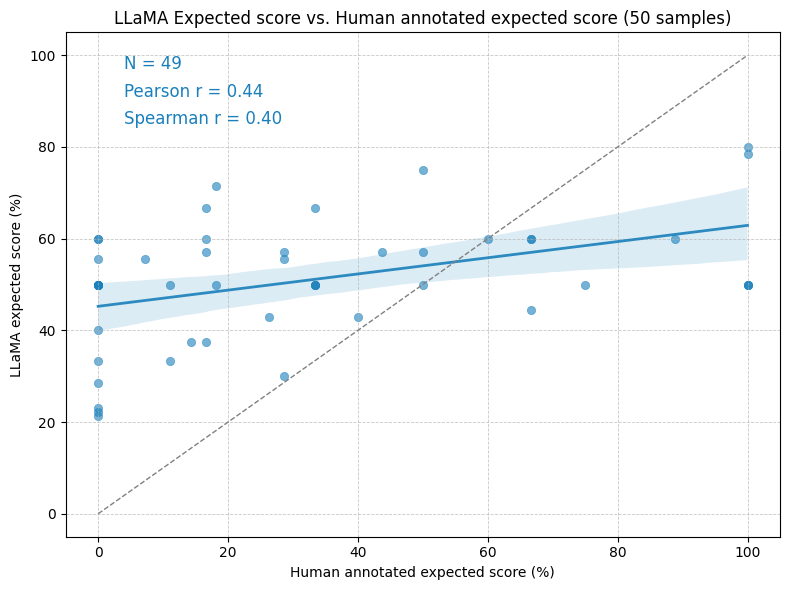
\includegraphics[width=0.75\textwidth]{img/LLaMAHumanExpectedScore.png}
    \caption[Correlation between human and model-generated expected scores for LLaMA]{\textbf{Correlation Between Human and Model-Generated Expected Scores for LLaMA.} 
    The scatter plot shows the relationship between human-annotated expected scores and those generated expected scores by LLaMA for 50 human-validated article pairs. With Pearson r = 0.44 and Spearman r = 0.40 (N = 49), the plot indicates a moderate positive correlation. 
    This indicates that LLaMA’s expected scores are moderately correlated with the human-annotated expected scores, but also show deviations, reflecting differences between model-generated and human-annotated fact-level estimates.}
    \label{fig:llama_human_expected}
\end{figure}

\begin{figure}[H]
    \centering
    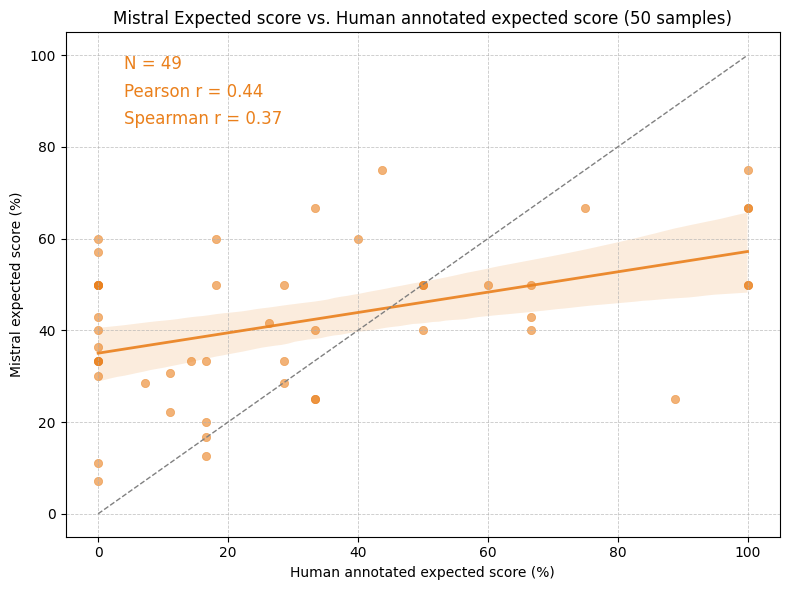
\includegraphics[width=0.75\textwidth]{img/MistralHumanExpectedScore.png}
    \caption[Correlation between human and model-generated expected scores for Mistral]{\textbf{Correlation Between Human and Model-Generated Expected Scores for Mistral.} 
    The scatter plot compares human-annotated expected scores with those produced by Mistral on the 50 human-validated article pairs. Correlation coefficients (Pearson r = 0.44, Spearman r = 0.37, N = 49) indicate a moderate alignment. 
    This shows that Mistral’s expected scores are moderately correlated with human-annotated values, but with increased spread, particularly at lower scores.}
    \label{fig:mistral_human_expected}
\end{figure}

\begin{figure}[H]
    \centering
    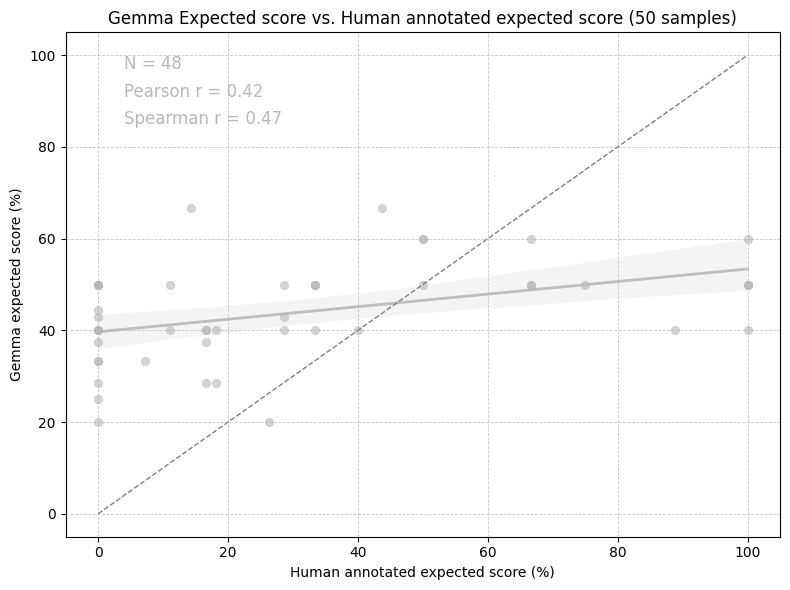
\includegraphics[width=0.75\textwidth]{img/GemmaHumanExpectedScore.png}
    \caption[Correlation between human and model-generated expected scores for Gemma]{\textbf{Correlation Between Human and Model-Generated Expected Scores for Gemma.} 
    The scatter plot compares human-annotated expected scores with those produced by Gemma on the 50-sample validation set. Correlation coefficients (Pearson r = 0.42, Spearman r = 0.47, N = 48) indicate a moderate alignment. 
    This shows that Gemma’s expected scores are moderately correlated with human-annotated values, with relatively less variability compared to Mistral but still notable differences across score levels.}
    \label{fig:gemma_human_expected}
\end{figure}

Overall, the correlations indicate that the expected scores derived from LLM-generated fact lists align with human-annotated expected scores only at a moderate level, confirming that they cannot fully substitute for human evaluation. Among the three models, LLaMA and Mistral both achieve a Pearson correlation of $r = 0.44$ with human-annotated expected scores, while Gemma reaches a similar level with $r = 0.42$. These values indicate only moderate alignment, showing that none of the models fully capture the exact proportions of retained and lost facts identified by humans. LLaMA, despite being more conservative and balanced at the fact level, does not surpass the others in terms of correlation strength. Mistral achieves the same correlation level as LLaMA but with greater variability, which reduces its consistency. Gemma, although slightly lower in Pearson correlation, remains comparable overall.

Moderate correlations ($r \approx 0.4$–$0.5$) are acceptable given the inherent difficulty of fact-level evaluation. Prior work has also found only moderate associations between automatic metrics and human judgments. For instance, Cachola et al. (2025)\cite{cachola2025evaluating} evaluated traditional readability metrics against human judgments and found a best correlation of about $r = 0.56$, suggesting that this level of alignment is consistent with broader trends in the field.

\section{Qualitative Analysis: Case Studies}
\label{sec:case_study}
To complement the quantitative findings, we provide a qualitative analysis based on case studies. 
We focus on two groups of articles: (i) \textit{High Agreement Articles Across All Models}, where LLaMA, Mistral, and Gemma all generate scores greater than their respective medians, and (ii) \textit{Low Agreement Articles Across All Models}, where all three models assign scores below their medians. 
This allows us to examine how model consensus manifests at the fact level, and whether high or low semantic retention scores correspond to actual preservation or loss of information. 
Across the 10,000 aligned article pairs, the model-specific medians were 67.0 for LLaMA, 75.0 for Mistral, and 80.0 for Gemma. 
Applying these thresholds, we identified 3,070 high-agreement articles and 1,641 low-agreement articles. 
Within the human-validated subset of 50 articles, three titles overlapped with the high-agreement group (\textit{Holliday Grainger, Noguères, The Lonely White Sail}), while several others fell into the low-agreement group. 
Representative fact-level tables are provided in Appendix \ref{appendix:casestudy}, while we summarize the main findings here.

\paragraph{High Agreement Articles Across All Models.}
Among the 3,070 high-agreement articles, three overlapped with the human-validated subset. 
For \textit{Holliday Grainger}, all models picked up the facts that were first mentioned in the English Wikipedia entry, such as her identity and her main roles. However, the facts that appeared later in the text were often omitted and marked as “not listed.” This shows that the models handle the first-mentioned information reliably but tend to lose coverage on later-mentioned details, especially when the text is written in a list format. This is reflected in the metrics (\autoref{tab:holliday_metrics}), where Mistral achieved the highest performance (Accuracy = 0.94, F1 = 0.92), followed by Gemma (Accuracy = 0.86, F1 = 0.84) and LLaMA (Accuracy = 0.81, F1 = 0.73).
In \textit{Noguères}, the simplified entry contained only two facts, which all models retained perfectly (\autoref{tab:nogueres_metrics}, Accuracy=1.0, F1=1.0), showing that short and almost identical entries across English and Simple English Wikipedia are easy for models to handle consistently.

By contrast, in the case of \textit{The Lonely White Sail}, the input also contained only two central facts, but the Simple English Wikipedia version added extra sentences compared to the English entry. Both LLaMA and Gemma captured only one fact correctly, while Mistral failed to retain either. This indicates that even very short inputs can lead to divergence when the simplified version introduces additional information. Models can still miss even the main facts, which leads to very different results across systems.

Overall, these cases illustrate that high agreement is not simply a function of input length or simplicity. When the simplified and original entries are nearly identical, as in \textit{Noguères}, perfect agreement emerges. But when simplification either enumerates many details, as in \textit{Holliday Grainger}, or introduces new content, as in \textit{The Lonely White Sail}, models begin to diverge. This highlights the importance of analyzing not only the amount of information preserved but also the structural differences between original and simplified texts to understand why agreement occurs in some cases but breaks down in others.

\paragraph{Low Agreement Articles Across All Models.}
In contrast to the high-agreement cases, the low-agreement articles highlight scenarios where all three models fall below their respective medians, often struggling to capture or correctly classify the retained information. 
We illustrate this with three examples: \textit{Black site}, \textit{Bureau of Indian Affairs} and \textit{Enhanced Geothermal Systems}.

In the case of \textit{Black site}, the human annotation identified only one retained fact, with all others classified as lost. LLaMA captured the retained fact but also hallucinated two additional retentions, reducing its precision (\autoref{tab:blacksite_llama}). Mistral labeled all facts as lost, which meant it correctly handled the majority but failed to capture the single retained fact (\autoref{tab:blacksite_mistral}). Gemma produced the closest alignment with human annotations, retaining the correct fact while marking most others as lost, though occasionally using “not listed” for lost facts (\autoref{tab:blacksite_gemma}). The aggregated results in \autoref{tab:blacksite_metrics} highlight the sharp divergence: Gemma achieved F1=1.0, LLaMA dropped to 0.50 due to false positives, and Mistral to 0.0 due to a single false negative.

For \textit{Bureau of Indian Affairs}, the simplification involved not only deletion of institutional and administrative details but also the addition of new contextual information, such as the agency’s founding year and references to the Bureau of Indian Education. Therefore, the human annotation marked only one fact as retained, with all other details classified as lost. Among the models, Mistral was the only one to capture this fact correctly, whereas both LLaMA and Gemma either marked it as “not listed” or classified it as lost, resulting in no true positives. However, Mistral also produced several false positives by incorrectly labeling many lost facts as retained, which significantly reduced its precision and led to a modest F1 score (0.26). In contrast, LLaMA and Gemma, despite avoiding hallucinated retentions, failed to recover the single retained fact, yielding F1 scores of 0.0. These results are detailed in \autoref{tab:bia_llama}, \autoref{tab:bia_mistral}, and \autoref{tab:bia_gemma}, with an aggregated summary provided in \autoref{tab:bia_metrics}.

In the case of \textit{Enhanced Geothermal Systems}, Both LLaMA and Gemma correctly identified this fact, as shown in \autoref{tab:egs_llama} and \autoref{tab:egs_gemma}, resulting in near-perfect performance. In contrast, Mistral failed to capture the single retained fact and labeled all facts as lost (\autoref{tab:egs_mistral}), which led to an F1 score of 0.0. The aggregated results in \autoref{tab:egs_metrics} illustrate this sharp divergence: while LLaMA and Gemma achieved F1 = 1.0, Mistral collapsed to F1 = 0.0. This case therefore represents a genuine low-agreement scenario, where models differ significantly in their ability to detect the few facts preserved in simplification.

Overall, these low-agreement cases show that the models do not all fail in the same way, but instead make different kinds of mistakes. In situations where only a single fact is retained or where simplification mixes deletion and addition, some models miss the retained fact, others add facts that are not present, and only a few align closely with the human annotation.

\paragraph{Model-level Agreement}
To complement the fact-level comparisons, we examine the overall agreement between models in terms of their generated semantic retention scores.
Figures \ref{fig:llama_mistral}, \ref{fig:mistral_gemma}, and \ref{fig:llama_gemma} display pairwise scatter plots with Spearman’s $\rho$ for each model pair.
The results show moderate consistency between LLaMA and Mistral ($\rho=0.40$; Figure~\ref{fig:llama_mistral}) and between LLaMA and Gemma ($\rho=0.41$; Figure~\ref{fig:llama_gemma}), while the strongest alignment is observed between Mistral and Gemma ($\rho=0.57$; Figure~\ref{fig:mistral_gemma}).

The scatter plots also show how the models differ in practice. In Figure~\ref{fig:llama_mistral}, Mistral often gives the maximum score (100) where LLaMA assigns more varied values, lowering their rank agreement. In Figure~\ref{fig:mistral_gemma}, Gemma usually assigns equal or higher scores than Mistral in high-retention cases, explaining the stronger correlation. In Figure~\ref{fig:llama_gemma}, Gemma consistently scores higher than LLaMA, reflecting its more optimistic scoring style.

Overall, the models tend to agree on which articles are generally easy or difficult, as seen in their correlated scores. But at the fact level, their predictions still different tendencies, so global score agreement does not imply detailed agreement.

\begin{figure}[H]
    \centering
    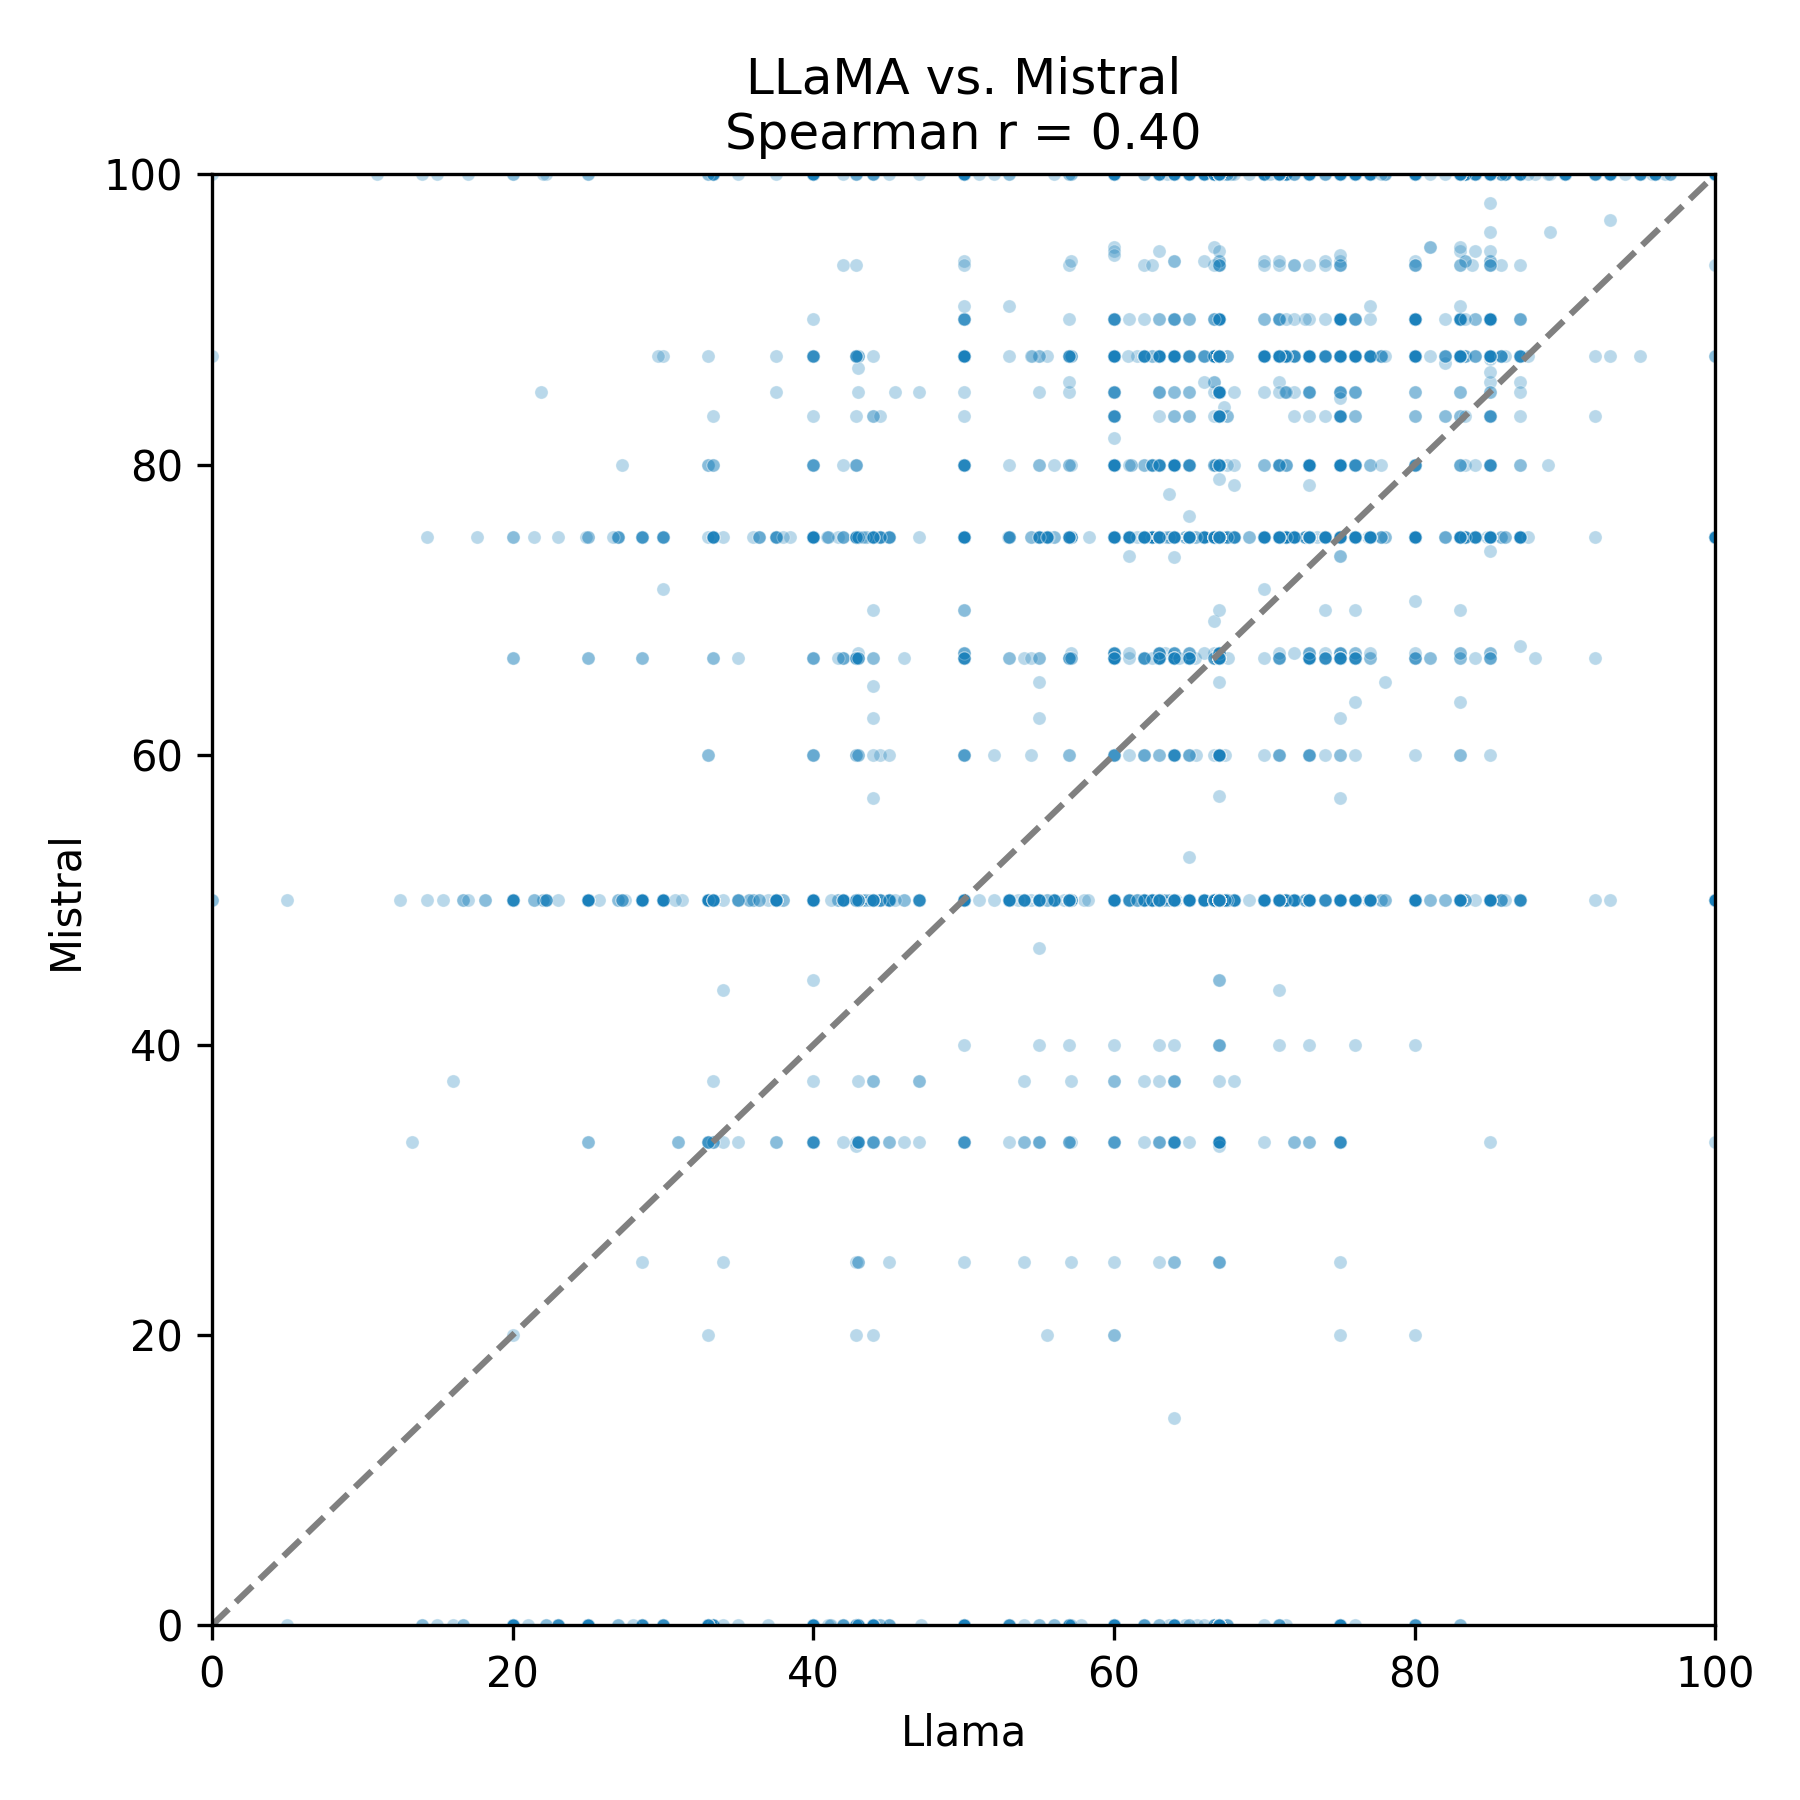
\includegraphics[width=0.75\textwidth]{img/llama_mistral.png}
    \caption[Rank correlation of semantic retention scores between LLaMA and Mistral]{\textbf{Rank Correlation of Semantic Retention Scores Between LLaMA and Mistral.} 
    The scatter plot compares semantic retention scores from LLaMA and Mistral across the full dataset. The Spearman rank correlation of $r = 0.40$ indicates a moderate positive relationship. 
    This suggests that while the two models share some agreement in ranking article-level retention, their predictions often diverge, highlighting differences in how each model interprets retained and lost information.}
    \label{fig:llama_mistral}
\end{figure}

\begin{figure}[H]
    \centering
    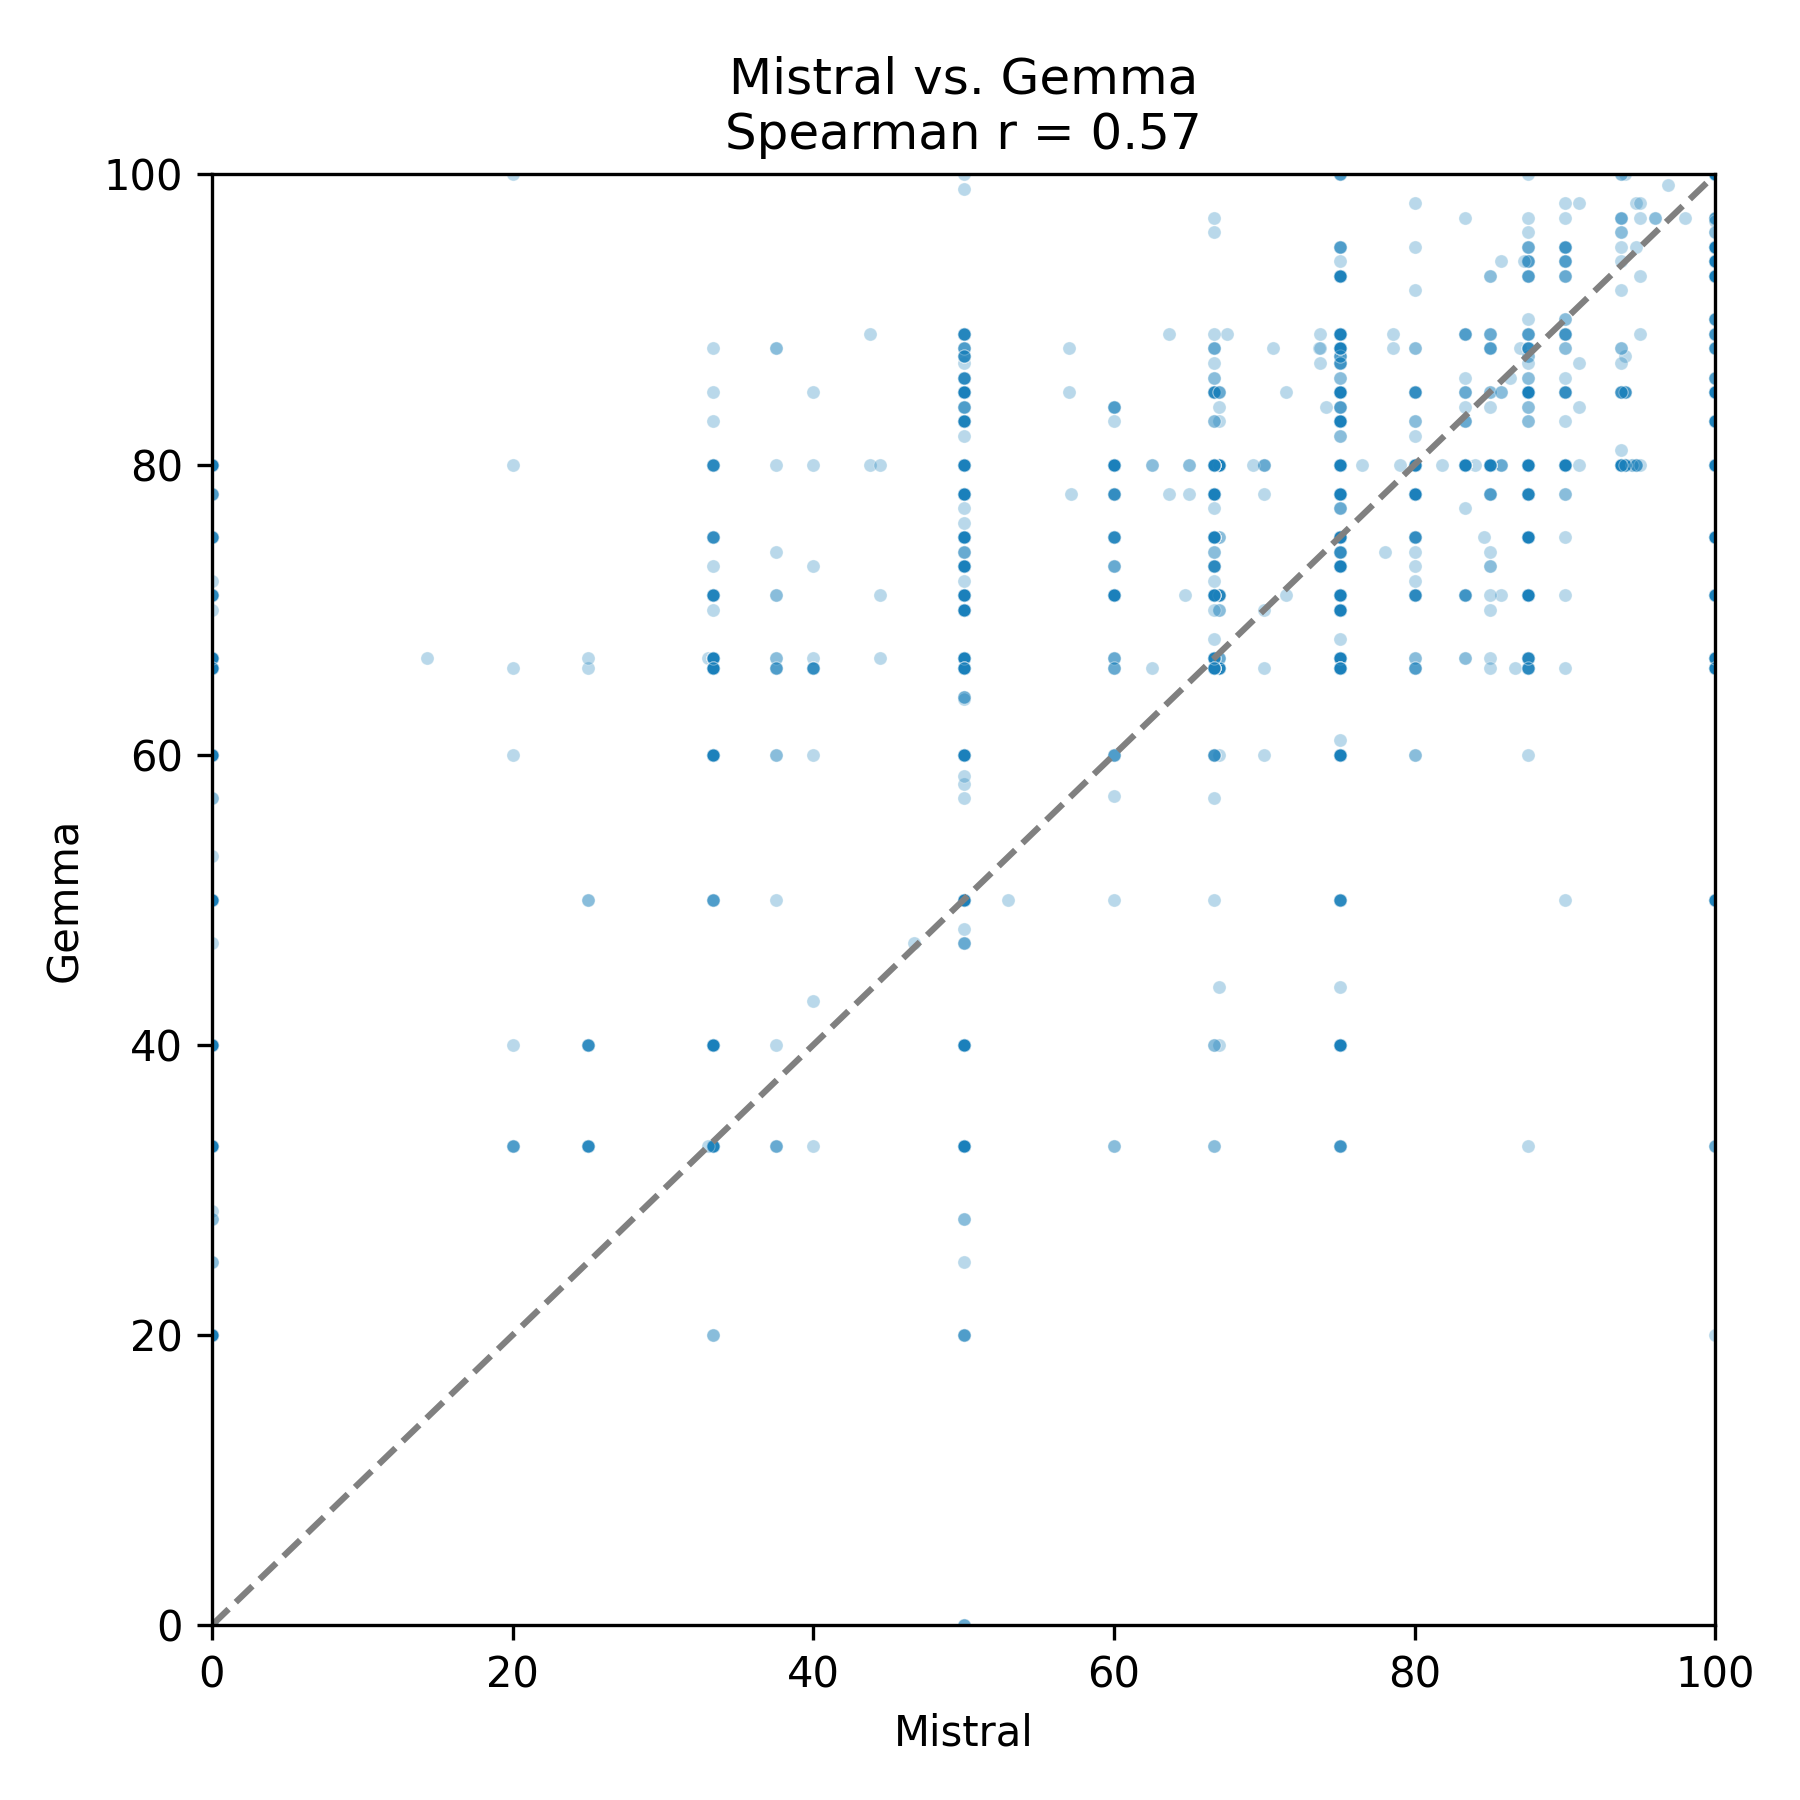
\includegraphics[width=0.75\textwidth]{img/mistral_gemma.png}
    \caption[Rank correlation of semantic retention scores between Mistral and Gemma]{\textbf{Rank Correlation of Semantic Retention Scores Between Mistral and Gemma.} 
    The scatter plot shows the comparison of semantic retention scores between Mistral and Gemma. The Spearman rank correlation of $r = 0.57$ is the strongest among model pairs, indicating relatively high agreement. 
    This suggests that Mistral and Gemma share more similar scoring behavior, particularly in ranking articles with higher retention scores, compared to LLaMA.}
    \label{fig:mistral_gemma}
\end{figure}

\begin{figure}[H]
    \centering
    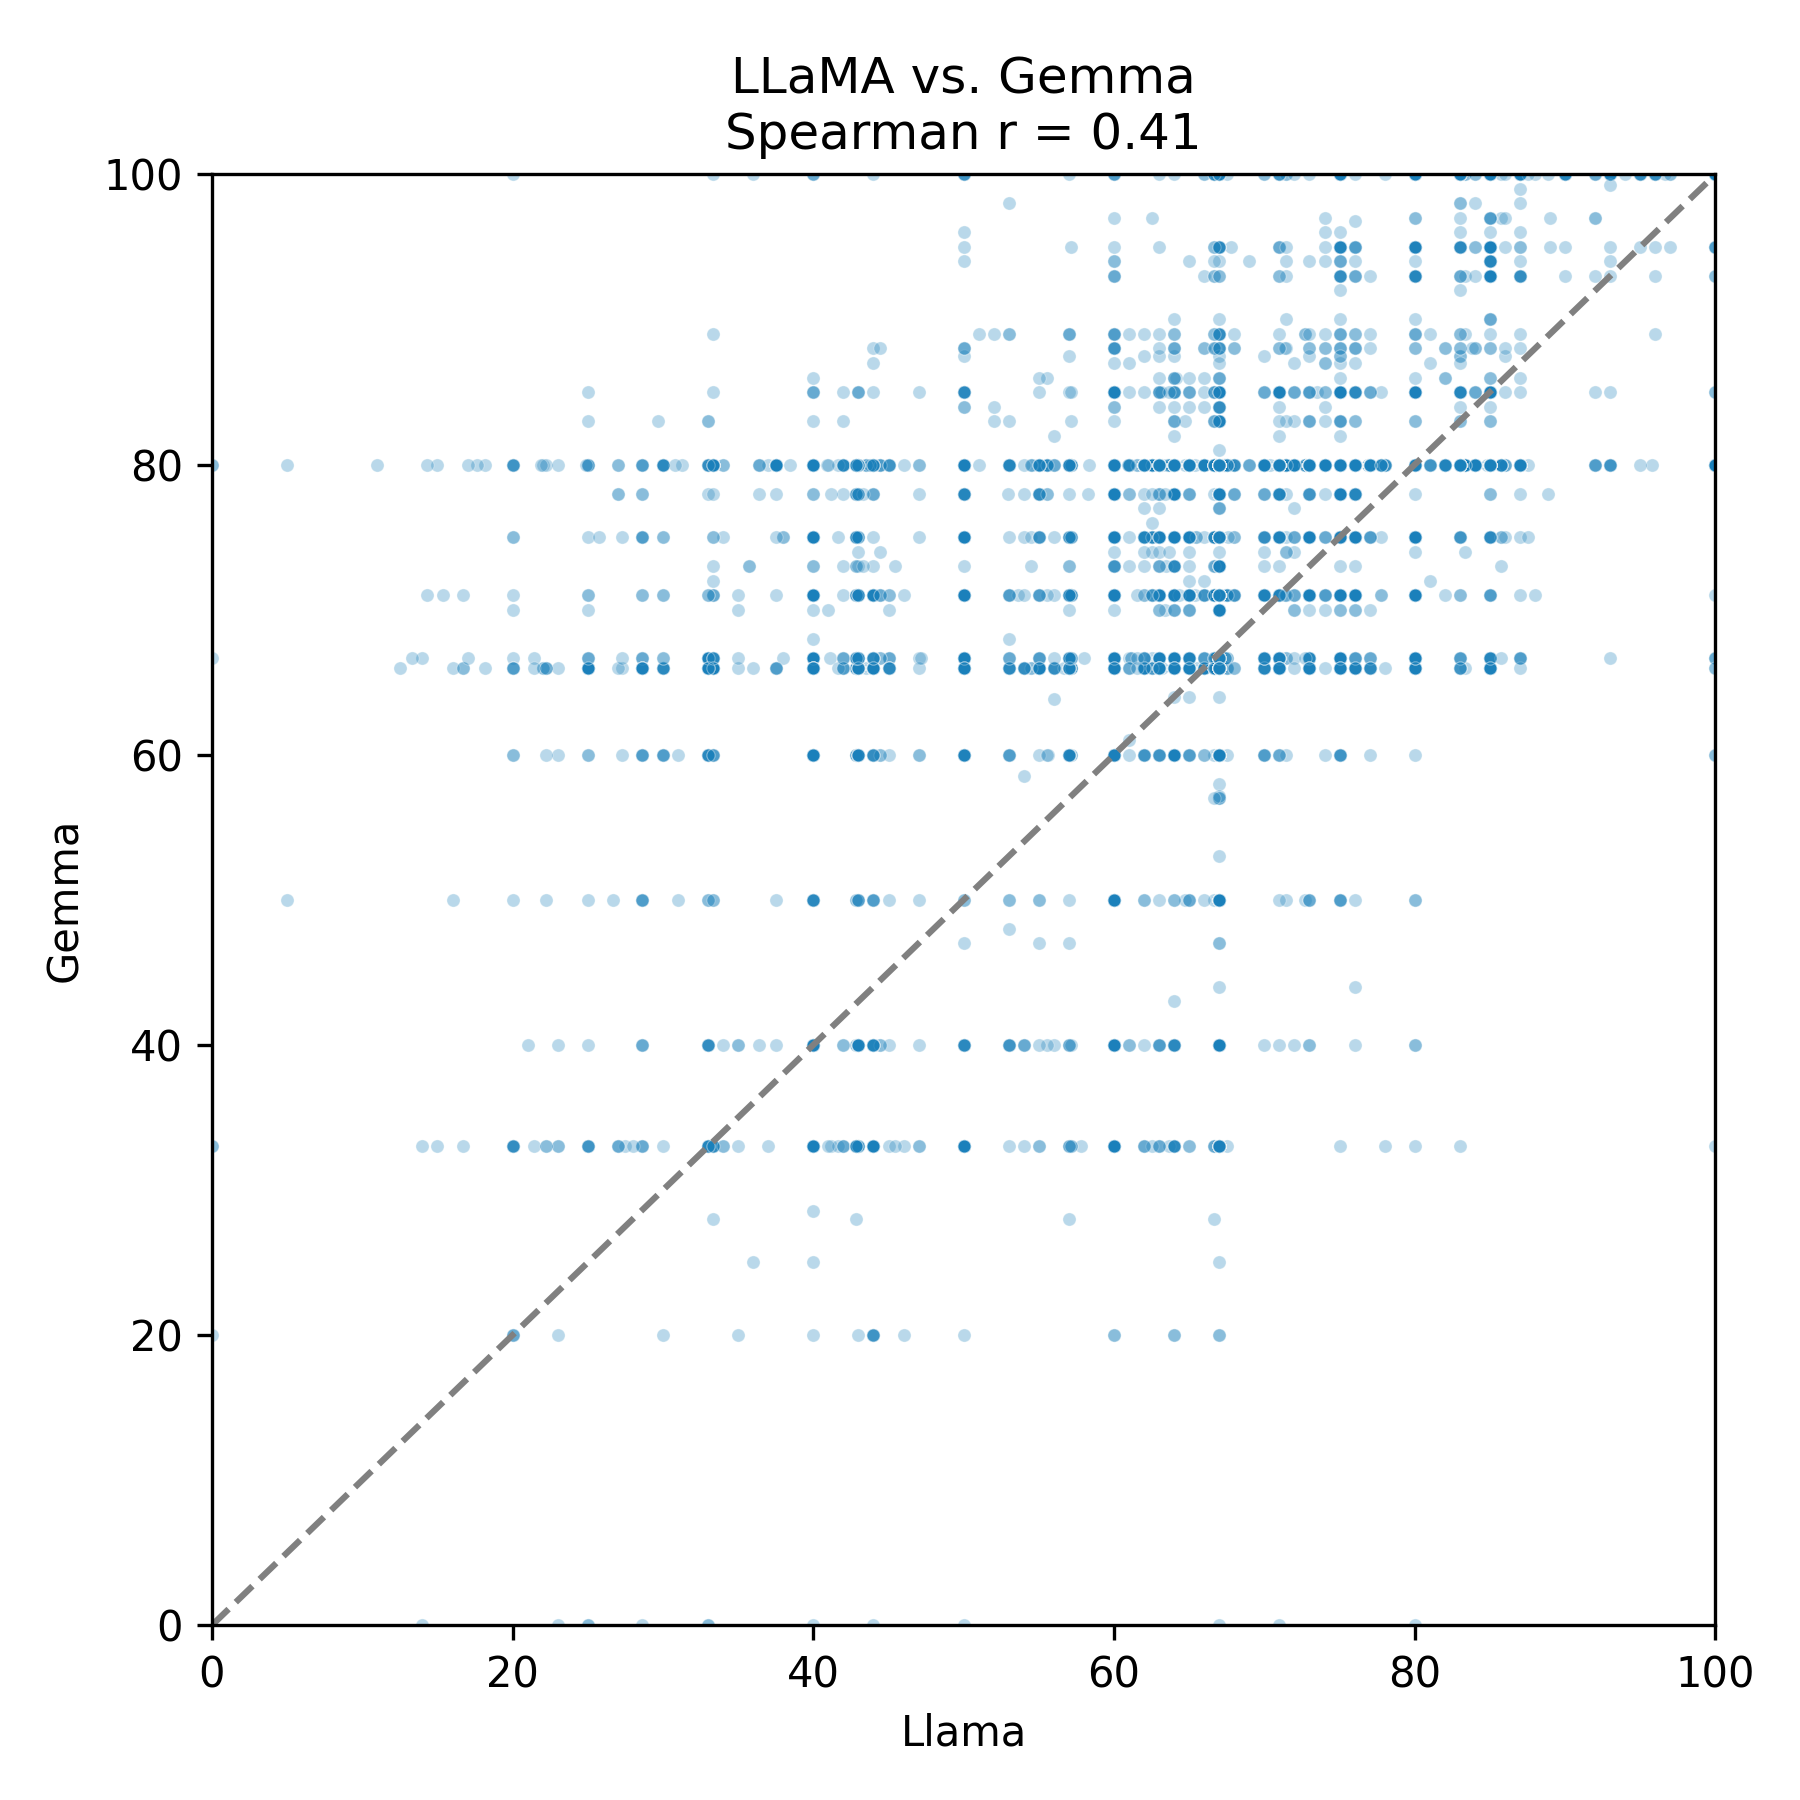
\includegraphics[width=0.75\textwidth]{img/llama_gemma.png}
    \caption[Rank correlation of semantic retention scores between LLaMA and Gemma]{\textbf{Rank Correlation of Semantic Retention Scores Between LLaMA and Gemma.} 
    The scatter plot compares semantic retention scores assigned by LLaMA and Gemma. The Spearman rank correlation of $r = 0.41$ indicates moderate alignment. 
    This result shows that while Gemma provides more stable retention estimates overall, its rankings do not fully converge with LLaMA, underscoring systematic differences in their evaluation of retained vs. lost facts.}
    \label{fig:llama_gemma}
\end{figure}

\clearpage
\section{Research Goal 2: Which Topics Show Higher Information Loss?}
\subsection{Topic-wise Retention and Loss Patterns (10k Dataset)}
Based on the ORES-predicted fine-grained topics (e.g., \texttt{Culture.Biography, Culture.Media, Culture.Sports}), we merge related labels into four broader main categories: Culture, Geography, History and Society, and STEM. Using these aggregated categories, we analyze the average semantic retention scores in the 10k dataset to identify topic-specific patterns of information loss.

\autoref{tab:AvgCategoryScores} shows the average semantic retention scores across all models for each main category. The results reveal clear topic-dependent variation. Culture and Geography articles obtain the highest average scores (69.86 and 69.69, respectively), indicating that these categories tend to preserve more information during simplification compared to History and Society or STEM. By contrast, History and Society (65.35) and STEM (64.81) record lower averages, indicating that terminology-heavy domains and technical content are more prone to information loss.

To examine model across different topics, a more fine-grained view is provided in \autoref{tab:CategoryModelScores} and \autoref{fig:AvgScoresCategory} , which reports model-specific retention and loss values per category. In particular, \textbf{Gemma} consistently achieves the highest semantic retention across all domains. For instance, 75.49\% in Geography (24.51\% loss) and 72.65\% in STEM (27.35\% loss). By contrast, \textbf{Mistral} assigns lower score in complex domains, retaining only 59.96\%(40.04\% loss)  in History and Society and 57.76\% (42.24\% loss)in STEM. \textbf{LLaMA} generally falls between the two, with retention around 64-66\% depending on the category. Taken together, these results confirm that simplification-induced information loss is highly domain-dependent, with STEM and History consistently emerging as the most challenging categories, and also reveal substantial performance gaps between models in these categories.  

Given that the automated assessment using LLMs demonstrates reasonably reliable through human validation, we observe that technical domains, especially STEM tend to suffer greater information loss during the simplification process.

\begin{table}[H]
\centering
\caption{Average semantic retention by category, aggregated across the three models (valid outputs only).}
\label{tab:AvgCategoryScores}
\begin{tabular}{lc}
\toprule
Main Category & Mean (across LLaMA, Mistral, Gemma) \\
\midrule
Culture                & 69.86 \\
Geography              & 69.69 \\
History and Society    & 65.35 \\
STEM                   & 64.81 \\
\bottomrule
\end{tabular}
\end{table}

\begin{table}[H]
\centering
\caption{Average semantic retention by category and model (valid outputs only).}
\label{tab:CategoryModelScores}
\begin{tabular}{lccc}
\toprule
Main Category & LLaMA & Mistral & Gemma \\
\midrule
Culture                & 65.68 & 68.43 & 75.47 \\
Geography              & 66.10 & 67.48 & 75.49 \\
History and Society    & 63.67 & 59.96 & 72.43 \\
STEM                   & 64.01 & 57.76 & 72.65 \\
\bottomrule
\end{tabular}
\end{table}

\begin{figure}[H]
    \centering
    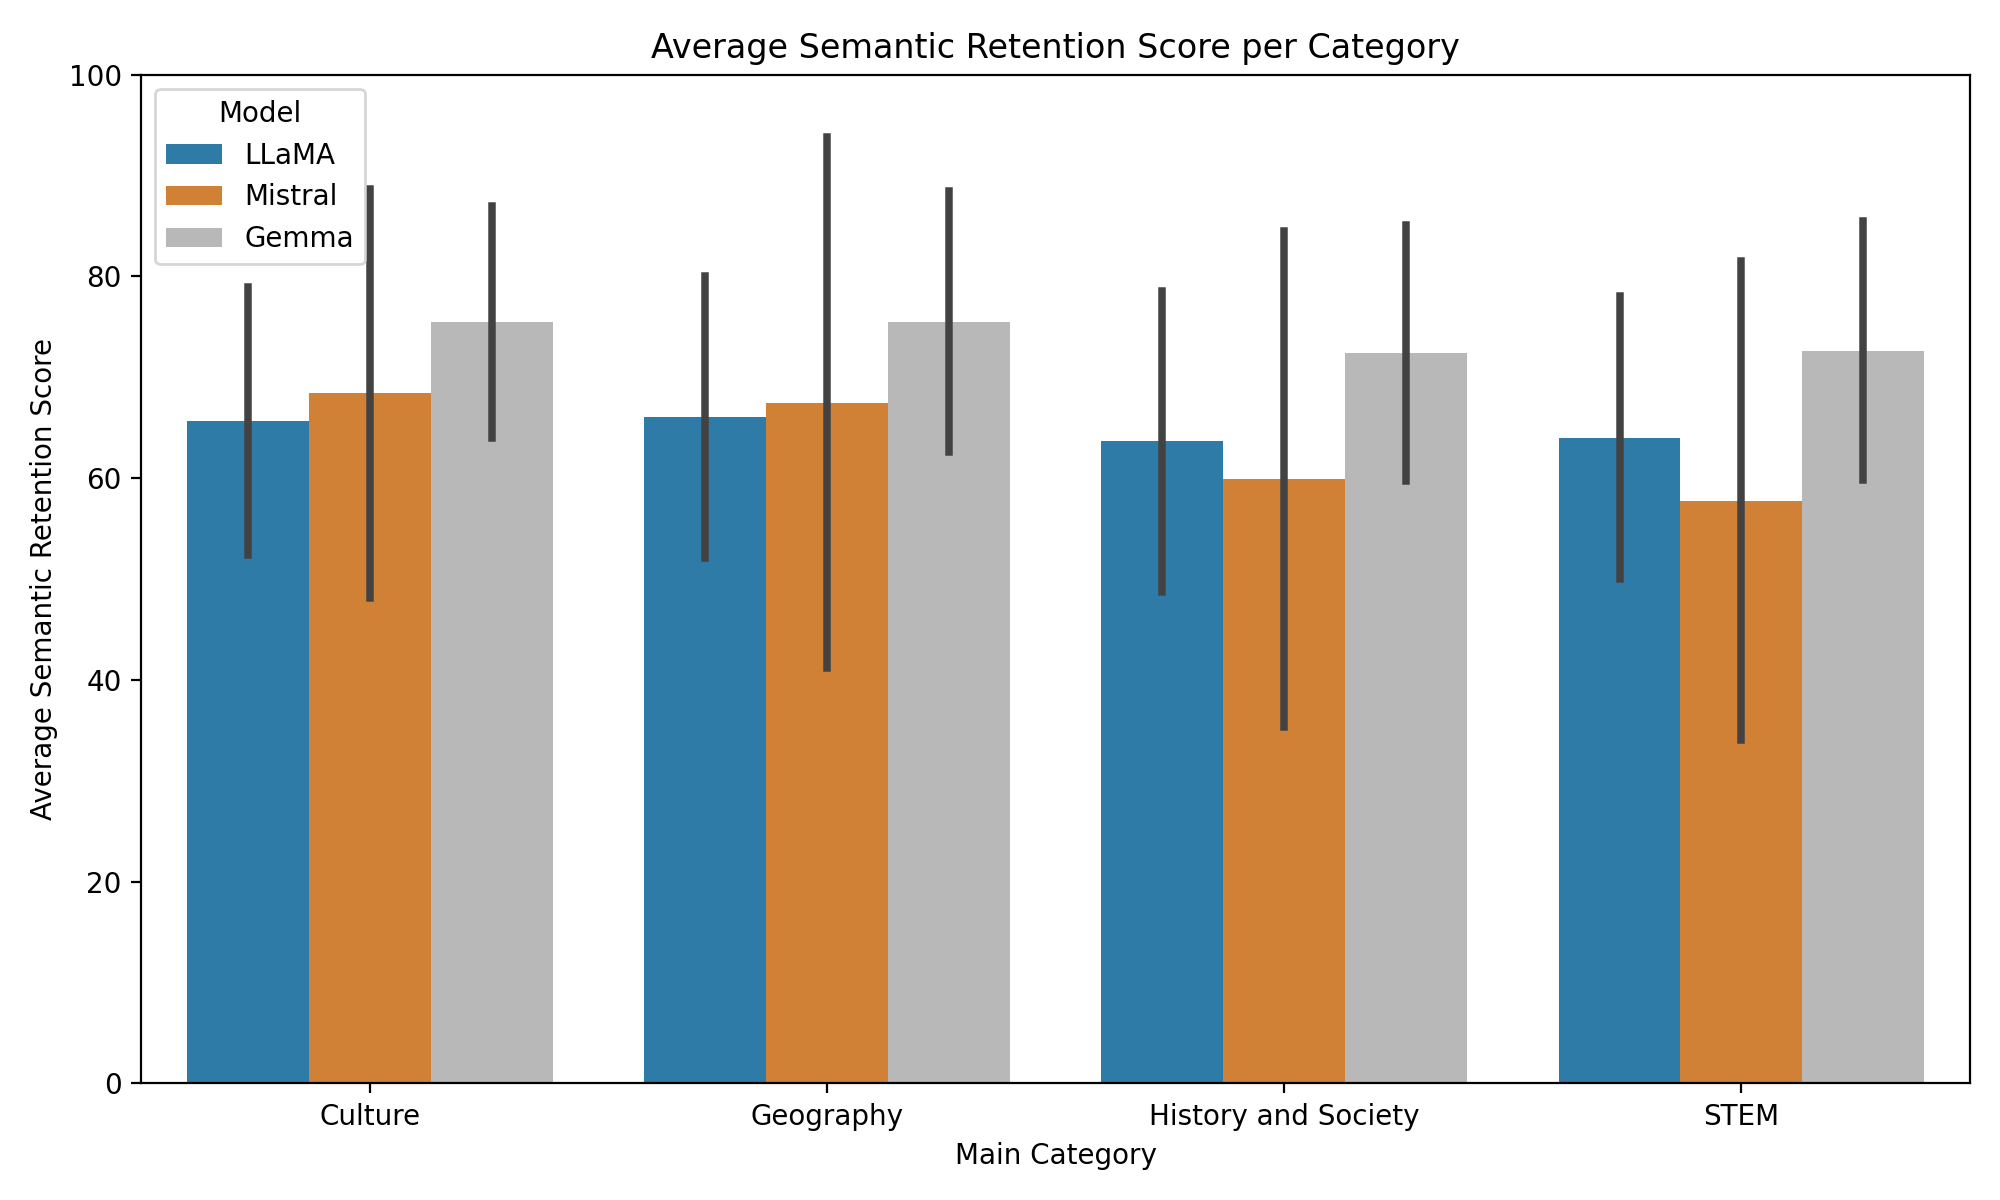
\includegraphics[width=1.0\textwidth]{img/AvgScoresCategory.png}
    \caption[Average semantic retention scores per category and model]{\textbf{Average Semantic Retention Scores per Category and Model.} 
    The bar chart displays the average semantic retention scores across four main categories (Culture, Geography, History and Society, STEM) for LLaMA, Mistral, and Gemma. Error bars indicate score variability within each category. 
    The bar chart shows the average semantic retention scores across four main categories (Culture, Geography, History and Society, STEM) for LLaMA, Mistral, and Gemma. Error bars indicate within-category variability. Gemma has the highest average score in all categories. Mistral generates higher scores than LLaMA in Culture and Geography, whereas LLaMA produces higher than Mistral in History and Society and STEM. These results show that the relative ranking of models varies by domain
    This comparison highlights that differences in model performance are not uniform across domains, suggesting that topic-specific characteristics influence how well semantic information is retained during simplification.}
    \label{fig:AvgScoresCategory}
\end{figure}.

\subsection{Topic-wise Accuracy and F1 Scores}
These category-level patterns are also reflected in the human validation results (\autoref{tab:CategoryModelValidation}) across all models, confirming that information loss varies across topics. Overall, STEM and History and Society emerge as the most challenging categories, while Culture and Geography show comparatively stronger alignment with human annotations.

For STEM, although the average retention percentages are not the lowest across models (e.g., Gemma 72.65\%), the human-validated F1 scores are by far the lowest (LLaMA 0.15, Mistral 0.19, Gemma 0.29). This indicates that the models often struggle to correctly determine which specific technical facts are preserved or omitted. Consequently, retention percentages in STEM can be misleading, as they obscure frequent errors in fact-level classification. History and Society shows a similar difficulty: retention scores are lower than in Culture or Geography (e.g., Mistral 59.96\%), and F1 scores remain relatively low (LLaMA 0.41, Mistral 0.33, Gemma 0.39). The nuanced and terminology-heavy domains makes fact extraction and alignment particularly challenging.

In contrast, Culture and Geography assigns semantic retention score higher than the others overall. Culture achieves consistently higher F1 scores (e.g., up to 0.76 for LLaMA), reflecting that biographical and descriptive entries allow models to preserve key facts with greater accuracy. Geography also attains relatively strong F1 values (0.58-0.71 across models), but it records the lowest accuracy values in some cases (e.g., 0.61 for Mistral, 0.72 for LLaMA). This suggests that while the models capture many individual facts correctly, a smaller number of misclassifications has a disproportionate effect on overall agreement.

Overall, these findings highlight the importance of considering both F1 and accuracy when evaluating model performance. F1 is more sensitive to the correctness of individual fact identification, whereas accuracy reflects overall agreement with human labels. Both metrics are needed to capture the different ways models succeed or fail across categories, with STEM and History and Society consistently showing the greatest vulnerability to information loss.

\begin{table}[H]
\centering
\caption{Per Category and Per Model - Semantic Retention Scores (10k) and Human Validation Accuracy/F1 (50 samples)}
\label{tab:CategoryModelValidation} 
\begin{threeparttable}
\resizebox{\textwidth}{!}{%
\begin{tabular}{l|ccc|ccc|ccc}
\toprule
\textbf{Category} & \multicolumn{3}{c|}{\textbf{Retention Score (\%)}} & \multicolumn{3}{c|}{\textbf{Accuracy}} & \multicolumn{3}{c}{\textbf{F1 Score}} \\
 & \textbf{LLaMA} & \textbf{Mistral} & \textbf{Gemma} & \textbf{LLaMA} & \textbf{Mistral} & \textbf{Gemma} & \textbf{LLaMA} & \textbf{Mistral} & \textbf{Gemma} \\
\midrule
Culture              & 65.68 & 68.67 & 75.47 & 0.91 & 0.82 & 0.88\tnote{*} & 0.76 & 0.58 & 0.59\tnote{*} \\
Geography            & 66.25 & 67.48 & 75.49 & 0.72\tnote{**} & 0.61\tnote{***} & 0.81\tnote{***} & 0.71\tnote{**} & 0.58\tnote{***} & 0.70\tnote{***} \\
History and Society  & 63.67 & 59.96 & 72.43 & 0.86 & 0.83 & 0.89 & 0.41 & 0.33 & 0.39 \\
STEM                 & 64.01 & 57.76 & 72.65 & 0.81 & 0.90 & 0.80 & 0.15 & 0.19 & 0.29 \\
\bottomrule
\end{tabular}%
}
\begin{tablenotes}\footnotesize
\item[*]   Gemma fails to generate a semantic retention score for one article pair, while LLaMA and Mistral succeed.
\item[**]  LLaMA fails to generate a semantic retention score for one article pair, while Mistral and Gemma succeed.
\item[***] Both Mistral and Gemma fail to generate a semantic retention score for the same article pair.
\end{tablenotes}
\end{threeparttable}
\end{table}

\section{Summary of Key Findings}
The large-scale analysis across 10{,}000 aligned article pairs shows that the three evaluated models differ not only in their average semantic retention scores but also in their internal consistency, robustness of outputs, and alignment with human judgments. On the automatic scores alone, Gemma assigns the highest mean (75.10) and median (80.0), while Mistral and LLaMA yield lower means of 66.65 and 65.62, respectively. Median values with Mistral 75.0, Gemma 80.0, and LLaMA 67.0 indicate that Gemma and Mistral more frequently produce higher-scored outputs, whereas LLaMA’s lower median suggests a flatter distribution with more moderate scores. These distributional differences show that, although all three models can rate simplified content as highly retained, their scoring tendencies are not the same.

Robustness of the inference outputs further distinguishes the models. Mistral produces the most consistently parseable responses, with only a small number of invalid cases overall (e.g., few missing or out-of-range values), Gemma shows no out-of-range scores but a larger number of missing values than Mistral, and LLaMA shows the highest count of missing values and a small number of out-of-range scores. Thus, robustness at scale depends not only on how high scores are on average but also on how reliably models return usable, well-formed outputs.

Internal consistency checks add another perspectives. Comparing each model’s reported semantic retention score with the expected score computed from its own retained and lost fact lists yields moderate alignment for LLaMA (Pearson $r=0.41$, Spearman $r=0.37$) and Gemma (Pearson $r=0.44$, Spearman $r=0.44$), with Mistral showing the strongest internal consistency (Pearson $r=0.58$, Spearman $r=0.57$). This indicates that Mistral’s scalar scores most closely track the proportions implied by its own fact lists. At the same time, all models tend to overestimate retention relative to their fact counts, with many points lying above the $y{=}x$ line. The semantic retention scores are therefore informative in aggregate but should be interpreted together with fact-level evidence.

A topic-level breakdown reveals systematic patterns in where information loss is most likely. Culture and Geography display higher average scores across models, while History and Society and especially STEM are consistently lower. In these latter topics, simplifications often compress or omit institutional or societal context, and technical definitions, which reduces fact preservation. The drop is most evident for Mistral in STEM, whereas Gemma maintains comparatively higher scores across categories. Variability also tends to be greater in technical content, suggesting that complex or terminology-heavy topics is handled less consistently.

Human validation on a balanced 50-article subset provides an external check on these automated trends. Accuracy is relatively high across models, indicating frequent agreement with human labels on whether a fact is retained or lost. F1 scores are notably lower, showing that accuracy alone can be optimistic: models often miss a nontrivial portion of human-identified retained facts. Moderate correlations ($r \approx 0.4$-$0.5$) between human-annotated expected scores and the expected scores derived from model fact lists are acceptable given the inherent difficulty of fact-level evaluation. Prior work has also found only moderate associations between automatic metrics and human judgments. For instance, Cachola et al. (2025)\cite{cachola2025evaluating} evaluated traditional readability metrics against human judgments and reported a best correlation of about $r = 0.56$, suggesting that this level of alignment is consistent with broader trends in the field.

The human annotation process also reveals differences depending on the type of article. Overall agreement among annotators is high (Fleiss’ $\kappa \approx 0.88$), which indicates that fact-level validation offers a reliable method for assessing information retention across diverse topics.

The qualitative case studies show that model agreement is strongest when the simplified and original texts are nearly identical or emphasize first-mentioned facts, but it breaks down when simplification introduces new content or leaves only a single retained fact, leading models to diverge through different types of errors.

Finally, model-level agreement analysis shows only moderate correlations ($\rho \approx 0.40$–$0.57$), with the strongest alignment between Mistral and Gemma. Scatter patterns indicate that Gemma consistently scores higher than both LLaMA and Mistral, reflecting its more optimistic. These results suggest that while models broadly agree on which articles are easier or harder, this global alignment does not translate into consistent fact-level agreement.

\chapter{Discussion}
This chapter discusses the findings of our LLM-based evaluation of information loss in Wikipedia simplification. We start by explaining the main results and pointing out the general patterns we observed across models. Next, we look at category-specific trends in Culture, Geography, History and Society, and STEM, to show how information loss differs across topics. We then reflect on the methods used in our framework, including score stability, fact-level checks, and comparison with human judgments. Based on these insights, we consider what the results mean for building and testing text simplification systems. Finally, we outline the main limitations of this thesis.

\section{Interpretation of Key Findings}
The analysis in this thesis shows that large language models (LLMs) are capable of capturing broad patterns of semantic retention between English Wikipedia and Simple English Wikipedia. Across the three evaluated models, Gemma consistently generates the highest semantic retention scores, while Mistral and LLaMA assign lower averages. Median comparison shows that Gemma not only produces higher scores but also concentrates more of its predictions toward the high end (median = 80.0). In contrast, LLaMA has a lower and flatter distribution (median = 67.0), meaning its outputs are more spread out and less frequently concentrated at the higher end.

The correlation analysis between models shows that Mistral and Gemma are most strongly aligned, whereas LLaMA diverges more significantly. This finding implies that the models are not interchangeable. Each system prioritizes different aspects of simplification. For instance, the stronger agreement between Mistral and Gemma may reflect shared tendencies to assign relatively higher scores to articles with straightforward simplifications, while LLaMA often adopts a more conservative stance, assigning moderate scores even when factual overlap is high. These differences matter because they show that the choice of LLM has a direct influence on the perceived degree of information loss. Thus, any automated evaluation framework must account for model-specific biases rather than assuming that all LLMs measure semantic retention in the same way. The results also indicate that while LLMs can capture global trends, they cannot be fully relied upon for precise fact-level judgments without complementary human validation. At the same time, their accuracy and F1 scores are significantly higher than those of simple random and majority baselines, confirming that LLM-based evaluation provides meaningful improvements compared to simple baselines.

\section{Category-Specific Insights}
When results are broken down by category, clear topic-specific differences emerge. Articles in the \textit{Culture} and \textit{Geography} categories consistently assign higher semantic retention scores across all three models. These categories often contain short, fact-focused entries such as biographical metadata or descriptions of locations, which can be simplified without losing central information. By contrast, \textit{STEM} and \textit{History and Society} articles show lower scores and reduced alignment with human annotations. These categories are inherently more fact-dense, containing definitions, complicated terminologies or institutional structures that are more easily compressed or omitted during simplification.

Human validation further confirms these trends: F1 scores are particularly low in STEM articles, where technical definitions, numerical details, and domain-specific terminology are frequently lost or distorted in the simplified versions. In the History and Society category, factual content is often abstracted into broader statements, creating disagreement between annotators and LLMs about what should count as retained. These differences highlight that information loss is not uniform across topics. Simplification of cultural or geographical descriptions tends to preserve high-level information, whereas technical and historical content often undergoes greater abstraction, leading to omissions or distortions. These findings show that simplification does not affect all topics in the same way. Therefore, using a single uniform metric to evaluate all categories may overlook important differences. Topic-specific evaluation strategies may be needed to capture how information is preserved or lost in different topics.

\section{Methodological Considerations}
A central contribution of this thesis is the development of a pipeline that integrates LLM-based generation of semantic retention scores and fact lists with human validation. Internal consistency checks compare each model’s semantic retention score with an expected score derived from the ratio of retained to total facts. Results show that while all three models exhibit a moderate positive correlation, they tend to overestimate retention, with many outputs lying above the $y=x$ line. Among the three, Mistral demonstrates the strongest internal consistency, meaning that its global score most closely reflects its fact-level outputs. Gemma, however, assigns the highest average semantic retention scores across categories, while LLaMA is more conservative but less discriminative.

The comparison with human annotations provides further insights. Accuracy values in the range of 0.79-0.85 show that models often agree with human annotators when classifying facts as retained or lost. However, the corresponding F1 scores, which remain below 0.52 on average, reveal substantial limitations in recall and precision. Models frequently miss relevant facts or add extra details not present in the original English Wikipedia article. This gap between accuracy and F1 indicates that overall correctness can be misleading if fact-level validation is not considered.

\section{Implications for Text Simplification}
The findings show that text simplification should be adapted to different domains. In cultural and geographical texts, LLM-based simplification often preserves information well. In STEM and history and society texts, simplification tends to remove technical details because these domains rely on specialized terminology and causal relations. Systems should therefore use domain-specific strategies that focus on preserving key information in these areas. For example, when prompting an LLM to simplify a STEM or history text, the instructions can explicitly require the model to retain technical terms, causal relations, and critical facts, while for cultural or geographical texts the simplification can focus more on reducing length and vocabulary difficulty.
LLM-based evaluation can support this process by showing which types of facts are most often lost in each domain. Developers can then refine simplification models or adjust prompts to reduce these errors. A hybrid workflow can make this more practical: LLMs flag articles with a high risk of information loss, and human reviewers check those cases. This division of work reduces manual effort while improving the reliability of simplified texts, especially in education and accessibility contexts where accuracy is critical.
\section{Limitations}

One limitation arises from the fact that LLMs occasionally generate facts that are not explicitly present in the English Wikipedia article but instead draw from information introduced in the Simple English Wikipedia version. These hallucinated facts may overlap with the general topic and are sometimes labeled as \textit{retained} by the model. However, because the human-annotated fact lists were extracted only from the English Wikipedia article, such cases cannot be meaningfully compared to human judgments. 

Another limitation relates to a sanity check in which unrelated English and Simple English Wikipedia articles were paired. In principle, such pairs should result in a semantic retention score close to zero, since no factual overlap exists. However, across five such experiments, the models produced non-zero scores in the range of 20-30. Although these values were lower than scores for valid pairs, they still indicate a tendency to overestimate semantic retention. This means that the global scores should not be treated as exact values, but rather as indicators of general trends in information loss.

A further limitation is the inconsistency in the level of detail with which models generate fact lists. Some produce very fine-grained statements, while others condense broader ideas into fewer entries. This inconsistency makes it difficult to compare with human annotations

The binary classification scheme used in this thesis also introduces a limitation. By distinguishing only between \textit{retained} and \textit{lost}, intermediate cases were not adequately captured. Certain facts were partially retained, with key details omitted, or partially lost, where fragments of information remained but meaning was altered. Forcing these cases into strict binary categories simplifies the complexity of information transfer. A more nuanced annotation scheme, for example including \textit{partially retained}, would better reflect the nature of simplification. Another related limitation is that all facts were weighted equally, even though some are more important than others. Losing a minor supporting detail is treated the same as losing a central definition, which oversimplifies the impact of information loss. Incorporating fact importance into the evaluation could provide a more realistic picture of simplification quality.

Another limitation concerns the interpretation of F1 scores. In the human validation subset, the number of positive (retained) cases was relatively small, which often resulted in very few or no true positives being matched to the human annotations for certain articles. Consequently, F1 may underestimate performance in such settings, limiting its usefulness as a metric.

Overall, these limitations highlight the challenges of developing reliable automated frameworks for evaluating text simplification. While the approach proposed in this thesis provides valuable insights at scale, the issues of hallucinated facts, overestimation, output granularity, binary classification, and the limited reliability of F1 scores suggest that further refinement is necessary.

\chapter{Conclusion and Future Work}
This chapter concludes the thesis by first summarizing the main contributions of our thesis. It then provides concise answers to the research questions. Finally, it outlines future work to refine the methodology, strengthen validation, and extend applicability to broader domains of simplified text.

\section{Summary of Contributions}
In this thesis, we developed an automated framework for quantifying information loss in text simplification, with a specific focus on English and Simple English Wikipedia. Our contributions are as follows.

(1) We constructed a large-scale aligned dataset of 10,000 article pairs with associated topic labels, providing a unique resource for analyzing simplification at scale. Unlike existing parallel corpora, our dataset incorporates topic annotations derived from the ORES API, enabling systematic comparisons across topics such as Culture, Geography, STEM, and History and Society.

(2) We implemented a full evaluation pipeline using three Large Language Models (LLaMA, Mistral, and Gemma) to generate semantic retention scores and fact-level retained/lost lists. This multi-model setup allowed us to compare models directly and to gain insights into the diversity of simplification strategies they employ.

(3) We performed internal validation through consistency checks between model-generated scores and expected values derived from fact lists, as well as inter-model correlation analysis. These analyses revealed systematic tendencies in how models estimate semantic retention, including overestimation and varying degrees of alignment.

(4) We carried out external validation using a human-annotated subset of 50 article pairs covering four categories. Human evaluation served as ground truth for assessing the reliability of LLM outputs, highlighting both areas of agreement and systematic divergences.

In sum, we provide empirical evidence on the capabilities and limitations of LLM-based evaluation of text simplification. Our results show that LLMs can capture large-scale patterns of information loss, although their fine-grained factual accuracy remains limited.

\section{Answer to Research Questions}
\textbf{RQ1: How can an automated framework be developed to quantify information loss, and how reliable is it?}  
The framework in this thesis shows that LLMs can quantify information loss in a scalable way. Across 10{,}000 samples, models capture general retention patterns and achieve better accuracy and F1 scores than random or majority baselines. Human validation further confirms that while the models are not perfectly consistent and sometimes biased, their outputs still provide a reasonably reliable signal for measuring information loss in simplified text.

\textbf{RQ2: Which topics show the highest information loss?}  
he highest information loss occurs in History and Society and STEM topics. These categories often contain complex, or technical details that are heavily compressed or omitted in Simple English Wikipedia, leading to lower retention compared to Culture and Geography.

\section{Future Work}
Future research can extend this work in several directions.  

\subsection{Improving Fact Extraction Consistency}
Future research should refine the granularity of fact extraction. In this study, models varied in whether they broke sentences into many small facts or grouped ideas into a few broad ones. This inconsistency complicated comparisons and influenced precision and recall. Creating clearer annotation guidelines or adopting hierarchical fact structures could improve consistency and ensure fairer evaluation across models.  

\subsection{Exploring Entailment-Based Methods}
Entailment-based approaches such as MiniCheck could be applied to complement binary fact classification. Unlike labels of \textit{retained} or \textit{lost}, entailment methods can capture partial overlap and graded similarity. This would provide a more nuanced assessment of simplification quality and help avoid underestimating semantic retention.  

\subsection{Enhancing Human Validation}
Expanding the scope of human validation would further strengthen robustness. Future work could involve annotating a larger set of article pairs, recruiting annotators with more diverse backgrounds, and assigning multiple annotators per article. These measures would reduce subjectivity, improve reliability, and allow a more detailed analysis of inter-annotator agreement across domains.  

\subsection{Testing Beyond Wikipedia}
Applying the framework outside of Wikipedia would test its generalizability. Promising applications include educational materials, health communication, and government documents, where simplification is essential for accessibility. Extending to these domains would broaden the scope and practical value of the framework.  

\subsection{Linking Evaluation with Real-World Outcomes}
Future work should connect automated evaluation with reader studies to assess real-world impact. This could involve analyzing how different simplification strategies influence comprehension, recall, and trust. Bridging technical evaluation with user outcomes would strengthen the link between simplification metrics and practical accessibility.  

\subsection{Comparing Human and LLM-Based Simplification}
The framework could also be extended by generating simplified texts with LLMs under varying length constraints and comparing them to Simple English Wikipedia. This would highlight how SEW performs relative to LLMs and enable more contextualized analysis. Such comparisons would reveal the complementary strengths and weaknesses of human-edited and machine-generated simplifications, positioning SEW as part of a broader simplification ecosystem rather than the sole benchmark.  

\subsection{Summary}
In summary, this thesis demonstrates that automated evaluation of information loss is both feasible and useful, but also highlights the need for further refinement and validation. By addressing current limitations and pursuing these directions, future work can develop more reliable, standardized, and broadly applicable methods for assessing simplification quality.

\newpage
\appendix
\chapter{Topic Distribution and Categorization}
\section{Topic Distribution Figures}
This appendix provides visualizations of the ORES topic distributions used throughout our dataset construction process. Figures \ref{fig:FullORESTopicDist} and \ref{fig:FullORESTop15Dist} show the distributions before sampling, based on the full set of matched articles for which ORES topic predictions were obtained. Figure \ref{fig:FullORESTopicDist} shows the distribution across all predicted topics,  while Figure \ref{fig:FullORESTop15Dist} presents the distribution limited to the top 15 most frequent topics. Figure \ref{fig:10kORESTopicDist} and \ref{fig:10kORESTop15Dist} illustrate topic distributions after sampling 10,000 articles for the final evaluation set.
Importantly, both the pre-sampling(Figures \ref{fig:FullORESTopicDist} and \ref{fig:FullORESTop15Dist}) and post-sampling(Figure \ref{fig:10kORESTopicDist}) include multiple topic labels per article, which explains why the total number of topics exceeds the number of articles. In contrast, Figure \ref{fig:FullORESTop15Dist} shows the distribution after assigning a single main topic to each of the 10,000 sampled articles, based on the highest-ranking topic among the top 15.

\begin{figure}[H]
    \centering
    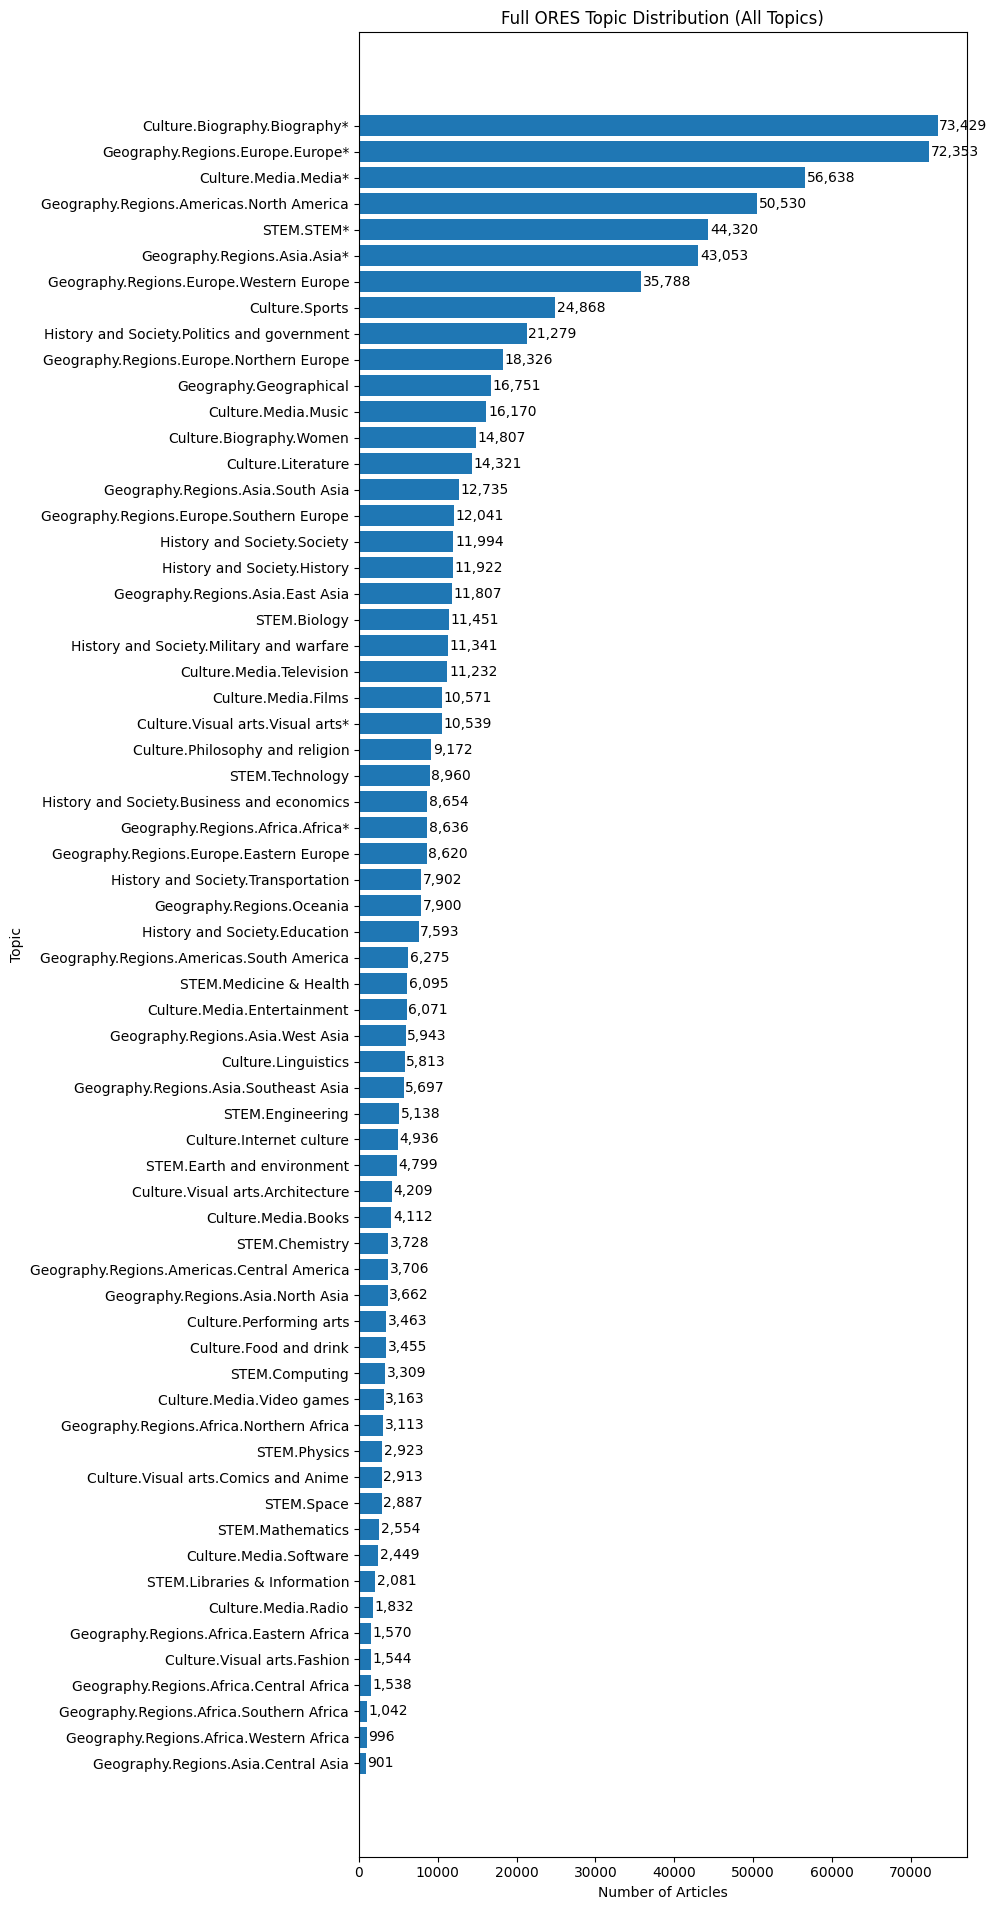
\includegraphics[width=0.6\textwidth]{img/FullORESTopicDist.png}
    \caption[Full distribution of ORES topics (all matched articles)]{\textbf{Full Distribution of ORES Topics (All Matched Articles).}
    The horizontal bar chart shows the count of matched Wikipedia articles assigned to each ORES fine-grained topic. The leading topics are Culture.Biography.Biography*, Geography.Regions.Europe.Europe*, Culture.Media.Media*, and Geography.Regions.Americas. Because an article can be assigned multiple topics, counts reflect topic assignments rather than unique articles. To manage this skew in subsequent analyses, we aggregate fine-grained topics into four main categories (Culture, Geography, STEM, History and Society) and apply weighted sampling when constructing evaluation subsets.}
    \label{fig:FullORESTopicDist}
\end{figure}

\begin{figure}[H]
    \centering
    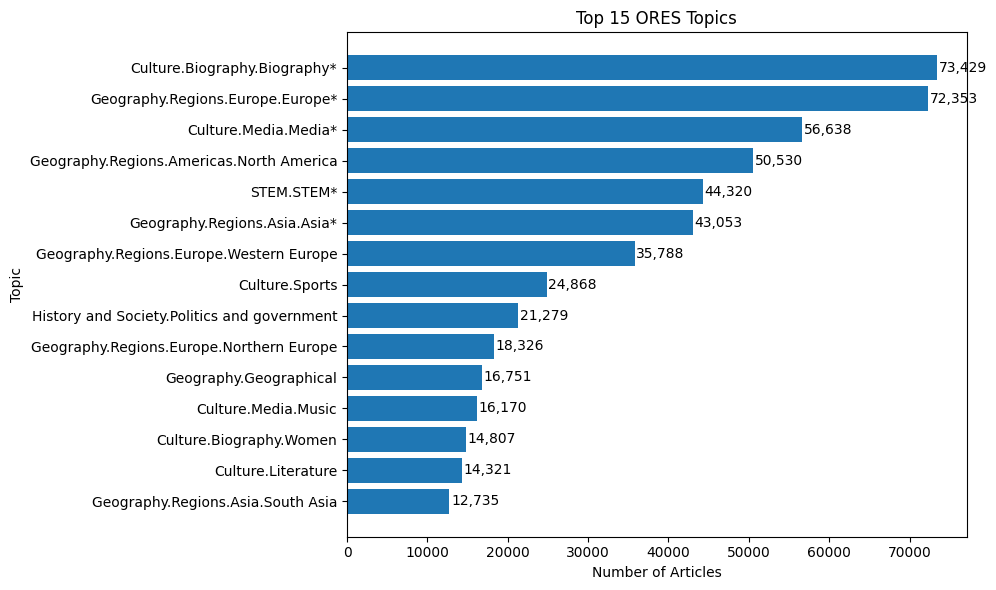
\includegraphics[width=1.0\textwidth]{img/FullORESTop15Dist.png}
    \caption[Top 15 ORES topics used for main‑topic assignment]{\textbf{Top 15 ORES Topics Used for Main‑Topic Assignment.}
    The chart shows the 15 most frequent fine-grained ORES topics in the matched dataset.
    In the midterm analysis we planned topic analysis at this fine-grained level. But, in the final analysis we aggregated topics into four main categories (Culture, Geography, STEM, History and Society).}
    \label{fig:FullORESTop15Dist}
\end{figure}

\begin{figure}[H]
    \centering
    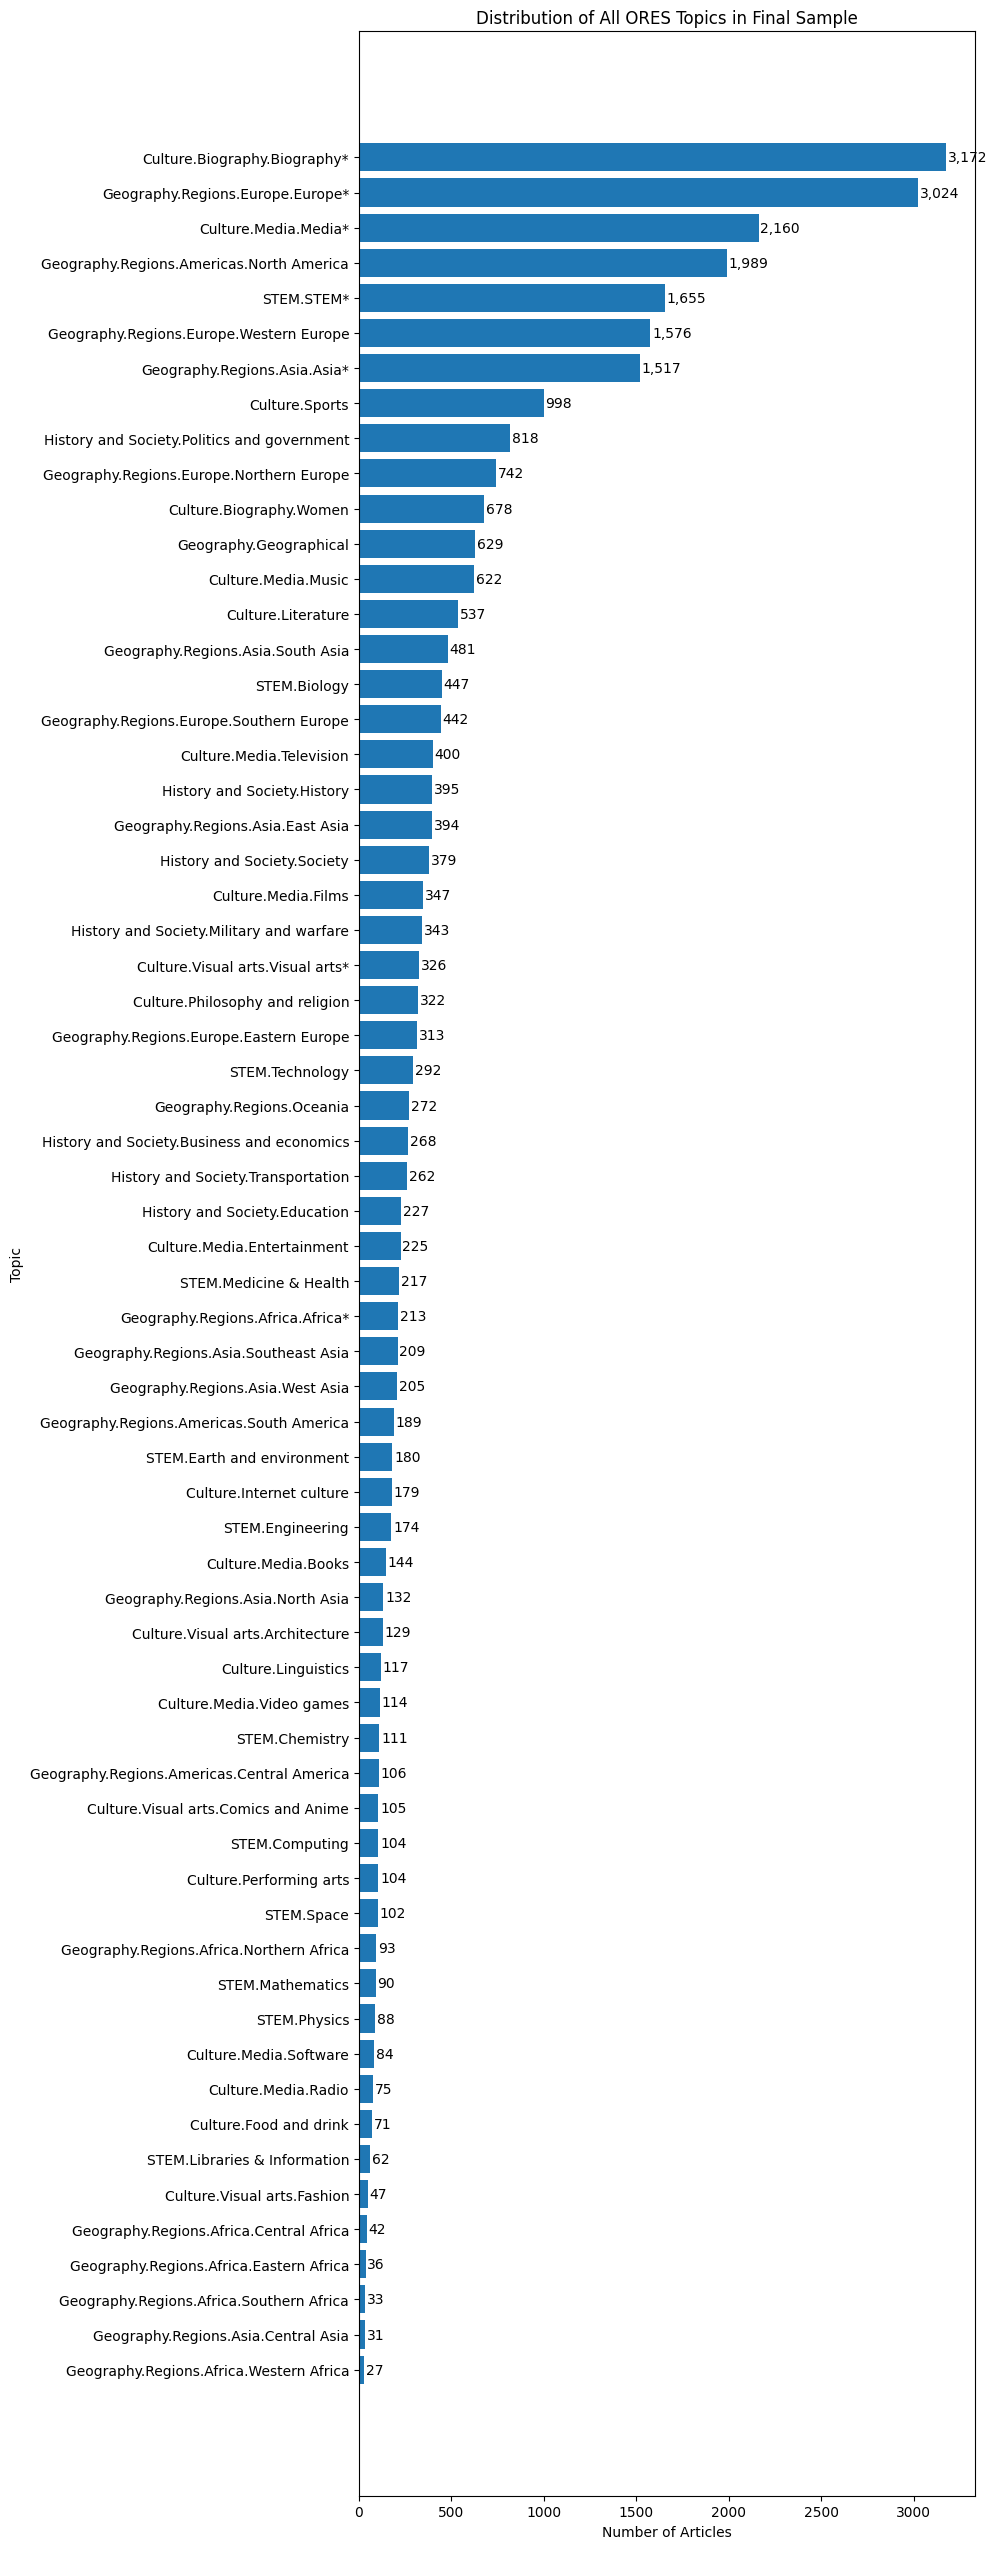
\includegraphics[width=0.5\textwidth]{img/10kORESTopicDist.png}
    \caption[Distribution of ORES topics in the final 10k sample]{\textbf{Distribution of ORES Topics in the Final 10k Sample.}
    The chart shows counts for all ORES fine-grained topics in the selected 10k article pairs before aggregating them into the four main categories (Culture, Geography, STEM, History and Society). The leading topics are Culture.Biography.Biography* and Geography.Regions.Europe.Europe* account for the largest shares, followed by Culture.Media.Media* and STEM.STEM*. And, the articles can have multiple topics, counts reflect topic assignments rather than unique articles.}
    \label{fig:10kORESTopicDist}
\end{figure}

\begin{figure}[H]
    \centering
    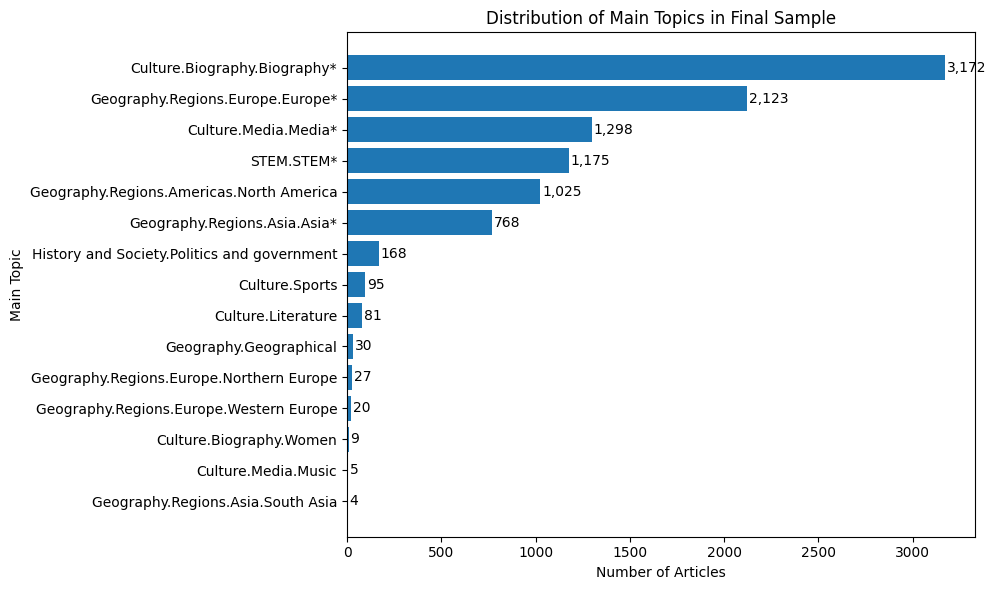
\includegraphics[width=1.0\textwidth]{img/10kORESTop15Dist.png}
    \caption[Distribution of main topics in the 10k sample]{\textbf{Distribution of Main Topics in the 10k Sample.}
    The chart shows the 15 most frequent fine-grained ORES topics among the 10k aligned article pairs. Because articles can have multiple topics, counts reflect topic assignments rather than unique articles. Results in the final analysis are reported at the four main-category level. This plot provides the fine-grained context of the final sample.}
    \label{fig:10kORESTop15Dist}
\end{figure}

\section{ORES Articletopic Taxonomy Overview}
\label{app:ORESHierarchy}
This figure shows the full taxonomy of the Articletopic model provided by the ORES system. It categorizes Wikipedia articles into a fine-grained hierarchy of topics across four main domains: \textbf{Culture}, \textbf{Geography}, \textbf{History and Society}, and \textbf{STEM}. This structure informs the mapping process described in \autoref{tab:TopicToCategoryMap}, where we combine fine-grained topics into four broader knowledge categories for analysis.

\begin{figure}[H]
    \centering
    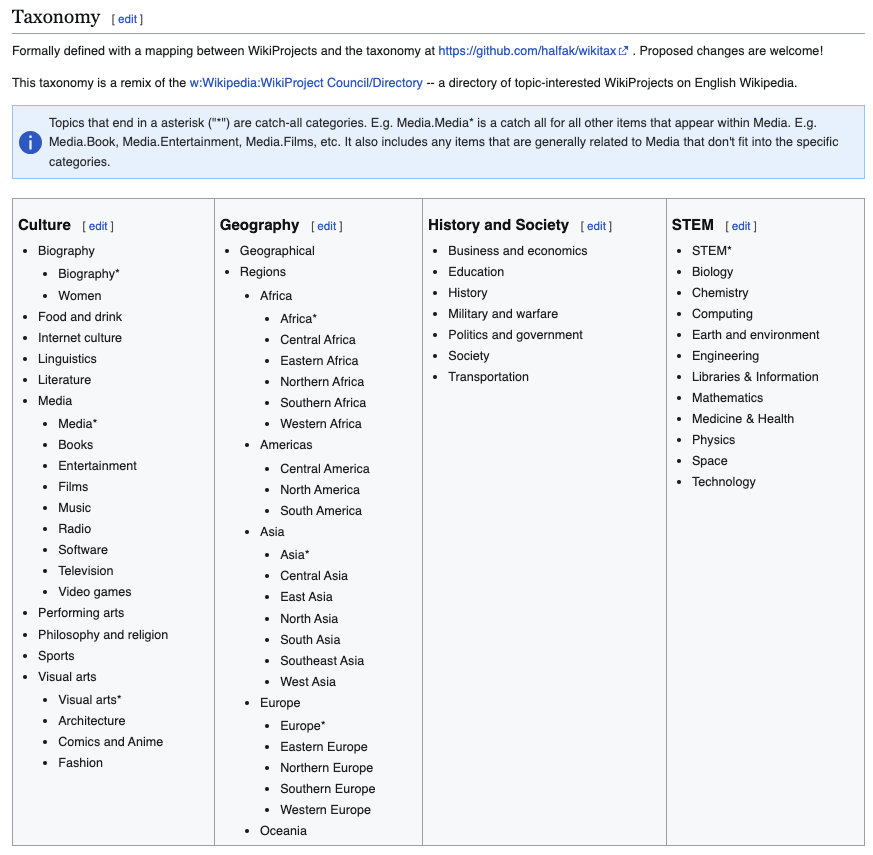
\includegraphics[width=1.0\textwidth]{img/ORES_Taxonomy_Tree.png}  
    \caption[Full taxonomy of the ORES Articletopic model]{\textbf{Full Taxonomy of the ORES Articletopic Model.} 
    The figure presents the complete hierarchical taxonomy used by the ORES Articletopic classifier to assign topical labels to Wikipedia articles. The taxonomy is divided into four main domains(Culture, Geography, History and Society, and STEM) each containing finer-grained subcategories. Examples include Biography, Media, and Sports under Culture, continental and regional divisions under Geography, Historical and Political under History and Society, and Biology, Computing, and Technology under STEM. 
    This taxonomy supports how we assign topics. It helps us group articles into broad categories.}
    \label{fig:ORESHierarchy}
\end{figure}


\section{Topic to Category Map}
\begin{table}[H]
\centering
\caption{Mapping of Top 15 ORES Topics to Four Main Categories}
\label{tab:TopicToCategoryMap}
\begin{tabular}{ll}
\toprule
\textbf{ORES Topic} & \textbf{Main Category} \\
\midrule
Culture.Biography.Biography* & Culture \\
Culture.Media.Media* & Culture \\
Culture.Sports & Culture \\
Culture.Literature & Culture \\
Culture.Media.Music & Culture \\
Culture.Biography.Women & Culture \\
Geography.Regions.Europe.Europe* & Geography \\
Geography.Regions.Americas.North America & Geography \\
Geography.Regions.Asia.Asia* & Geography \\
Geography.Geographical & Geography \\
Geography.Regions.Europe.Northern Europe & Geography \\
Geography.Regions.Europe.Western Europe & Geography \\
Geography.Regions.Asia.South Asia & Geography \\
STEM.STEM* & STEM \\
History and Society.Politics and government & History and Society \\
\bottomrule
\end{tabular}
\end{table}

\chapter{LLM Generation of Full Prompt Templates}
\label{appendix:prompts}

\enlargethispage{2\baselineskip}
For reproducibility, we include the full prompt used to query the LLMs in our experiments. 
The following template was programmatically instantiated with the English and Simple English Wikipedia paragraphs as inputs.


\begin{lstlisting}
You are a highly capable language model that specializes in semantic analysis and 
information retention between different versions of texts.

**Context**:
1. English Wikipedia:
{en_paragraph}

2. Simple English Wikipedia:
{simple_paragraph}

**Task**:
Analyze the two paragraphs and perform the following tasks:
1. Identify and list the key pieces of information that are retained in the Simple English version.
2. Identify and list the key pieces of information that are lost in the Simple English version.
3. Calculate the Semantic Retention Score as a percentage.

**Output Format (JSON)**:
{
    "Semantic Retention Score": "XX%",
    "Retained List": [
        "Fact 1",
        "Fact 2",
        ...
    ],
    "Lost List": [
        "Fact 1",
        "Fact 2",
        ...
    ]
}
\end{lstlisting}


\chapter{Qualitative Analysis: Case Study}
\section{Case Study Details}
\label{appendix:casestudy}
This appendix provides the full fact-level validation tables and metric summariesfor the case studies reported in Section~\ref{sec:case_study}.
For each article, we show (i) English Wikipedia vs.\ Simple English Wikipedia snippets, (ii) human vs.\ model fact-level comparison tables (LLaMA, Mistral, Gemma), and (iii) a metric summary(accuracy, F1).

\subsection{Case 1: Holliday Grainger}
\begin{figure}[H]
  \centering
  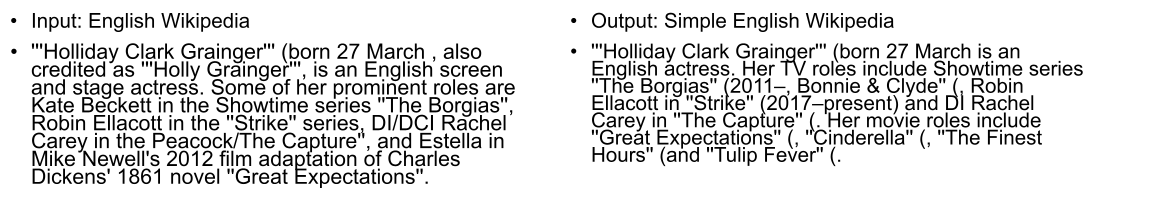
\includegraphics[width=\textwidth]{img/case_holliday_input_output.png}
  \caption[Case 1: Holliday Grainger – English vs. Simple English snippets]{\textbf{Case 1: Holliday Grainger – English vs. Simple English Snippets.} 
  The figure compares the first paragraph of the Holliday Grainger article in English Wikipedia (left) and Simple English Wikipedia (right). The English version provides detailed information such as alternative names, career highlights, and specific TV and film roles. In contrast, the Simple English version shortens sentences, removes alternative names, and simplifies descriptions of her acting roles. 
  This example illustrates how simplification reduces linguistic complexity and improves readability but also omits contextual and biographical details, demonstrating the trade-off between accessibility and information retention.}
  \label{fig:case_holliday}
\end{figure}

% ========= LLaMA vs Human =========
\begin{table}[H]
\centering
\resizebox{\textwidth}{!}{%
\begin{tabular}{p{7.2cm}cccc}
\toprule
\textbf{Facts by Human} & \textbf{Human Annotated List} & \textbf{LLaMA’s lists of} & \textbf{Validation Status} & \textbf{Validation} \\
\midrule
Holliday Clark Grainger was born on 27 March & Retained & Retained & True & TP \\
Holliday Clark Grainger is also credited as Holly Grainger & Lost & Not listed & Not listed & TN \\
Holliday Clark Grainger is an English screen actress & Retained & Retained & True & TP \\
Holliday Clark Grainger is an English stage actress & Lost & Not listed & Not listed & TN \\
Holliday Clark Grainger played Kate Beckett & Lost & Lost & True & TN \\
Kate Beckett appears in the Showtime series \textit{The Borgias} & Retained & Retained & True & TP \\
Holliday Clark Grainger played Robin Ellacott & Retained & Lost & False & FN \\
Robin Ellacott appears in the \textit{Strike} series & Retained & Retained & True & TP \\
Holliday Clark Grainger played DI/DCI Rachel Carey & Retained & Lost & False & FN \\
DI/DCI Rachel Carey appears in \textit{The Capture} & Retained & Lost & False & FN \\
\textit{The Capture} is streamed on Peacock & Lost & Not listed & Not listed & TN \\
Holliday Clark Grainger played Estella & Lost & Not listed & Not listed & TN \\
Estella appears in Mike Newell’s 2012 film adaptation & Lost & Not listed & Not listed & TN \\
Mike Newell’s film is an adaptation of \textit{Great Expectations} & Lost & Not listed & Not listed & TN \\
\textit{Great Expectations} is a novel by Charles Dickens & Lost & Not listed & Not listed & TN \\
\textit{Great Expectations} was published in 1861 & Lost & Lost & True & TN \\
\bottomrule
\end{tabular}%
}
\caption{\textit{Holliday Grainger} - Human vs.\ LLaMA fact comparison.}
\label{tab:holliday_llama}
\end{table}
% ========= Mistral vs Human =========
\begin{table}[H]
\centering
\resizebox{\textwidth}{!}{%
\begin{tabular}{p{7.2cm}cccc}
\toprule
\textbf{Facts by Human} & \textbf{Human Annotated List} & \textbf{Mistral’s lists of} & \textbf{Validation Status} & \textbf{Validation} \\
\midrule
Holliday Clark Grainger was born on 27 March & Retained & Not listed & Not listed & FN \\
Holliday Clark Grainger is also credited as Holly Grainger & Lost & Lost & True & TN \\
Holliday Clark Grainger is an English screen actress & Retained & Retained & True & TP \\
Holliday Clark Grainger is an English stage actress & Lost & Not listed & Not listed & TN \\
Holliday Clark Grainger played Kate Beckett & Lost & Not listed & Not listed & TN \\
Kate Beckett appears in the Showtime series \textit{The Borgias} & Retained & Retained & True & TP \\
Holliday Clark Grainger played Robin Ellacott & Retained & Retained & True & TP \\
Robin Ellacott appears in the \textit{Strike} series & Retained & Retained & True & TP \\
Holliday Clark Grainger played DI/DCI Rachel Carey & Retained & Retained & True & TP \\
DI/DCI Rachel Carey appears in \textit{The Capture} & Retained & Retained & True & TP \\
\textit{The Capture} is streamed on Peacock & Lost & Not listed & Not listed & TN \\
Holliday Clark Grainger played Estella & Lost & Not listed & Not listed & TN \\
Estella appears in Mike Newell’s 2012 film adaptation & Lost & Not listed & Not listed & TN \\
Mike Newell’s film is an adaptation of \textit{Great Expectations} & Lost & Not listed & Not listed & TN \\
\textit{Great Expectations} is a novel by Charles Dickens & Lost & Not listed & Not listed & TN \\
\textit{Great Expectations} was published in 1861 & Lost & Not listed & Not listed & TN \\
\bottomrule
\end{tabular}%
}
\caption{\textit{Holliday Grainger} - Human vs.\ Mistral fact comparison.}
\label{tab:holliday_mistral}
\end{table}
% ========= Gemma vs Human =========
\begin{table}[H]
\centering
\resizebox{\textwidth}{!}{%
\begin{tabular}{p{7.2cm}cccc}
\toprule
\textbf{Facts by Human} & \textbf{Human Annotated List} & \textbf{Gemma’s lists of} & \textbf{Validation Status} & \textbf{Validation} \\
\midrule
Holliday Clark Grainger was born on 27 March & Retained & Retained   & True       & TP \\
Holliday Clark Grainger is also credited as Holly Grainger & Lost & Lost & True       & TN \\
Holliday Clark Grainger is an English screen actress       & Retained & Retained & True & TP \\
Holliday Clark Grainger is an English stage actress        & Lost     & Not listed & Not listed & TN \\
Holliday Clark Grainger played Kate Beckett                & Lost     & Not listed & Not listed & TN \\
Kate Beckett appears in the Showtime series \textit{The Borgias} & Retained & Retained & True & TP \\
Holliday Clark Grainger played Robin Ellacott              & Retained & Not listed & Not listed & FN \\
Robin Ellacott appears in the \textit{Strike} series       & Retained & Retained & True & TP \\
Holliday Clark Grainger played DI/DCI Rachel Carey         & Retained & Not listed & Not listed & FN \\
DI/DCI Rachel Carey appears in \textit{The Capture}        & Retained & Retained & True & TP \\
\textit{The Capture} is streamed on Peacock                & Lost     & Not listed & Not listed & TN \\
Holliday Clark Grainger played Estella                     & Lost     & Not listed & Not listed & TN \\
Estella appears in Mike Newell’s 2012 film adaptation      & Lost     & Not listed & Not listed & TN \\
Mike Newell’s film is an adaptation of \textit{Great Expectations} & Lost & Not listed & Not listed & TN \\
\textit{Great Expectations} is a novel by Charles Dickens  & Lost     & Not listed & Not listed & TN \\
\textit{Great Expectations} was published in 1861          & Lost     & Not listed & Not listed & TN \\
\bottomrule
\end{tabular}%
}
\caption{\textit{Holliday Grainger} - Human vs.\ Gemma fact comparison.}
\label{tab:holliday_gemma}
\end{table}
% ========= Metric summary =========
\begin{table}[H]
\centering
\caption{\textit{Holliday Grainger} - metric summary (from fact-level validation).}
\label{tab:holliday_metrics}
\begin{tabular}{lcccc}
\toprule
\textbf{Model} & \textbf{Precision} & \textbf{Recall} & \textbf{Accuracy} & \textbf{F1} \\
\midrule
LLaMA   & 1.00 & 0.57 & 0.81 & 0.73 \\
Mistral & 1.00 & 0.86 & 0.94 & 0.92 \\
Gemma   & 1.00 & 0.72 & 0.86 & 0.84 \\
\bottomrule
\end{tabular}
\end{table}

\subsection{Case 2: Noguères}
\begin{figure}[H]
  \centering
  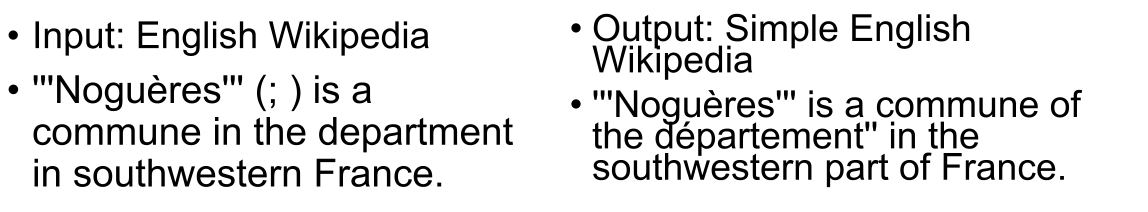
\includegraphics[width=\textwidth]{img/case_nogueres_input_output.png}
  \caption[Case 2: Noguères – English vs. Simple English snippets]{\textbf{Case 2: Noguères – English vs. Simple English Snippets.} 
  The figure compares the English Wikipedia and Simple English Wikipedia versions of the article on the commune Noguères. The English snippet briefly states that Noguères is a commune in the department in southwestern France. The Simple English version makes a slight structural change, rephrasing it as “a commune of the département in the southwestern part of France,” while maintaining the core meaning. 
  This example shows how simplification does not always involve major deletions but may instead manifest in minor lexical or structural adjustments. Such cases highlight the variability of simplification strategies and their differing impact on information retention.}
  \label{fig:case_nogueres}
\end{figure}

% ========= LLaMA vs Human =========
\begin{table}[H]
\centering
\resizebox{0.8\textwidth}{!}{%
\begin{tabular}{p{7.2cm}cccc}
\toprule
\textbf{Facts by Human} & \textbf{Human Annotated List} & \textbf{LLaMA’s lists of} & \textbf{Validation Status} & \textbf{Validation} \\
\midrule
Noguères is a commune & Retained & Retained & True & TP \\
Noguères is located in a department in southwestern France & Retained & Retained & True & TP \\
\bottomrule
\end{tabular}%
}
\caption{\textit{Noguères} - Human vs.\ LLaMA fact comparison.}
\label{tab:nogueres_llama}
\end{table}
% ========= Mistral vs Human =========
\begin{table}[H]
\centering
\resizebox{0.8\textwidth}{!}{%
\begin{tabular}{p{7.2cm}cccc}
\toprule
\textbf{Facts by Human} & \textbf{Human Annotated List} & \textbf{Mistral’s lists of} & \textbf{Validation Status} & \textbf{Validation} \\
\midrule
Noguères is a commune & Retained & Retained & True & TP \\
Noguères is located in a department in southwestern France & Retained & Retained & True & TP \\
\bottomrule
\end{tabular}%
}
\caption{\textit{Noguères} - Human vs.\ Mistral fact comparison.}
\label{tab:nogueres_mistral}
\end{table}
% ========= Gemma vs Human =========
\begin{table}[H]
\centering
\resizebox{0.8\textwidth}{!}{%
\begin{tabular}{p{7.2cm}cccc}
\toprule
\textbf{Facts by Human} & \textbf{Human Annotated List} & \textbf{Gemma’s lists of} & \textbf{Validation Status} & \textbf{Validation} \\
\midrule
Noguères is a commune & Retained & Retained & True & TP \\
Noguères is located in a department in southwestern France & Retained & Retained & True & TP \\
\bottomrule
\end{tabular}%
}
\caption{\textit{Noguères} - Human vs.\ Gemma fact comparison.}
\label{tab:nogueres_gemma}
\end{table}
% ========= Metric summary =========
\begin{table}[H]
\centering
\caption{\textit{Noguères} - metric summary (from fact-level validation).}
\label{tab:nogueres_metrics}
\begin{tabular}{lcccc}
\toprule
\textbf{Model} & \textbf{Precision} & \textbf{Recall} & \textbf{Accuracy} & \textbf{F1} \\
\midrule
LLaMA   & 1.00 & 1.00 & 1.00 & 1.00 \\
Mistral & 1.00 & 1.00 & 1.00 & 1.00 \\
Gemma   & 1.00 & 1.00 & 1.00 & 1.00 \\
\bottomrule
\end{tabular}
\end{table}

\subsection{Case 3: The Lonely White Sail}
\begin{figure}[H]
  \centering
  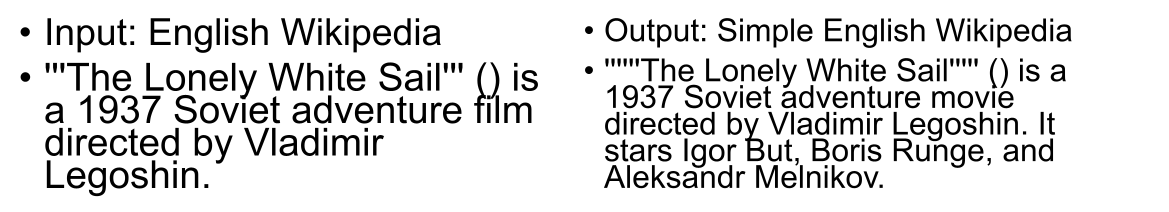
\includegraphics[width=\textwidth]{img/case_lonely_input_output.png} 
  \caption[Case 3: The Lonely White Sail – English vs. Simple English snippets]{\textbf{Case 3: The Lonely White Sail – English vs. Simple English Snippets.} 
  The figure compares the English and Simple English Wikipedia entries for the 1937 Soviet film The Lonely White Sail. The English snippet states only the film’s title, release year, genre, and director. The Simple English version conveys the same core information but adds extra details, including the main actors Igor But, Boris Runge, and Aleksandr Melnikov, while also using the simpler word “movie” instead of “film.” 
  This example illustrates how simplification can lead to the omission of critical details, particularly in topics involving sensitive political or ethical perspective.}
  \label{fig:case_lonely}
\end{figure}

% ========= LLaMA vs Human =========
\begin{table}[H]
\centering
\resizebox{0.9\textwidth}{!}{%
\begin{tabular}{p{8.5cm}cccc}
\toprule
\textbf{Facts by Human} & \textbf{Human Annotated List} & \textbf{LLaMA’s lists of} & \textbf{Validation Status} & \textbf{Validation} \\
\midrule
The Lonely White Sail is a 1937 Soviet adventure film & Retained & Retained & True & TP \\
The Lonely White Sail was directed by Vladimir Legoshin & Retained & Lost & False & FN \\
\bottomrule
\end{tabular}%
}
\caption{\textit{The Lonely White Sail} - Human vs.\ LLaMA fact comparison.}
\label{tab:lonely_llama}
\end{table}

% ========= Mistral vs Human =========
\begin{table}[H]
\centering
\resizebox{0.9\textwidth}{!}{%
\begin{tabular}{p{8.5cm}cccc}
\toprule
\textbf{Facts by Human} & \textbf{Human Annotated List} & \textbf{Mistral’s lists of} & \textbf{Validation Status} & \textbf{Validation} \\
\midrule
The Lonely White Sail is a 1937 Soviet adventure film & Retained & Not listed & Not listed & FN \\
The Lonely White Sail was directed by Vladimir Legoshin & Retained & Not listed & Not listed & FN \\
\bottomrule
\end{tabular}%
}
\caption{\textit{The Lonely White Sail} - Human vs.\ Mistral fact comparison.}
\label{tab:lonely_mistral}
\end{table}

% ========= Gemma vs Human =========
\begin{table}[H]
\centering
\resizebox{0.9\textwidth}{!}{%
\begin{tabular}{p{8.5cm}cccc}
\toprule
\textbf{Facts by Human} & \textbf{Human Annotated List} & \textbf{Gemma’s lists of} & \textbf{Validation Status} & \textbf{Validation} \\
\midrule
The Lonely White Sail is a 1937 Soviet adventure film & Retained & Not listed & Not listed & FN \\
The Lonely White Sail was directed by Vladimir Legoshin & Retained & Retained & True & TP \\
\bottomrule
\end{tabular}%
}
\caption{\textit{The Lonely White Sail} - Human vs.\ Gemma fact comparison.}
\label{tab:lonely_gemma}
\end{table}

% ========= Metric summary =========
\begin{table}[H]
\centering
\caption{\textit{The Lonely White Sail} - metric summary (from fact-level validation).}
\label{tab:lonely_metrics}
\begin{tabular}{lcccc}
\toprule
\textbf{Model} & \textbf{Precision} & \textbf{Recall} & \textbf{Accuracy} & \textbf{F1} \\
\midrule
LLaMA   & 1.00 & 0.50 & 0.50 & 0.67 \\
Mistral & 0.00 & 0.00 & 0.00 & 0.00 \\
Gemma   & 1.00 & 0.50 & 0.50 & 0.67 \\
\bottomrule
\end{tabular}
\end{table}

\subsection{Case 4: Black Sites}
\begin{figure}[H]
  \centering
  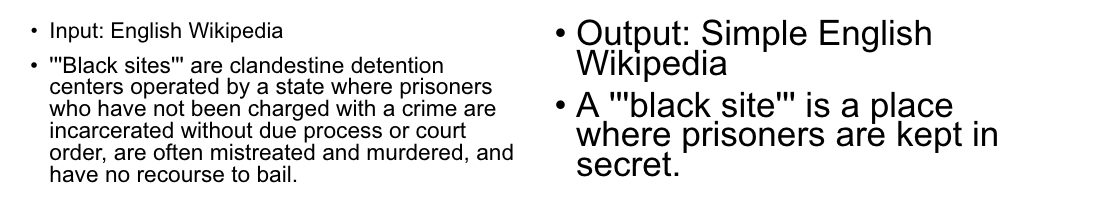
\includegraphics[width=\textwidth]{img/case_blacksite_input_output.png}
  \caption[Case 4: Black Sites – English vs. Simple English snippets]{\textbf{Case 4: Black Sites – English vs. Simple English Snippets.} 
  The English Wikipedia snippet describes black sites as clandestine detention centers run by states, highlighting issues such as lack of due process, mistreatment, and denial of bail. The Simple English version simplifies the phrasing while retaining some sensitive details, though not all. This example shows how simplification in politically or ethically charged topics may alter the balance between institutional description and human rights concerns.}
  \label{fig:case_blacksite}
\end{figure}

% ========= LLaMA vs Human =========
\begin{table}[H]
\centering
\resizebox{\textwidth}{!}{%
\begin{tabular}{p{7.5cm}cccc}
\toprule
\textbf{Facts by Human} & \textbf{Human Annotated List} & \textbf{LLaMA’s lists of} & \textbf{Validation Status} & \textbf{Validation} \\
\midrule
Black sites are clandestine detention centers operated by a state. & Retained & Retained & True & TP \\
Prisoners in black sites are often incarcerated without being charged with a crime. & Lost & Not listed & Not listed & TN \\
Prisoners in black sites are held without due process or court order. & Lost & Retained & False & FP \\
Prisoners in black sites are often mistreated. & Lost & Lost & True & TN \\
Prisoners in black sites are sometimes murdered. & Lost & Lost & True & TN \\
Prisoners in black sites have no recourse to bail. & Lost & Retained & False & FP \\
\bottomrule
\end{tabular}%
}
\caption{\textit{Black Sites} - Human vs.\ LLaMA fact comparison.}
\label{tab:blacksite_llama}
\end{table}

% ========= Mistral vs Human =========
\begin{table}[H]
\centering
\resizebox{\textwidth}{!}{%
\begin{tabular}{p{7.5cm}cccc}
\toprule
\textbf{Facts by Human} & \textbf{Human Annotated List} & \textbf{Mistral’s lists of} & \textbf{Validation Status} & \textbf{Validation} \\
\midrule
Black sites are clandestine detention centers operated by a state. & Retained & Lost & False & FN \\
Prisoners in black sites are often incarcerated without being charged with a crime. & Lost & Lost & True & TN \\
Prisoners in black sites are held without due process or court order. & Lost & Lost & True & TN \\
Prisoners in black sites are often mistreated. & Lost & Lost & True & TN \\
Prisoners in black sites are sometimes murdered. & Lost & Lost & True & TN \\
Prisoners in black sites have no recourse to bail. & Lost & Lost & True & TN \\
\bottomrule
\end{tabular}%
}
\caption{\textit{Black Sites} - Human vs.\ Mistral fact comparison.}
\label{tab:blacksite_mistral}
\end{table}

% ========= Gemma vs Human =========
\begin{table}[H]
\centering
\resizebox{\textwidth}{!}{%
\begin{tabular}{p{7.5cm}cccc}
\toprule
\textbf{Facts by Human} & \textbf{Human Annotated List} & \textbf{Gemma’s lists of} & \textbf{Validation Status} & \textbf{Validation} \\
\midrule
Black sites are clandestine detention centers operated by a state. & Retained & Retained & True & TP \\
Prisoners in black sites are often incarcerated without being charged with a crime. & Lost & Not listed & Not listed & TN \\
Prisoners in black sites are held without due process or court order. & Lost & Not listed & Not listed & TN \\
Prisoners in black sites are often mistreated. & Lost & Lost & True & TN \\
Prisoners in black sites are sometimes murdered. & Lost & Lost & True & TN \\
Prisoners in black sites have no recourse to bail. & Lost & Lost & True & TN \\
\bottomrule
\end{tabular}%
}
\caption{\textit{Black Sites} - Human vs.\ Gemma fact comparison.}
\label{tab:blacksite_gemma}
\end{table}

% ========= Metric summary =========
\begin{table}[H]
\centering
\caption{\textit{Black Sites} - metric summary (from fact-level validation).}
\label{tab:blacksite_metrics}
\begin{tabular}{lcccc}
\toprule
\textbf{Model} & \textbf{Precision} & \textbf{Recall} & \textbf{Accuracy} & \textbf{F1} \\
\midrule
LLaMA   & 0.33 & 1.00 & 0.67 & 0.50 \\
Mistral & 0.00 & 0.00 & 0.83 & 0.00 \\
Gemma   & 1.00 & 1.00 & 1.00 & 1.00 \\
\bottomrule
\end{tabular}
\end{table}




\subsection{Case 5: Bureau of Indian Affairs}
\begin{figure}[H]
  \centering
  
\includegraphics[width=\textwidth]{img/case_Bureau_input_output.png}
  \caption[Case 4: Bureau of Indian Affairs – English vs. Simple English snippets]{\textbf{Case 4: Bureau of Indian Affairs – English vs. Simple English Snippets.} 
  The figure compares the English and Simple English Wikipedia entries for the Bureau of Indian Affairs (BIA), a U.S. federal agency. The English snippet emphasizes institutional details such as legal responsibilities, governance structure, and population coverage. The Simple English version, however, focuses on historical background (founded in 1824), functional responsibilities (land, resources, law enforcement), and education services (via the Bureau of Indian Education). 
  This example shows how simplification can shift emphasis by leaving out bureaucratic details while highlighting historical and practical aspects.}
  \label{fig:case_Bureau}
\end{figure}

% ========= LLaMA vs Human =========
\begin{table}[H]
\centering
\resizebox{\textwidth}{!}{%
\begin{tabular}{p{7.5cm}cccc}
\toprule
\textbf{Facts by Human} & \textbf{Human Annotated List} & \textbf{LLaMA’s lists of} & \textbf{Validation Status} & \textbf{Validation} \\
\midrule
The Bureau of Indian Affairs is also known as Indian Affairs & Lost & Not listed & Not listed & TN \\
The Bureau of Indian Affairs is abbreviated as BIA & Retained & Not listed & Not listed & FN \\
Indian Affairs is abbreviated as IA & Lost & Not listed & Not listed & TN \\
The Bureau of Indian Affairs is a United States federal agency & Lost & Lost & True & TN \\
The Bureau of Indian Affairs is within the Department of the Interior & Lost & Lost & True & TN \\
The Bureau of Indian Affairs is responsible for implementing federal laws related to Native Americans & Lost & Not listed & Not listed & TN \\
The Bureau of Indian Affairs is responsible for implementing federal policies related to Native Americans & Lost & Not listed & Not listed & TN \\
The Bureau of Indian Affairs is responsible for reservations held in trust by the U.S. government & Lost & Not listed & Not listed & TN \\
The U.S. federal government holds reservations in trust for indigenous tribes & Lost & Not listed & Not listed & TN \\
The Bureau of Indian Affairs renders services to roughly 2 million indigenous Americans & Lost & Lost & True & TN \\
The Bureau of Indian Affairs serves 574 federally recognized tribes & Lost & Lost & True & TN \\
The Bureau of Indian Affairs is governed by a director & Lost & Lost & True & TN \\
The Bureau of Indian Affairs is overseen by the Assistant Secretary for Indian Affairs & Lost & Lost & True & TN \\
The Assistant Secretary for Indian Affairs answers to the Secretary of the Interior & Lost & Lost & True & TN \\
\bottomrule
\end{tabular}%
}
\caption{\textit{Bureau of Indian Affairs} - Human vs.\ LLaMA fact comparison.}
\label{tab:bia_llama}
\end{table}

% ========= Mistral vs Human =========
\begin{table}[H]
\centering
\resizebox{\textwidth}{!}{%
\begin{tabular}{p{7.5cm}cccc}
\toprule
\textbf{Facts by Human} & \textbf{Human Annotated List} & \textbf{Mistral’s lists of} & \textbf{Validation Status} & \textbf{Validation} \\
\midrule
The Bureau of Indian Affairs is also known as Indian Affairs & Lost & Retained & False & FP \\
The Bureau of Indian Affairs is abbreviated as BIA & Retained & Retained & True & TP \\
Indian Affairs is abbreviated as IA & Lost & Retained & False & FP \\
The Bureau of Indian Affairs is a United States federal agency & Lost & Retained & False & FP \\
The Bureau of Indian Affairs is within the Department of the Interior & Lost & Retained & False & FP \\
The Bureau of Indian Affairs is responsible for implementing federal laws related to Native Americans & Lost & Lost & True & TN \\
The Bureau of Indian Affairs is responsible for implementing federal policies related to Native Americans & Lost & Lost & True & TN \\
The Bureau of Indian Affairs is responsible for reservations held in trust by the U.S. government & Lost & Lost & True & TN \\
The U.S. federal government holds reservations in trust for indigenous tribes & Lost & Lost & True & TN \\
The Bureau of Indian Affairs renders services to roughly 2 million indigenous Americans & Lost & Retained & False & FP \\
The Bureau of Indian Affairs serves 574 federally recognized tribes & Lost & Retained & False & FP \\
The Bureau of Indian Affairs is governed by a director & Lost & Lost & True & TN \\
The Bureau of Indian Affairs is overseen by the Assistant Secretary for Indian Affairs & Lost & Lost & True & TN \\
The Assistant Secretary for Indian Affairs answers to the Secretary of the Interior & Lost & Lost & True & TN \\
\bottomrule
\end{tabular}%
}
\caption{\textit{Bureau of Indian Affairs} - Human vs.\ Mistral fact comparison.}
\label{tab:bia_mistral}
\end{table}

% ========= Gemma vs Human =========
\begin{table}[H]
\centering
\resizebox{\textwidth}{!}{%
\begin{tabular}{p{7.5cm}cccc}
\toprule
\textbf{Facts by Human} & \textbf{Human Annotated List} & \textbf{Gemma’s lists of} & \textbf{Validation Status} & \textbf{Validation} \\
\midrule
The Bureau of Indian Affairs is also known as Indian Affairs & Lost & Not listed & Not listed & TN \\
The Bureau of Indian Affairs is abbreviated as BIA & Retained & Not listed & Not listed & FN \\
Indian Affairs is abbreviated as IA & Lost & Not listed & Not listed & TN \\
The Bureau of Indian Affairs is a United States federal agency & Lost & Not listed & Not listed & TN \\
The Bureau of Indian Affairs is within the Department of the Interior & Lost & Not listed & Not listed & TN \\
The Bureau of Indian Affairs is responsible for implementing federal laws related to Native Americans & Lost & Lost & True & TN \\
The Bureau of Indian Affairs is responsible for implementing federal policies related to Native Americans & Lost & Lost & True & TN \\
The Bureau of Indian Affairs is responsible for reservations held in trust by the U.S. government & Lost & Lost & True & TN \\
The U.S. federal government holds reservations in trust for indigenous tribes & Lost & Lost & True & TN \\
The Bureau of Indian Affairs renders services to roughly 2 million indigenous Americans & Lost & Lost & True & TN \\
The Bureau of Indian Affairs serves 574 federally recognized tribes & Lost & Lost & True & TN \\
The Bureau of Indian Affairs is governed by a director & Lost & Lost & True & TN \\
The Bureau of Indian Affairs is overseen by the Assistant Secretary for Indian Affairs & Lost & Lost & True & TN \\
The Assistant Secretary for Indian Affairs answers to the Secretary of the Interior & Lost & Not listed & Not listed & TN \\
\bottomrule
\end{tabular}%
}
\caption{\textit{Bureau of Indian Affairs} - Human vs.\ Gemma fact comparison.}
\label{tab:bia_gemma}
\end{table}

% ========= Metric summary =========
\begin{table}[H]
\centering
\caption{\textit{Bureau of Indian Affairs} - metric summary (from fact-level validation).}
\label{tab:bia_metrics}
\begin{tabular}{lcccc}
\toprule
\textbf{Model} & \textbf{Precision} & \textbf{Recall} & \textbf{Accuracy} & \textbf{F1} \\
\midrule
LLaMA   & 0.00 & 0.00 & 0.93 & 0.00 \\
Mistral & 0.14 & 1.00 & 0.57 & 0.26 \\
Gemma   & 0.00 & 0.00 & 1.00 & 0.00 \\
\bottomrule
\end{tabular}
\end{table}

\subsection{Case 6: Enhanced Geothermal Systems (EGS)}
\begin{figure}[H]
  \centering
  \includegraphics[width=\textwidth]{img/case_egs_input_output.png} 
  \caption[Case 5: Enhanced Geothermal Systems – English vs. Simple English snippets]{\textbf{Case 5: Enhanced Geothermal Systems – English vs. Simple English Snippets.} 
  The English Wikipedia snippet introduces the concept of an Enhanced Geothermal System (EGS), highlighting its use of convective hydrothermal resources. The Simple English version simplifies the terminology but also includes explanatory context about simulation methods such as hydraulic stimulation. This illustrates how simplification may adjust technical vocabulary and reframe information with practical examples.}
  \label{fig:case_egs}
\end{figure}
% ========= LLaMA vs Human =========
\begin{table}[H]
\centering
\resizebox{0.95\textwidth}{!}{%
\begin{tabular}{p{8.5cm}cccc}
\toprule
\textbf{Facts by Human} & \textbf{Human Annotated List} & \textbf{LLaMA’s lists of} & \textbf{Validation Status} & \textbf{Validation} \\
\midrule
An enhanced geothermal system (EGS) generates convective hydrothermal resources. & Retained & Retained & True & TP \\
Traditional geothermal power systems operate only where naturally occurring heat, water, and rock permeability are sufficient for energy extraction. & Lost & Lost & True & TN \\
Most geothermal energy within reach of conventional techniques is in dry and impermeable rock. & Lost & Lost & True & TN \\
EGS technologies expand geothermal resource availability. & Lost & Lost & True & TN \\
EGS achieves this through simulation methods. & Lost & Not listed & True & TN \\
One such simulation method is hydraulic stimulation. & Lost & Lost & True & TN \\
\bottomrule
\end{tabular}%
}
\caption{\textit{Enhanced Geothermal Systems} - Human vs.\ LLaMA fact comparison.}
\label{tab:egs_llama}
\end{table}

% ========= Mistral vs Human =========
\begin{table}[H]
\centering
\resizebox{0.95\textwidth}{!}{%
\begin{tabular}{p{8.5cm}cccc}
\toprule
\textbf{Facts by Human} & \textbf{Human Annotated List} & \textbf{Mistral’s lists of} & \textbf{Validation Status} & \textbf{Validation} \\
\midrule
An enhanced geothermal system (EGS) generates convective hydrothermal resources. & Retained & Lost & True & TN \\
Traditional geothermal power systems operate only where naturally occurring heat, water, and rock permeability are sufficient for energy extraction. & Lost & Lost & True & TN \\
Most geothermal energy within reach of conventional techniques is in dry and impermeable rock. & Lost & Lost & True & TN \\
EGS technologies expand geothermal resource availability. & Lost & Lost & True & TN \\
EGS achieves this through simulation methods. & Lost & Lost & True & TN \\
One such simulation method is hydraulic stimulation. & Lost & Lost & True & TN \\
\bottomrule
\end{tabular}%
}
\caption{\textit{Enhanced Geothermal Systems} - Human vs.\ Mistral fact comparison.}
\label{tab:egs_mistral}
\end{table}

% ========= Gemma vs Human =========
\begin{table}[H]
\centering
\resizebox{0.95\textwidth}{!}{%
\begin{tabular}{p{8.5cm}cccc}
\toprule
\textbf{Facts by Human} & \textbf{Human Annotated List} & \textbf{Gemma’s lists of} & \textbf{Validation Status} & \textbf{Validation} \\
\midrule
An enhanced geothermal system (EGS) generates convective hydrothermal resources. & Retained & Retained & True & TP \\
Traditional geothermal power systems operate only where naturally occurring heat, water, and rock permeability are sufficient for energy extraction. & Lost & Lost & True & TN \\
Most geothermal energy within reach of conventional techniques is in dry and impermeable rock. & Lost & Lost & True & TN \\
EGS technologies expand geothermal resource availability. & Lost & Retained & False & FN \\
EGS achieves this through simulation methods. & Lost & Lost & True & TN \\
One such simulation method is hydraulic stimulation. & Lost & Lost & True & TN \\
\bottomrule
\end{tabular}%
}
\caption{\textit{Enhanced Geothermal Systems} - Human vs.\ Gemma fact comparison.}
\label{tab:egs_gemma}
\end{table}

% ========= Metric summary =========
\begin{table}[H]
\centering
\caption{\textit{Enhanced Geothermal Systems} - metric summary (from fact-level validation).}
\label{tab:egs_metrics}
\begin{tabular}{lcccc}
\toprule
\textbf{Model} & \textbf{Precision} & \textbf{Recall} & \textbf{Accuracy} & \textbf{F1} \\
\midrule
LLaMA   & 1.00 & 1.00 & 1.00 & 1.00 \\
Mistral & 0.00 & 0.00 & 1.00 & 0.00 \\
Gemma   & 1.00 & 1.00 & 0.83 & 1.00 \\
\bottomrule
\end{tabular}
\end{table}

%%%%%%%%%%%%%%%%%%%%% Bibliography %%%%%%%%%%%%%%%%%%%%%% 
\addcontentsline{toc}{chapter}{Bibliography}
\printbibliography
\end{document}  